%2multibyte Version: 5.50.0.2953 CodePage: 1252
%% Macros for Scientific Word 2.5 documents saved with the LaTeX filter.
%Copyright (C) 1994-96 TCI Software Research, Inc.
\typeout{TCILATEX Macros for Scientific Word 2.5 <04 SEP 96>.}

\typeout{NOTICE:  This macro file is NOT proprietary and may be 
freely copied and distributed.}


\makeatletter
%%
%% Changes
%% ** to \def\readFRAMEparams
%%    replaces h by H, if the float package is loaded
%%
\@ifundefined{@HHfloat}{\relax}{\typeout{** TCILaTeX detected 'float'-package:}	}	
%%see changes
%
%%%%%%%%%%%%%%%%%%%%%%
% macros for time
\newcount\@hour\newcount\@minute\chardef\@x10\chardef\@xv60
\def\tcitime{
\def\@time{%
  \@minute\time\@hour\@minute\divide\@hour\@xv
  \ifnum\@hour<\@x 0\fi\the\@hour:%
  \multiply\@hour\@xv\advance\@minute-\@hour
  \ifnum\@minute<\@x 0\fi\the\@minute
  }}%

%%%%%%%%%%%%%%%%%%%%%%
% macro for hyperref
\@ifundefined{hyperref}{\def\hyperref#1#2#3#4{#2\ref{#4}#3}}{}

% macro for external program call
\@ifundefined{qExtProgCall}{\def\qExtProgCall#1#2#3#4#5#6{\relax}}{}
%%%%%%%%%%%%%%%%%%%%%%
%
% macros for graphics
%
\def\FILENAME#1{#1}%
%
\def\QCTOpt[#1]#2{%
  \def\QCTOptB{#1}
  \def\QCTOptA{#2}
}
\def\QCTNOpt#1{%
  \def\QCTOptA{#1}
  \let\QCTOptB\empty
}
\def\Qct{%
  \@ifnextchar[{%
    \QCTOpt}{\QCTNOpt}
}
\def\QCBOpt[#1]#2{%
  \def\QCBOptB{#1}
  \def\QCBOptA{#2}
}
\def\QCBNOpt#1{%
  \def\QCBOptA{#1}
  \let\QCBOptB\empty
}
\def\Qcb{%
  \@ifnextchar[{%
    \QCBOpt}{\QCBNOpt}
}
\def\PrepCapArgs{%
  \ifx\QCBOptA\empty
    \ifx\QCTOptA\empty
      {}%
    \else
      \ifx\QCTOptB\empty
        {\QCTOptA}%
      \else
        [\QCTOptB]{\QCTOptA}%
      \fi
    \fi
  \else
    \ifx\QCBOptA\empty
      {}%
    \else
      \ifx\QCBOptB\empty
        {\QCBOptA}%
      \else
        [\QCBOptB]{\QCBOptA}%
      \fi
    \fi
  \fi
}
\newcount\GRAPHICSTYPE
%\GRAPHICSTYPE 0 is for TurboTeX
%\GRAPHICSTYPE 1 is for DVIWindo (PostScript)
%%%(removed)%\GRAPHICSTYPE 2 is for psfig (PostScript)
\GRAPHICSTYPE=\z@
\def\GRAPHICSPS#1{%
 \ifcase\GRAPHICSTYPE%\GRAPHICSTYPE=0
   \special{ps: #1}%
 \or%\GRAPHICSTYPE=1
   \special{language "PS", include "#1"}%
%%%\or%\GRAPHICSTYPE=2
%%%  #1%
 \fi
}%
%
\def\GRAPHICSHP#1{\special{include #1}}%
%
% \graffile{ body }                                  %#1
%          { contentswidth (scalar)  }               %#2
%          { contentsheight (scalar) }               %#3
%          { vertical shift when in-line (scalar) }  %#4
\def\graffile#1#2#3#4{%
%%% \ifnum\GRAPHICSTYPE=\tw@
%%%  %Following if using psfig
%%%  \@ifundefined{psfig}{\input psfig.tex}{}%
%%%  \psfig{file=#1, height=#3, width=#2}%
%%% \else
  %Following for all others
  % JCS - added BOXTHEFRAME, see below
    \leavevmode
    \raise -#4 \BOXTHEFRAME{%
        \hbox to #2{\raise #3\hbox to #2{\null #1\hfil}}}%
}%
%
% A box for drafts
\def\draftbox#1#2#3#4{%
 \leavevmode\raise -#4 \hbox{%
  \frame{\rlap{\protect\tiny #1}\hbox to #2%
   {\vrule height#3 width\z@ depth\z@\hfil}%
  }%
 }%
}%
%
\newcount\draft
\draft=\z@
\let\nographics=\draft
\newif\ifwasdraft
\wasdraftfalse

%  \GRAPHIC{ body }                                  %#1
%          { draft name }                            %#2
%          { contentswidth (scalar)  }               %#3
%          { contentsheight (scalar) }               %#4
%          { vertical shift when in-line (scalar) }  %#5
\def\GRAPHIC#1#2#3#4#5{%
 \ifnum\draft=\@ne\draftbox{#2}{#3}{#4}{#5}%
  \else\graffile{#1}{#3}{#4}{#5}%
  \fi
 }%
%
\def\addtoLaTeXparams#1{%
    \edef\LaTeXparams{\LaTeXparams #1}}%
%
% JCS -  added a switch BoxFrame that can 
% be set by including X in the frame params.
% If set a box is drawn around the frame.

\newif\ifBoxFrame \BoxFramefalse
\newif\ifOverFrame \OverFramefalse
\newif\ifUnderFrame \UnderFramefalse

\def\BOXTHEFRAME#1{%
   \hbox{%
      \ifBoxFrame
         \frame{#1}%
      \else
         {#1}%
      \fi
   }%
}


\def\doFRAMEparams#1{\BoxFramefalse\OverFramefalse\UnderFramefalse\readFRAMEparams#1\end}%
\def\readFRAMEparams#1{%
   \ifx#1\end%
  \let\next=\relax
  \else
  \ifx#1i\dispkind=\z@\fi
  \ifx#1d\dispkind=\@ne\fi
  \ifx#1f\dispkind=\tw@\fi
 	%% BEGIN CHANGES 0.12
	\ifx#1h
    \ifnum\dispkind=\tw@
			\@ifundefined{@HHfloat}{
			  \addtoLaTeXparams{h}
		 	 }{
         \def\LaTeXparams{H}
         \typeout{tcilatex: attribute align pos of FRAME  set to H}
         \typeout{\space \space \space \space all other placement options (tbp) are ignored }
   		 }
	  \else
			\addtoLaTeXparams{h}
    \fi
	\fi
  \if\LaTeXparams H
  	 \ifx#1t\fi	 %% ignore	all other placement
  	 \ifx#1b\fi	 %% options (tbp) 
     \ifx#1p\fi
  \else
      \ifx#1t\addtoLaTeXparams{t}\fi
      \ifx#1b\addtoLaTeXparams{b}\fi
      \ifx#1p\addtoLaTeXparams{p}\fi
  \fi
	%\typeout{LaTeXparms: \LaTeXparams}
%%END CHANGES 0.12

  \ifx#1X\BoxFrametrue\fi
  \ifx#1O\OverFrametrue\fi
  \ifx#1U\UnderFrametrue\fi
  \ifx#1w
    \ifnum\draft=1\wasdrafttrue\else\wasdraftfalse\fi
    \draft=\@ne
  \fi
  \let\next=\readFRAMEparams
  \fi
 \next
 }%
%
%Macro for In-line graphics object
%   \IFRAME{ contentswidth (scalar)  }               %#1
%          { contentsheight (scalar) }               %#2
%          { vertical shift when in-line (scalar) }  %#3
%          { draft name }                            %#4
%          { body }                                  %#5
%          { caption}                                %#6


\def\IFRAME#1#2#3#4#5#6{%
      \bgroup
      \let\QCTOptA\empty
      \let\QCTOptB\empty
      \let\QCBOptA\empty
      \let\QCBOptB\empty
      #6%
      \parindent=0pt%
      \leftskip=0pt
      \rightskip=0pt
      \setbox0 = \hbox{\QCBOptA}%
      \@tempdima = #1\relax
      \ifOverFrame
          % Do this later
          \typeout{This is not implemented yet}%
          \show\HELP
      \else
         \ifdim\wd0>\@tempdima
            \advance\@tempdima by \@tempdima
            \ifdim\wd0 >\@tempdima
               \textwidth=\@tempdima
               \setbox1 =\vbox{%
                  \noindent\hbox to \@tempdima{\hfill\GRAPHIC{#5}{#4}{#1}{#2}{#3}\hfill}\\%
                  \noindent\hbox to \@tempdima{\parbox[b]{\@tempdima}{\QCBOptA}}%
               }%
               \wd1=\@tempdima
            \else
               \textwidth=\wd0
               \setbox1 =\vbox{%
                 \noindent\hbox to \wd0{\hfill\GRAPHIC{#5}{#4}{#1}{#2}{#3}\hfill}\\%
                 \noindent\hbox{\QCBOptA}%
               }%
               \wd1=\wd0
            \fi
         \else
            %\show\BBB
            \ifdim\wd0>0pt
              \hsize=\@tempdima
              \setbox1 =\vbox{%
                \unskip\GRAPHIC{#5}{#4}{#1}{#2}{0pt}%
                \break
                \unskip\hbox to \@tempdima{\hfill \QCBOptA\hfill}%
              }%
              \wd1=\@tempdima
           \else
              \hsize=\@tempdima
              \setbox1 =\vbox{%
                \unskip\GRAPHIC{#5}{#4}{#1}{#2}{0pt}%
              }%
              \wd1=\@tempdima
           \fi
         \fi
         \@tempdimb=\ht1
         \advance\@tempdimb by \dp1
         \advance\@tempdimb by -#2%
         \advance\@tempdimb by #3%
         \leavevmode
         \raise -\@tempdimb \hbox{\box1}%
      \fi
      \egroup%
}%
%
%Macro for Display graphics object
%   \DFRAME{ contentswidth (scalar)  }               %#1
%          { contentsheight (scalar) }               %#2
%          { draft label }                           %#3
%          { name }                                  %#4
%          { caption}                                %#5
\def\DFRAME#1#2#3#4#5{%
 \begin{center}
     \let\QCTOptA\empty
     \let\QCTOptB\empty
     \let\QCBOptA\empty
     \let\QCBOptB\empty
     \ifOverFrame 
        #5\QCTOptA\par
     \fi
     \GRAPHIC{#4}{#3}{#1}{#2}{\z@}
     \ifUnderFrame 
        \nobreak\par #5\QCBOptA
     \fi
 \end{center}%
 }%
%
%Macro for Floating graphic object
%   \FFRAME{ framedata f|i tbph x F|T }              %#1
%          { contentswidth (scalar)  }               %#2
%          { contentsheight (scalar) }               %#3
%          { caption }                               %#4
%          { label }                                 %#5
%          { draft name }                            %#6
%          { body }                                  %#7
\def\FFRAME#1#2#3#4#5#6#7{%
 \begin{figure}[#1]%
  \let\QCTOptA\empty
  \let\QCTOptB\empty
  \let\QCBOptA\empty
  \let\QCBOptB\empty
  \ifOverFrame
    #4
    \ifx\QCTOptA\empty
    \else
      \ifx\QCTOptB\empty
        \caption{\QCTOptA}%
      \else
        \caption[\QCTOptB]{\QCTOptA}%
      \fi
    \fi
    \ifUnderFrame\else
      \label{#5}%
    \fi
  \else
    \UnderFrametrue%
  \fi
  \begin{center}\GRAPHIC{#7}{#6}{#2}{#3}{\z@}\end{center}%
  \ifUnderFrame
    #4
    \ifx\QCBOptA\empty
      \caption{}%
    \else
      \ifx\QCBOptB\empty
        \caption{\QCBOptA}%
      \else
        \caption[\QCBOptB]{\QCBOptA}%
      \fi
    \fi
    \label{#5}%
  \fi
  \end{figure}%
 }%
%
%
%    \FRAME{ framedata f|i tbph x F|T }              %#1
%          { contentswidth (scalar)  }               %#2
%          { contentsheight (scalar) }               %#3
%          { vertical shift when in-line (scalar) }  %#4
%          { caption }                               %#5
%          { label }                                 %#6
%          { name }                                  %#7
%          { body }                                  %#8
%
%    framedata is a string which can contain the following
%    characters: idftbphxFT
%    Their meaning is as follows:
%             i, d or f : in-line, display, or floating
%             t,b,p,h   : LaTeX floating placement options
%             x         : fit contents box to contents
%             F or T    : Figure or Table. 
%                         Later this can expand
%                         to a more general float class.
%
%
\newcount\dispkind%

\def\makeactives{
  \catcode`\"=\active
  \catcode`\;=\active
  \catcode`\:=\active
  \catcode`\'=\active
  \catcode`\~=\active
}
\bgroup
   \makeactives
   \gdef\activesoff{%
      \def"{\string"}
      \def;{\string;}
      \def:{\string:}
      \def'{\string'}
      \def~{\string~}
      %\bbl@deactivate{"}%
      %\bbl@deactivate{;}%
      %\bbl@deactivate{:}%
      %\bbl@deactivate{'}%
    }
\egroup

\def\FRAME#1#2#3#4#5#6#7#8{%
 \bgroup
 \@ifundefined{bbl@deactivate}{}{\activesoff}
 \ifnum\draft=\@ne
   \wasdrafttrue
 \else
   \wasdraftfalse%
 \fi
 \def\LaTeXparams{}%
 \dispkind=\z@
 \def\LaTeXparams{}%
 \doFRAMEparams{#1}%
 \ifnum\dispkind=\z@\IFRAME{#2}{#3}{#4}{#7}{#8}{#5}\else
  \ifnum\dispkind=\@ne\DFRAME{#2}{#3}{#7}{#8}{#5}\else
   \ifnum\dispkind=\tw@
    \edef\@tempa{\noexpand\FFRAME{\LaTeXparams}}%
    \@tempa{#2}{#3}{#5}{#6}{#7}{#8}%
    \fi
   \fi
  \fi
  \ifwasdraft\draft=1\else\draft=0\fi{}%
  \egroup
 }%
%
% This macro added to let SW gobble a parameter that
% should not be passed on and expanded. 

\def\TEXUX#1{"texux"}

%
% Macros for text attributes:
%
\def\BF#1{{\bf {#1}}}%
\def\NEG#1{\leavevmode\hbox{\rlap{\thinspace/}{$#1$}}}%
%
%%%%%%%%%%%%%%%%%%%%%%%%%%%%%%%%%%%%%%%%%%%%%%%%%%%%%%%%%%%%%%%%%%%%%%%%
%
%
% macros for user - defined functions
\def\func#1{\mathop{\rm #1}}%
\def\limfunc#1{\mathop{\rm #1}}%

%
% miscellaneous 
%\long\def\QQQ#1#2{}%
\long\def\QQQ#1#2{%
     \long\expandafter\def\csname#1\endcsname{#2}}%
%\def\QTP#1{}% JCS - this was changed becuase style editor will define QTP
\@ifundefined{QTP}{\def\QTP#1{}}{}
\@ifundefined{QEXCLUDE}{\def\QEXCLUDE#1{}}{}
%\@ifundefined{Qcb}{\def\Qcb#1{#1}}{}
%\@ifundefined{Qct}{\def\Qct#1{#1}}{}
\@ifundefined{Qlb}{\def\Qlb#1{#1}}{}
\@ifundefined{Qlt}{\def\Qlt#1{#1}}{}
\def\QWE{}%
\long\def\QQA#1#2{}%
%\def\QTR#1#2{{\em #2}}% Always \em!!!
%\def\QTR#1#2{\mbox{\begin{#1}#2\end{#1}}}%cb%%%
\def\QTR#1#2{{\csname#1\endcsname #2}}%(gp) Is this the best?
\long\def\TeXButton#1#2{#2}%
\long\def\QSubDoc#1#2{#2}%
\def\EXPAND#1[#2]#3{}%
\def\NOEXPAND#1[#2]#3{}%
\def\PROTECTED{}%
\def\LaTeXparent#1{}%
\def\ChildStyles#1{}%
\def\ChildDefaults#1{}%
\def\QTagDef#1#2#3{}%
%
% Macros for style editor docs
\@ifundefined{StyleEditBeginDoc}{\def\StyleEditBeginDoc{\relax}}{}
%
% Macros for footnotes
\def\QQfnmark#1{\footnotemark}
\def\QQfntext#1#2{\addtocounter{footnote}{#1}\footnotetext{#2}}
%
% Macros for indexing.
\def\MAKEINDEX{\makeatletter\input gnuindex.sty\makeatother\makeindex}%	
\@ifundefined{INDEX}{\def\INDEX#1#2{}{}}{}%
\@ifundefined{SUBINDEX}{\def\SUBINDEX#1#2#3{}{}{}}{}%
\@ifundefined{initial}%  
   {\def\initial#1{\bigbreak{\raggedright\large\bf #1}\kern 2\p@\penalty3000}}%
   {}%
\@ifundefined{entry}{\def\entry#1#2{\item {#1}, #2}}{}%
\@ifundefined{primary}{\def\primary#1{\item {#1}}}{}%
\@ifundefined{secondary}{\def\secondary#1#2{\subitem {#1}, #2}}{}%
%
%
\@ifundefined{ZZZ}{}{\MAKEINDEX\makeatletter}%
%
% Attempts to avoid problems with other styles
\@ifundefined{abstract}{%
 \def\abstract{%
  \if@twocolumn
   \section*{Abstract (Not appropriate in this style!)}%
   \else \small 
   \begin{center}{\bf Abstract\vspace{-.5em}\vspace{\z@}}\end{center}%
   \quotation 
   \fi
  }%
 }{%
 }%
\@ifundefined{endabstract}{\def\endabstract
  {\if@twocolumn\else\endquotation\fi}}{}%
\@ifundefined{maketitle}{\def\maketitle#1{}}{}%
\@ifundefined{affiliation}{\def\affiliation#1{}}{}%
\@ifundefined{proof}{\def\proof{\noindent{\bfseries Proof. }}}{}%
\@ifundefined{endproof}{\def\endproof{\mbox{\ \rule{.1in}{.1in}}}}{}%
\@ifundefined{newfield}{\def\newfield#1#2{}}{}%
\@ifundefined{chapter}{\def\chapter#1{\par(Chapter head:)#1\par }%
 \newcount\c@chapter}{}%
\@ifundefined{part}{\def\part#1{\par(Part head:)#1\par }}{}%
\@ifundefined{section}{\def\section#1{\par(Section head:)#1\par }}{}%
\@ifundefined{subsection}{\def\subsection#1%
 {\par(Subsection head:)#1\par }}{}%
\@ifundefined{subsubsection}{\def\subsubsection#1%
 {\par(Subsubsection head:)#1\par }}{}%
\@ifundefined{paragraph}{\def\paragraph#1%
 {\par(Subsubsubsection head:)#1\par }}{}%
\@ifundefined{subparagraph}{\def\subparagraph#1%
 {\par(Subsubsubsubsection head:)#1\par }}{}%
%%%%%%%%%%%%%%%%%%%%%%%%%%%%%%%%%%%%%%%%%%%%%%%%%%%%%%%%%%%%%%%%%%%%%%%%
% These symbols are not recognized by LaTeX
\@ifundefined{therefore}{\def\therefore{}}{}%
\@ifundefined{backepsilon}{\def\backepsilon{}}{}%
\@ifundefined{yen}{\def\yen{\hbox{\rm\rlap=Y}}}{}%
\@ifundefined{registered}{%
   \def\registered{\relax\ifmmode{}\r@gistered
                    \else$\m@th\r@gistered$\fi}%
 \def\r@gistered{^{\ooalign
  {\hfil\raise.07ex\hbox{$\scriptstyle\rm\text{R}$}\hfil\crcr
  \mathhexbox20D}}}}{}%
\@ifundefined{Eth}{\def\Eth{}}{}%
\@ifundefined{eth}{\def\eth{}}{}%
\@ifundefined{Thorn}{\def\Thorn{}}{}%
\@ifundefined{thorn}{\def\thorn{}}{}%
% A macro to allow any symbol that requires math to appear in text
\def\TEXTsymbol#1{\mbox{$#1$}}%
\@ifundefined{degree}{\def\degree{{}^{\circ}}}{}%
%
% macros for T3TeX files
\newdimen\theight
\def\Column{%
 \vadjust{\setbox\z@=\hbox{\scriptsize\quad\quad tcol}%
  \theight=\ht\z@\advance\theight by \dp\z@\advance\theight by \lineskip
  \kern -\theight \vbox to \theight{%
   \rightline{\rlap{\box\z@}}%
   \vss
   }%
  }%
 }%
%
\def\qed{%
 \ifhmode\unskip\nobreak\fi\ifmmode\ifinner\else\hskip5\p@\fi\fi
 \hbox{\hskip5\p@\vrule width4\p@ height6\p@ depth1.5\p@\hskip\p@}%
 }%
%
\def\cents{\hbox{\rm\rlap/c}}%
\def\miss{\hbox{\vrule height2\p@ width 2\p@ depth\z@}}%
%\def\miss{\hbox{.}}%        %another possibility 
%
\def\vvert{\Vert}%           %always translated to \left| or \right|
%
\def\tcol#1{{\baselineskip=6\p@ \vcenter{#1}} \Column}  %
%
\def\dB{\hbox{{}}}%                 %dummy entry in column 
\def\mB#1{\hbox{$#1$}}%             %column entry
\def\nB#1{\hbox{#1}}%               %column entry (not math)
%
%\newcount\notenumber
%\def\clearnotenumber{\notenumber=0}
%\def\note{\global\advance\notenumber by 1
% \footnote{$^{\the\notenumber}$}}
%\def\note{\global\advance\notenumber by 1
\def\note{$^{\dag}}%
%
%

\def\newfmtname{LaTeX2e}
\def\chkcompat{%
   \if@compatibility
   \else
     \usepackage{latexsym}
   \fi
}

\ifx\fmtname\newfmtname
  \DeclareOldFontCommand{\rm}{\normalfont\rmfamily}{\mathrm}
  \DeclareOldFontCommand{\sf}{\normalfont\sffamily}{\mathsf}
  \DeclareOldFontCommand{\tt}{\normalfont\ttfamily}{\mathtt}
  \DeclareOldFontCommand{\bf}{\normalfont\bfseries}{\mathbf}
  \DeclareOldFontCommand{\it}{\normalfont\itshape}{\mathit}
  \DeclareOldFontCommand{\sl}{\normalfont\slshape}{\@nomath\sl}
  \DeclareOldFontCommand{\sc}{\normalfont\scshape}{\@nomath\sc}
  \chkcompat
\fi

%
% Greek bold macros
% Redefine all of the math symbols 
% which might be bolded	 - there are 
% probably others to add to this list

\def\alpha{{\Greekmath 010B}}%
\def\beta{{\Greekmath 010C}}%
\def\gamma{{\Greekmath 010D}}%
\def\delta{{\Greekmath 010E}}%
\def\epsilon{{\Greekmath 010F}}%
\def\zeta{{\Greekmath 0110}}%
\def\eta{{\Greekmath 0111}}%
\def\theta{{\Greekmath 0112}}%
\def\iota{{\Greekmath 0113}}%
\def\kappa{{\Greekmath 0114}}%
\def\lambda{{\Greekmath 0115}}%
\def\mu{{\Greekmath 0116}}%
\def\nu{{\Greekmath 0117}}%
\def\xi{{\Greekmath 0118}}%
\def\pi{{\Greekmath 0119}}%
\def\rho{{\Greekmath 011A}}%
\def\sigma{{\Greekmath 011B}}%
\def\tau{{\Greekmath 011C}}%
\def\upsilon{{\Greekmath 011D}}%
\def\phi{{\Greekmath 011E}}%
\def\chi{{\Greekmath 011F}}%
\def\psi{{\Greekmath 0120}}%
\def\omega{{\Greekmath 0121}}%
\def\varepsilon{{\Greekmath 0122}}%
\def\vartheta{{\Greekmath 0123}}%
\def\varpi{{\Greekmath 0124}}%
\def\varrho{{\Greekmath 0125}}%
\def\varsigma{{\Greekmath 0126}}%
\def\varphi{{\Greekmath 0127}}%

\def\nabla{{\Greekmath 0272}}
\def\FindBoldGroup{%
   {\setbox0=\hbox{$\mathbf{x\global\edef\theboldgroup{\the\mathgroup}}$}}%
}

\def\Greekmath#1#2#3#4{%
    \if@compatibility
        \ifnum\mathgroup=\symbold
           \mathchoice{\mbox{\boldmath$\displaystyle\mathchar"#1#2#3#4$}}%
                      {\mbox{\boldmath$\textstyle\mathchar"#1#2#3#4$}}%
                      {\mbox{\boldmath$\scriptstyle\mathchar"#1#2#3#4$}}%
                      {\mbox{\boldmath$\scriptscriptstyle\mathchar"#1#2#3#4$}}%
        \else
           \mathchar"#1#2#3#4% 
        \fi 
    \else 
        \FindBoldGroup
        \ifnum\mathgroup=\theboldgroup % For 2e
           \mathchoice{\mbox{\boldmath$\displaystyle\mathchar"#1#2#3#4$}}%
                      {\mbox{\boldmath$\textstyle\mathchar"#1#2#3#4$}}%
                      {\mbox{\boldmath$\scriptstyle\mathchar"#1#2#3#4$}}%
                      {\mbox{\boldmath$\scriptscriptstyle\mathchar"#1#2#3#4$}}%
        \else
           \mathchar"#1#2#3#4% 
        \fi     	    
	  \fi}

\newif\ifGreekBold  \GreekBoldfalse
\let\SAVEPBF=\pbf
\def\pbf{\GreekBoldtrue\SAVEPBF}%
%

\@ifundefined{theorem}{\newtheorem{theorem}{Theorem}}{}
\@ifundefined{lemma}{\newtheorem{lemma}[theorem]{Lemma}}{}
\@ifundefined{corollary}{\newtheorem{corollary}[theorem]{Corollary}}{}
\@ifundefined{conjecture}{\newtheorem{conjecture}[theorem]{Conjecture}}{}
\@ifundefined{proposition}{\newtheorem{proposition}[theorem]{Proposition}}{}
\@ifundefined{axiom}{\newtheorem{axiom}{Axiom}}{}
\@ifundefined{remark}{\newtheorem{remark}{Remark}}{}
\@ifundefined{example}{\newtheorem{example}{Example}}{}
\@ifundefined{exercise}{\newtheorem{exercise}{Exercise}}{}
\@ifundefined{definition}{\newtheorem{definition}{Definition}}{}


\@ifundefined{mathletters}{%
  %\def\theequation{\arabic{equation}}
  \newcounter{equationnumber}  
  \def\mathletters{%
     \addtocounter{equation}{1}
     \edef\@currentlabel{\theequation}%
     \setcounter{equationnumber}{\c@equation}
     \setcounter{equation}{0}%
     \edef\theequation{\@currentlabel\noexpand\alph{equation}}%
  }
  \def\endmathletters{%
     \setcounter{equation}{\value{equationnumber}}%
  }
}{}

%Logos
\@ifundefined{BibTeX}{%
    \def\BibTeX{{\rm B\kern-.05em{\sc i\kern-.025em b}\kern-.08em
                 T\kern-.1667em\lower.7ex\hbox{E}\kern-.125emX}}}{}%
\@ifundefined{AmS}%
    {\def\AmS{{\protect\usefont{OMS}{cmsy}{m}{n}%
                A\kern-.1667em\lower.5ex\hbox{M}\kern-.125emS}}}{}%
\@ifundefined{AmSTeX}{\def\AmSTeX{\protect\AmS-\protect\TeX\@}}{}%
%

%%%%%%%%%%%%%%%%%%%%%%%%%%%%%%%%%%%%%%%%%%%%%%%%%%%%%%%%%%%%%%%%%%%%%%%
% NOTE: The rest of this file is read only if amstex has not been
% loaded.  This section is used to define amstex constructs in the
% event they have not been defined.
%
%
\ifx\ds@amstex\relax
   \message{amstex already loaded}\makeatother\endinput% 2.09 compatability
\else
   \@ifpackageloaded{amstex}%
      {\message{amstex already loaded}\makeatother\endinput}
      {}
   \@ifpackageloaded{amsgen}%
      {\message{amsgen already loaded}\makeatother\endinput}
      {}
\fi
%%%%%%%%%%%%%%%%%%%%%%%%%%%%%%%%%%%%%%%%%%%%%%%%%%%%%%%%%%%%%%%%%%%%%%%%
%%
%
%
%  Macros to define some AMS LaTeX constructs when 
%  AMS LaTeX has not been loaded
% 
% These macros are copied from the AMS-TeX package for doing
% multiple integrals.
%
\def\DN@{\def\next@}%
\def\eat@#1{}%
\let\DOTSI\relax
\def\RIfM@{\relax\ifmmode}%
\def\FN@{\futurelet\next}%
\newcount\intno@
\def\iint{\DOTSI\intno@\tw@\FN@\ints@}%
\def\iiint{\DOTSI\intno@\thr@@\FN@\ints@}%
\def\iiiint{\DOTSI\intno@4 \FN@\ints@}%
\def\idotsint{\DOTSI\intno@\z@\FN@\ints@}%
\def\ints@{\findlimits@\ints@@}%
\newif\iflimtoken@
\newif\iflimits@
\def\findlimits@{\limtoken@true\ifx\next\limits\limits@true
 \else\ifx\next\nolimits\limits@false\else
 \limtoken@false\ifx\ilimits@\nolimits\limits@false\else
 \ifinner\limits@false\else\limits@true\fi\fi\fi\fi}%
\def\multint@{\int\ifnum\intno@=\z@\intdots@                          %1
 \else\intkern@\fi                                                    %2
 \ifnum\intno@>\tw@\int\intkern@\fi                                   %3
 \ifnum\intno@>\thr@@\int\intkern@\fi                                 %4
 \int}%                                                               %5
\def\multintlimits@{\intop\ifnum\intno@=\z@\intdots@\else\intkern@\fi
 \ifnum\intno@>\tw@\intop\intkern@\fi
 \ifnum\intno@>\thr@@\intop\intkern@\fi\intop}%
\def\intic@{%
    \mathchoice{\hskip.5em}{\hskip.4em}{\hskip.4em}{\hskip.4em}}%
\def\negintic@{\mathchoice
 {\hskip-.5em}{\hskip-.4em}{\hskip-.4em}{\hskip-.4em}}%
\def\ints@@{\iflimtoken@                                              %1
 \def\ints@@@{\iflimits@\negintic@
   \mathop{\intic@\multintlimits@}\limits                             %2
  \else\multint@\nolimits\fi                                          %3
  \eat@}%                                                             %4
 \else                                                                %5
 \def\ints@@@{\iflimits@\negintic@
  \mathop{\intic@\multintlimits@}\limits\else
  \multint@\nolimits\fi}\fi\ints@@@}%
\def\intkern@{\mathchoice{\!\!\!}{\!\!}{\!\!}{\!\!}}%
\def\plaincdots@{\mathinner{\cdotp\cdotp\cdotp}}%
\def\intdots@{\mathchoice{\plaincdots@}%
 {{\cdotp}\mkern1.5mu{\cdotp}\mkern1.5mu{\cdotp}}%
 {{\cdotp}\mkern1mu{\cdotp}\mkern1mu{\cdotp}}%
 {{\cdotp}\mkern1mu{\cdotp}\mkern1mu{\cdotp}}}%
%
%
%  These macros are for doing the AMS \text{} construct
%
\def\RIfM@{\relax\protect\ifmmode}
\def\text{\RIfM@\expandafter\text@\else\expandafter\mbox\fi}
\let\nfss@text\text
\def\text@#1{\mathchoice
   {\textdef@\displaystyle\f@size{#1}}%
   {\textdef@\textstyle\tf@size{\firstchoice@false #1}}%
   {\textdef@\textstyle\sf@size{\firstchoice@false #1}}%
   {\textdef@\textstyle \ssf@size{\firstchoice@false #1}}%
   \glb@settings}

\def\textdef@#1#2#3{\hbox{{%
                    \everymath{#1}%
                    \let\f@size#2\selectfont
                    #3}}}
\newif\iffirstchoice@
\firstchoice@true
%
%    Old Scheme for \text
%
%\def\rmfam{\z@}%
%\newif\iffirstchoice@
%\firstchoice@true
%\def\textfonti{\the\textfont\@ne}%
%\def\textfontii{\the\textfont\tw@}%
%\def\text{\RIfM@\expandafter\text@\else\expandafter\text@@\fi}%
%\def\text@@#1{\leavevmode\hbox{#1}}%
%\def\text@#1{\mathchoice
% {\hbox{\everymath{\displaystyle}\def\textfonti{\the\textfont\@ne}%
%  \def\textfontii{\the\textfont\tw@}\textdef@@ T#1}}%
% {\hbox{\firstchoice@false
%  \everymath{\textstyle}\def\textfonti{\the\textfont\@ne}%
%  \def\textfontii{\the\textfont\tw@}\textdef@@ T#1}}%
% {\hbox{\firstchoice@false
%  \everymath{\scriptstyle}\def\textfonti{\the\scriptfont\@ne}%
%  \def\textfontii{\the\scriptfont\tw@}\textdef@@ S\rm#1}}%
% {\hbox{\firstchoice@false
%  \everymath{\scriptscriptstyle}\def\textfonti
%  {\the\scriptscriptfont\@ne}%
%  \def\textfontii{\the\scriptscriptfont\tw@}\textdef@@ s\rm#1}}}%
%\def\textdef@@#1{\textdef@#1\rm\textdef@#1\bf\textdef@#1\sl
%    \textdef@#1\it}%
%\def\DN@{\def\next@}%
%\def\eat@#1{}%
%\def\textdef@#1#2{%
% \DN@{\csname\expandafter\eat@\string#2fam\endcsname}%
% \if S#1\edef#2{\the\scriptfont\next@\relax}%
% \else\if s#1\edef#2{\the\scriptscriptfont\next@\relax}%
% \else\edef#2{\the\textfont\next@\relax}\fi\fi}%
%
%
%These are the AMS constructs for multiline limits.
%
\def\Let@{\relax\iffalse{\fi\let\\=\cr\iffalse}\fi}%
\def\vspace@{\def\vspace##1{\crcr\noalign{\vskip##1\relax}}}%
\def\multilimits@{\bgroup\vspace@\Let@
 \baselineskip\fontdimen10 \scriptfont\tw@
 \advance\baselineskip\fontdimen12 \scriptfont\tw@
 \lineskip\thr@@\fontdimen8 \scriptfont\thr@@
 \lineskiplimit\lineskip
 \vbox\bgroup\ialign\bgroup\hfil$\m@th\scriptstyle{##}$\hfil\crcr}%
\def\Sb{_\multilimits@}%
\def\endSb{\crcr\egroup\egroup\egroup}%
\def\Sp{^\multilimits@}%
\let\endSp\endSb
%
%
%These are AMS constructs for horizontal arrows
%
\newdimen\ex@
\ex@.2326ex
\def\rightarrowfill@#1{$#1\m@th\mathord-\mkern-6mu\cleaders
 \hbox{$#1\mkern-2mu\mathord-\mkern-2mu$}\hfill
 \mkern-6mu\mathord\rightarrow$}%
\def\leftarrowfill@#1{$#1\m@th\mathord\leftarrow\mkern-6mu\cleaders
 \hbox{$#1\mkern-2mu\mathord-\mkern-2mu$}\hfill\mkern-6mu\mathord-$}%
\def\leftrightarrowfill@#1{$#1\m@th\mathord\leftarrow
\mkern-6mu\cleaders
 \hbox{$#1\mkern-2mu\mathord-\mkern-2mu$}\hfill
 \mkern-6mu\mathord\rightarrow$}%
\def\overrightarrow{\mathpalette\overrightarrow@}%
\def\overrightarrow@#1#2{\vbox{\ialign{##\crcr\rightarrowfill@#1\crcr
 \noalign{\kern-\ex@\nointerlineskip}$\m@th\hfil#1#2\hfil$\crcr}}}%
\let\overarrow\overrightarrow
\def\overleftarrow{\mathpalette\overleftarrow@}%
\def\overleftarrow@#1#2{\vbox{\ialign{##\crcr\leftarrowfill@#1\crcr
 \noalign{\kern-\ex@\nointerlineskip}$\m@th\hfil#1#2\hfil$\crcr}}}%
\def\overleftrightarrow{\mathpalette\overleftrightarrow@}%
\def\overleftrightarrow@#1#2{\vbox{\ialign{##\crcr
   \leftrightarrowfill@#1\crcr
 \noalign{\kern-\ex@\nointerlineskip}$\m@th\hfil#1#2\hfil$\crcr}}}%
\def\underrightarrow{\mathpalette\underrightarrow@}%
\def\underrightarrow@#1#2{\vtop{\ialign{##\crcr$\m@th\hfil#1#2\hfil
  $\crcr\noalign{\nointerlineskip}\rightarrowfill@#1\crcr}}}%
\let\underarrow\underrightarrow
\def\underleftarrow{\mathpalette\underleftarrow@}%
\def\underleftarrow@#1#2{\vtop{\ialign{##\crcr$\m@th\hfil#1#2\hfil
  $\crcr\noalign{\nointerlineskip}\leftarrowfill@#1\crcr}}}%
\def\underleftrightarrow{\mathpalette\underleftrightarrow@}%
\def\underleftrightarrow@#1#2{\vtop{\ialign{##\crcr$\m@th
  \hfil#1#2\hfil$\crcr
 \noalign{\nointerlineskip}\leftrightarrowfill@#1\crcr}}}%
%%%%%%%%%%%%%%%%%%%%%

% 94.0815 by Jon:

\def\qopnamewl@#1{\mathop{\operator@font#1}\nlimits@}
\let\nlimits@\displaylimits
\def\setboxz@h{\setbox\z@\hbox}


\def\varlim@#1#2{\mathop{\vtop{\ialign{##\crcr
 \hfil$#1\m@th\operator@font lim$\hfil\crcr
 \noalign{\nointerlineskip}#2#1\crcr
 \noalign{\nointerlineskip\kern-\ex@}\crcr}}}}

 \def\rightarrowfill@#1{\m@th\setboxz@h{$#1-$}\ht\z@\z@
  $#1\copy\z@\mkern-6mu\cleaders
  \hbox{$#1\mkern-2mu\box\z@\mkern-2mu$}\hfill
  \mkern-6mu\mathord\rightarrow$}
\def\leftarrowfill@#1{\m@th\setboxz@h{$#1-$}\ht\z@\z@
  $#1\mathord\leftarrow\mkern-6mu\cleaders
  \hbox{$#1\mkern-2mu\copy\z@\mkern-2mu$}\hfill
  \mkern-6mu\box\z@$}


\def\projlim{\qopnamewl@{proj\,lim}}
\def\injlim{\qopnamewl@{inj\,lim}}
\def\varinjlim{\mathpalette\varlim@\rightarrowfill@}
\def\varprojlim{\mathpalette\varlim@\leftarrowfill@}
\def\varliminf{\mathpalette\varliminf@{}}
\def\varliminf@#1{\mathop{\underline{\vrule\@depth.2\ex@\@width\z@
   \hbox{$#1\m@th\operator@font lim$}}}}
\def\varlimsup{\mathpalette\varlimsup@{}}
\def\varlimsup@#1{\mathop{\overline
  {\hbox{$#1\m@th\operator@font lim$}}}}

%
%%%%%%%%%%%%%%%%%%%%%%%%%%%%%%%%%%%%%%%%%%%%%%%%%%%%%%%%%%%%%%%%%%%%%
%
\def\tfrac#1#2{{\textstyle {#1 \over #2}}}%
\def\dfrac#1#2{{\displaystyle {#1 \over #2}}}%
\def\binom#1#2{{#1 \choose #2}}%
\def\tbinom#1#2{{\textstyle {#1 \choose #2}}}%
\def\dbinom#1#2{{\displaystyle {#1 \choose #2}}}%
\def\QATOP#1#2{{#1 \atop #2}}%
\def\QTATOP#1#2{{\textstyle {#1 \atop #2}}}%
\def\QDATOP#1#2{{\displaystyle {#1 \atop #2}}}%
\def\QABOVE#1#2#3{{#2 \above#1 #3}}%
\def\QTABOVE#1#2#3{{\textstyle {#2 \above#1 #3}}}%
\def\QDABOVE#1#2#3{{\displaystyle {#2 \above#1 #3}}}%
\def\QOVERD#1#2#3#4{{#3 \overwithdelims#1#2 #4}}%
\def\QTOVERD#1#2#3#4{{\textstyle {#3 \overwithdelims#1#2 #4}}}%
\def\QDOVERD#1#2#3#4{{\displaystyle {#3 \overwithdelims#1#2 #4}}}%
\def\QATOPD#1#2#3#4{{#3 \atopwithdelims#1#2 #4}}%
\def\QTATOPD#1#2#3#4{{\textstyle {#3 \atopwithdelims#1#2 #4}}}%
\def\QDATOPD#1#2#3#4{{\displaystyle {#3 \atopwithdelims#1#2 #4}}}%
\def\QABOVED#1#2#3#4#5{{#4 \abovewithdelims#1#2#3 #5}}%
\def\QTABOVED#1#2#3#4#5{{\textstyle 
   {#4 \abovewithdelims#1#2#3 #5}}}%
\def\QDABOVED#1#2#3#4#5{{\displaystyle 
   {#4 \abovewithdelims#1#2#3 #5}}}%
%
% Macros for text size operators:

%JCS - added braces and \mathop around \displaystyle\int, etc.
%
\def\tint{\mathop{\textstyle \int}}%
\def\tiint{\mathop{\textstyle \iint }}%
\def\tiiint{\mathop{\textstyle \iiint }}%
\def\tiiiint{\mathop{\textstyle \iiiint }}%
\def\tidotsint{\mathop{\textstyle \idotsint }}%
\def\toint{\mathop{\textstyle \oint}}%
\def\tsum{\mathop{\textstyle \sum }}%
\def\tprod{\mathop{\textstyle \prod }}%
\def\tbigcap{\mathop{\textstyle \bigcap }}%
\def\tbigwedge{\mathop{\textstyle \bigwedge }}%
\def\tbigoplus{\mathop{\textstyle \bigoplus }}%
\def\tbigodot{\mathop{\textstyle \bigodot }}%
\def\tbigsqcup{\mathop{\textstyle \bigsqcup }}%
\def\tcoprod{\mathop{\textstyle \coprod }}%
\def\tbigcup{\mathop{\textstyle \bigcup }}%
\def\tbigvee{\mathop{\textstyle \bigvee }}%
\def\tbigotimes{\mathop{\textstyle \bigotimes }}%
\def\tbiguplus{\mathop{\textstyle \biguplus }}%
%
%
%Macros for display size operators:
%

\def\dint{\mathop{\displaystyle \int}}%
\def\diint{\mathop{\displaystyle \iint }}%
\def\diiint{\mathop{\displaystyle \iiint }}%
\def\diiiint{\mathop{\displaystyle \iiiint }}%
\def\didotsint{\mathop{\displaystyle \idotsint }}%
\def\doint{\mathop{\displaystyle \oint}}%
\def\dsum{\mathop{\displaystyle \sum }}%
\def\dprod{\mathop{\displaystyle \prod }}%
\def\dbigcap{\mathop{\displaystyle \bigcap }}%
\def\dbigwedge{\mathop{\displaystyle \bigwedge }}%
\def\dbigoplus{\mathop{\displaystyle \bigoplus }}%
\def\dbigodot{\mathop{\displaystyle \bigodot }}%
\def\dbigsqcup{\mathop{\displaystyle \bigsqcup }}%
\def\dcoprod{\mathop{\displaystyle \coprod }}%
\def\dbigcup{\mathop{\displaystyle \bigcup }}%
\def\dbigvee{\mathop{\displaystyle \bigvee }}%
\def\dbigotimes{\mathop{\displaystyle \bigotimes }}%
\def\dbiguplus{\mathop{\displaystyle \biguplus }}%
%
%Companion to stackrel
\def\stackunder#1#2{\mathrel{\mathop{#2}\limits_{#1}}}%
%
%
% These are AMS environments that will be defined to
% be verbatims if amstex has not actually been 
% loaded
%
%
\begingroup \catcode `|=0 \catcode `[= 1
\catcode`]=2 \catcode `\{=12 \catcode `\}=12
\catcode`\\=12 
|gdef|@alignverbatim#1\end{align}[#1|end[align]]
|gdef|@salignverbatim#1\end{align*}[#1|end[align*]]

|gdef|@alignatverbatim#1\end{alignat}[#1|end[alignat]]
|gdef|@salignatverbatim#1\end{alignat*}[#1|end[alignat*]]

|gdef|@xalignatverbatim#1\end{xalignat}[#1|end[xalignat]]
|gdef|@sxalignatverbatim#1\end{xalignat*}[#1|end[xalignat*]]

|gdef|@gatherverbatim#1\end{gather}[#1|end[gather]]
|gdef|@sgatherverbatim#1\end{gather*}[#1|end[gather*]]

|gdef|@gatherverbatim#1\end{gather}[#1|end[gather]]
|gdef|@sgatherverbatim#1\end{gather*}[#1|end[gather*]]


|gdef|@multilineverbatim#1\end{multiline}[#1|end[multiline]]
|gdef|@smultilineverbatim#1\end{multiline*}[#1|end[multiline*]]

|gdef|@arraxverbatim#1\end{arrax}[#1|end[arrax]]
|gdef|@sarraxverbatim#1\end{arrax*}[#1|end[arrax*]]

|gdef|@tabulaxverbatim#1\end{tabulax}[#1|end[tabulax]]
|gdef|@stabulaxverbatim#1\end{tabulax*}[#1|end[tabulax*]]


|endgroup
  

  
\def\align{\@verbatim \frenchspacing\@vobeyspaces \@alignverbatim
You are using the "align" environment in a style in which it is not defined.}
\let\endalign=\endtrivlist
 
\@namedef{align*}{\@verbatim\@salignverbatim
You are using the "align*" environment in a style in which it is not defined.}
\expandafter\let\csname endalign*\endcsname =\endtrivlist




\def\alignat{\@verbatim \frenchspacing\@vobeyspaces \@alignatverbatim
You are using the "alignat" environment in a style in which it is not defined.}
\let\endalignat=\endtrivlist
 
\@namedef{alignat*}{\@verbatim\@salignatverbatim
You are using the "alignat*" environment in a style in which it is not defined.}
\expandafter\let\csname endalignat*\endcsname =\endtrivlist




\def\xalignat{\@verbatim \frenchspacing\@vobeyspaces \@xalignatverbatim
You are using the "xalignat" environment in a style in which it is not defined.}
\let\endxalignat=\endtrivlist
 
\@namedef{xalignat*}{\@verbatim\@sxalignatverbatim
You are using the "xalignat*" environment in a style in which it is not defined.}
\expandafter\let\csname endxalignat*\endcsname =\endtrivlist




\def\gather{\@verbatim \frenchspacing\@vobeyspaces \@gatherverbatim
You are using the "gather" environment in a style in which it is not defined.}
\let\endgather=\endtrivlist
 
\@namedef{gather*}{\@verbatim\@sgatherverbatim
You are using the "gather*" environment in a style in which it is not defined.}
\expandafter\let\csname endgather*\endcsname =\endtrivlist


\def\multiline{\@verbatim \frenchspacing\@vobeyspaces \@multilineverbatim
You are using the "multiline" environment in a style in which it is not defined.}
\let\endmultiline=\endtrivlist
 
\@namedef{multiline*}{\@verbatim\@smultilineverbatim
You are using the "multiline*" environment in a style in which it is not defined.}
\expandafter\let\csname endmultiline*\endcsname =\endtrivlist


\def\arrax{\@verbatim \frenchspacing\@vobeyspaces \@arraxverbatim
You are using a type of "array" construct that is only allowed in AmS-LaTeX.}
\let\endarrax=\endtrivlist

\def\tabulax{\@verbatim \frenchspacing\@vobeyspaces \@tabulaxverbatim
You are using a type of "tabular" construct that is only allowed in AmS-LaTeX.}
\let\endtabulax=\endtrivlist

 
\@namedef{arrax*}{\@verbatim\@sarraxverbatim
You are using a type of "array*" construct that is only allowed in AmS-LaTeX.}
\expandafter\let\csname endarrax*\endcsname =\endtrivlist

\@namedef{tabulax*}{\@verbatim\@stabulaxverbatim
You are using a type of "tabular*" construct that is only allowed in AmS-LaTeX.}
\expandafter\let\csname endtabulax*\endcsname =\endtrivlist

% macro to simulate ams tag construct


% This macro is a fix to eqnarray
\def\@@eqncr{\let\@tempa\relax
    \ifcase\@eqcnt \def\@tempa{& & &}\or \def\@tempa{& &}%
      \else \def\@tempa{&}\fi
     \@tempa
     \if@eqnsw
        \iftag@
           \@taggnum
        \else
           \@eqnnum\stepcounter{equation}%
        \fi
     \fi
     \global\tag@false
     \global\@eqnswtrue
     \global\@eqcnt\z@\cr}


% This macro is a fix to the equation environment
 \def\endequation{%
     \ifmmode\ifinner % FLEQN hack
      \iftag@
        \addtocounter{equation}{-1} % undo the increment made in the begin part
        $\hfil
           \displaywidth\linewidth\@taggnum\egroup \endtrivlist
        \global\tag@false
        \global\@ignoretrue   
      \else
        $\hfil
           \displaywidth\linewidth\@eqnnum\egroup \endtrivlist
        \global\tag@false
        \global\@ignoretrue 
      \fi
     \else   
      \iftag@
        \addtocounter{equation}{-1} % undo the increment made in the begin part
        \eqno \hbox{\@taggnum}
        \global\tag@false%
        $$\global\@ignoretrue
      \else
        \eqno \hbox{\@eqnnum}% $$ BRACE MATCHING HACK
        $$\global\@ignoretrue
      \fi
     \fi\fi
 } 

 \newif\iftag@ \tag@false
 
 \def\tag{\@ifnextchar*{\@tagstar}{\@tag}}
 \def\@tag#1{%
     \global\tag@true
     \global\def\@taggnum{(#1)}}
 \def\@tagstar*#1{%
     \global\tag@true
     \global\def\@taggnum{#1}%  
}

% Do not add anything to the end of this file.  
% The last section of the file is loaded only if 
% amstex has not been.



\makeatother
\endinput



\documentclass[12pt]{article}
%%%%%%%%%%%%%%%%%%%%%%%%%%%%%%%%%%%%%%%%%%%%%%%%%%%%%%%%%%%%%%%%%%%%%%%%%%%%%%%%%%%%%%%%%%%%%%%%%%%%%%%%%%%%%%%%%%%%%%%%%%%%%%%%%%%%%%%%%%%%%%%%%%%%%%%%%%%%%%%%%%%%%%%%%%%%%%%%%%%%%%%%%%%%%%%%%%%%%%%%%%%%%%%%%%%%%%%%%%%%%%%%%%%%%%%%%%%%%%%%%%%%%%%%%%%%
\usepackage{makeidx}
\usepackage{amssymb}
\usepackage{amsfonts}
\usepackage{eurosym}
\usepackage{amsfonts}
\usepackage{graphicx}
\usepackage{amsmath}
\usepackage{setspace}
\usepackage{lscape}
\usepackage{url}
\usepackage{rotating}
\usepackage{color}
\usepackage{soul}
\usepackage{natbib}
\usepackage[font={footnotesize},labelfont={footnotesize},textfont={footnotesize}]{caption}
\usepackage{caption}
\usepackage{tikz}
 \usepackage{subscript}
 \usepackage{enumerate}
 \usepackage{multirow}
\usepackage{tabularx}
\usepackage{float}
 \usepackage{booktabs}
 \usepackage{changepage}
 \usepackage{cleveref}
 \usepackage{array}
 \usepackage{longtable}
 \usepackage{multirow}
 \usetikzlibrary{decorations.markings}

\setstretch{1}
\newtheorem{theorem}{Theorem}
\newtheorem{acknowledgement}[theorem]{Acknowledgement}
\newtheorem{algorithm}{Algorithm}
\newtheorem{axiom}{Axiom}
\newtheorem{case}[theorem]{Case}
\newtheorem{claim}{Claim}
\newtheorem{sec:conclusion}{sec:conclusion}
\newtheorem{condition}[theorem]{Condition}
\newtheorem{conjecture}{Conjecture}
\newtheorem{corollary}{Corollary}
\newtheorem{criterion}[theorem]{Criterion}
\newtheorem{definition}{Definition}
\newtheorem{example}[theorem]{Example}
\newtheorem{exercise}[theorem]{Exercise}
\newtheorem{lemma}{Lemma}
\newtheorem{notation}[theorem]{Notation}
\newtheorem{problem}[theorem]{Problem}
\newtheorem{proposition}[theorem]{Proposition}
\newtheorem{remark}[theorem]{Remark}
\newtheorem{solution}[theorem]{Solution}
\newtheorem{summary}[theorem]{Summary}
%\newenvironment{proof}[1][Proof]{\textbf{#1.} }{\  \rule{0.5em}{0.5em}}
\textwidth15.8cm \textheight22cm \evensidemargin0cm
\oddsidemargin0cm \topmargin-1cm
\let \cite=\citeasnoun
\renewcommand{\floatpagefraction}{1.10}
%% Macros for Scientific Word 2.5 documents saved with the LaTeX filter.
%Copyright (C) 1994-96 TCI Software Research, Inc.
\typeout{TCILATEX Macros for Scientific Word 2.5 <04 SEP 96>.}

\typeout{NOTICE:  This macro file is NOT proprietary and may be 
freely copied and distributed.}


\makeatletter
%%
%% Changes
%% ** to \def\readFRAMEparams
%%    replaces h by H, if the float package is loaded
%%
\@ifundefined{@HHfloat}{\relax}{\typeout{** TCILaTeX detected 'float'-package:}	}	
%%see changes
%
%%%%%%%%%%%%%%%%%%%%%%
% macros for time
\newcount\@hour\newcount\@minute\chardef\@x10\chardef\@xv60
\def\tcitime{
\def\@time{%
  \@minute\time\@hour\@minute\divide\@hour\@xv
  \ifnum\@hour<\@x 0\fi\the\@hour:%
  \multiply\@hour\@xv\advance\@minute-\@hour
  \ifnum\@minute<\@x 0\fi\the\@minute
  }}%

%%%%%%%%%%%%%%%%%%%%%%
% macro for hyperref
\@ifundefined{hyperref}{\def\hyperref#1#2#3#4{#2\ref{#4}#3}}{}

% macro for external program call
\@ifundefined{qExtProgCall}{\def\qExtProgCall#1#2#3#4#5#6{\relax}}{}
%%%%%%%%%%%%%%%%%%%%%%
%
% macros for graphics
%
\def\FILENAME#1{#1}%
%
\def\QCTOpt[#1]#2{%
  \def\QCTOptB{#1}
  \def\QCTOptA{#2}
}
\def\QCTNOpt#1{%
  \def\QCTOptA{#1}
  \let\QCTOptB\empty
}
\def\Qct{%
  \@ifnextchar[{%
    \QCTOpt}{\QCTNOpt}
}
\def\QCBOpt[#1]#2{%
  \def\QCBOptB{#1}
  \def\QCBOptA{#2}
}
\def\QCBNOpt#1{%
  \def\QCBOptA{#1}
  \let\QCBOptB\empty
}
\def\Qcb{%
  \@ifnextchar[{%
    \QCBOpt}{\QCBNOpt}
}
\def\PrepCapArgs{%
  \ifx\QCBOptA\empty
    \ifx\QCTOptA\empty
      {}%
    \else
      \ifx\QCTOptB\empty
        {\QCTOptA}%
      \else
        [\QCTOptB]{\QCTOptA}%
      \fi
    \fi
  \else
    \ifx\QCBOptA\empty
      {}%
    \else
      \ifx\QCBOptB\empty
        {\QCBOptA}%
      \else
        [\QCBOptB]{\QCBOptA}%
      \fi
    \fi
  \fi
}
\newcount\GRAPHICSTYPE
%\GRAPHICSTYPE 0 is for TurboTeX
%\GRAPHICSTYPE 1 is for DVIWindo (PostScript)
%%%(removed)%\GRAPHICSTYPE 2 is for psfig (PostScript)
\GRAPHICSTYPE=\z@
\def\GRAPHICSPS#1{%
 \ifcase\GRAPHICSTYPE%\GRAPHICSTYPE=0
   \special{ps: #1}%
 \or%\GRAPHICSTYPE=1
   \special{language "PS", include "#1"}%
%%%\or%\GRAPHICSTYPE=2
%%%  #1%
 \fi
}%
%
\def\GRAPHICSHP#1{\special{include #1}}%
%
% \graffile{ body }                                  %#1
%          { contentswidth (scalar)  }               %#2
%          { contentsheight (scalar) }               %#3
%          { vertical shift when in-line (scalar) }  %#4
\def\graffile#1#2#3#4{%
%%% \ifnum\GRAPHICSTYPE=\tw@
%%%  %Following if using psfig
%%%  \@ifundefined{psfig}{\input psfig.tex}{}%
%%%  \psfig{file=#1, height=#3, width=#2}%
%%% \else
  %Following for all others
  % JCS - added BOXTHEFRAME, see below
    \leavevmode
    \raise -#4 \BOXTHEFRAME{%
        \hbox to #2{\raise #3\hbox to #2{\null #1\hfil}}}%
}%
%
% A box for drafts
\def\draftbox#1#2#3#4{%
 \leavevmode\raise -#4 \hbox{%
  \frame{\rlap{\protect\tiny #1}\hbox to #2%
   {\vrule height#3 width\z@ depth\z@\hfil}%
  }%
 }%
}%
%
\newcount\draft
\draft=\z@
\let\nographics=\draft
\newif\ifwasdraft
\wasdraftfalse

%  \GRAPHIC{ body }                                  %#1
%          { draft name }                            %#2
%          { contentswidth (scalar)  }               %#3
%          { contentsheight (scalar) }               %#4
%          { vertical shift when in-line (scalar) }  %#5
\def\GRAPHIC#1#2#3#4#5{%
 \ifnum\draft=\@ne\draftbox{#2}{#3}{#4}{#5}%
  \else\graffile{#1}{#3}{#4}{#5}%
  \fi
 }%
%
\def\addtoLaTeXparams#1{%
    \edef\LaTeXparams{\LaTeXparams #1}}%
%
% JCS -  added a switch BoxFrame that can 
% be set by including X in the frame params.
% If set a box is drawn around the frame.

\newif\ifBoxFrame \BoxFramefalse
\newif\ifOverFrame \OverFramefalse
\newif\ifUnderFrame \UnderFramefalse

\def\BOXTHEFRAME#1{%
   \hbox{%
      \ifBoxFrame
         \frame{#1}%
      \else
         {#1}%
      \fi
   }%
}


\def\doFRAMEparams#1{\BoxFramefalse\OverFramefalse\UnderFramefalse\readFRAMEparams#1\end}%
\def\readFRAMEparams#1{%
   \ifx#1\end%
  \let\next=\relax
  \else
  \ifx#1i\dispkind=\z@\fi
  \ifx#1d\dispkind=\@ne\fi
  \ifx#1f\dispkind=\tw@\fi
 	%% BEGIN CHANGES 0.12
	\ifx#1h
    \ifnum\dispkind=\tw@
			\@ifundefined{@HHfloat}{
			  \addtoLaTeXparams{h}
		 	 }{
         \def\LaTeXparams{H}
         \typeout{tcilatex: attribute align pos of FRAME  set to H}
         \typeout{\space \space \space \space all other placement options (tbp) are ignored }
   		 }
	  \else
			\addtoLaTeXparams{h}
    \fi
	\fi
  \if\LaTeXparams H
  	 \ifx#1t\fi	 %% ignore	all other placement
  	 \ifx#1b\fi	 %% options (tbp) 
     \ifx#1p\fi
  \else
      \ifx#1t\addtoLaTeXparams{t}\fi
      \ifx#1b\addtoLaTeXparams{b}\fi
      \ifx#1p\addtoLaTeXparams{p}\fi
  \fi
	%\typeout{LaTeXparms: \LaTeXparams}
%%END CHANGES 0.12

  \ifx#1X\BoxFrametrue\fi
  \ifx#1O\OverFrametrue\fi
  \ifx#1U\UnderFrametrue\fi
  \ifx#1w
    \ifnum\draft=1\wasdrafttrue\else\wasdraftfalse\fi
    \draft=\@ne
  \fi
  \let\next=\readFRAMEparams
  \fi
 \next
 }%
%
%Macro for In-line graphics object
%   \IFRAME{ contentswidth (scalar)  }               %#1
%          { contentsheight (scalar) }               %#2
%          { vertical shift when in-line (scalar) }  %#3
%          { draft name }                            %#4
%          { body }                                  %#5
%          { caption}                                %#6


\def\IFRAME#1#2#3#4#5#6{%
      \bgroup
      \let\QCTOptA\empty
      \let\QCTOptB\empty
      \let\QCBOptA\empty
      \let\QCBOptB\empty
      #6%
      \parindent=0pt%
      \leftskip=0pt
      \rightskip=0pt
      \setbox0 = \hbox{\QCBOptA}%
      \@tempdima = #1\relax
      \ifOverFrame
          % Do this later
          \typeout{This is not implemented yet}%
          \show\HELP
      \else
         \ifdim\wd0>\@tempdima
            \advance\@tempdima by \@tempdima
            \ifdim\wd0 >\@tempdima
               \textwidth=\@tempdima
               \setbox1 =\vbox{%
                  \noindent\hbox to \@tempdima{\hfill\GRAPHIC{#5}{#4}{#1}{#2}{#3}\hfill}\\%
                  \noindent\hbox to \@tempdima{\parbox[b]{\@tempdima}{\QCBOptA}}%
               }%
               \wd1=\@tempdima
            \else
               \textwidth=\wd0
               \setbox1 =\vbox{%
                 \noindent\hbox to \wd0{\hfill\GRAPHIC{#5}{#4}{#1}{#2}{#3}\hfill}\\%
                 \noindent\hbox{\QCBOptA}%
               }%
               \wd1=\wd0
            \fi
         \else
            %\show\BBB
            \ifdim\wd0>0pt
              \hsize=\@tempdima
              \setbox1 =\vbox{%
                \unskip\GRAPHIC{#5}{#4}{#1}{#2}{0pt}%
                \break
                \unskip\hbox to \@tempdima{\hfill \QCBOptA\hfill}%
              }%
              \wd1=\@tempdima
           \else
              \hsize=\@tempdima
              \setbox1 =\vbox{%
                \unskip\GRAPHIC{#5}{#4}{#1}{#2}{0pt}%
              }%
              \wd1=\@tempdima
           \fi
         \fi
         \@tempdimb=\ht1
         \advance\@tempdimb by \dp1
         \advance\@tempdimb by -#2%
         \advance\@tempdimb by #3%
         \leavevmode
         \raise -\@tempdimb \hbox{\box1}%
      \fi
      \egroup%
}%
%
%Macro for Display graphics object
%   \DFRAME{ contentswidth (scalar)  }               %#1
%          { contentsheight (scalar) }               %#2
%          { draft label }                           %#3
%          { name }                                  %#4
%          { caption}                                %#5
\def\DFRAME#1#2#3#4#5{%
 \begin{center}
     \let\QCTOptA\empty
     \let\QCTOptB\empty
     \let\QCBOptA\empty
     \let\QCBOptB\empty
     \ifOverFrame 
        #5\QCTOptA\par
     \fi
     \GRAPHIC{#4}{#3}{#1}{#2}{\z@}
     \ifUnderFrame 
        \nobreak\par #5\QCBOptA
     \fi
 \end{center}%
 }%
%
%Macro for Floating graphic object
%   \FFRAME{ framedata f|i tbph x F|T }              %#1
%          { contentswidth (scalar)  }               %#2
%          { contentsheight (scalar) }               %#3
%          { caption }                               %#4
%          { label }                                 %#5
%          { draft name }                            %#6
%          { body }                                  %#7
\def\FFRAME#1#2#3#4#5#6#7{%
 \begin{figure}[#1]%
  \let\QCTOptA\empty
  \let\QCTOptB\empty
  \let\QCBOptA\empty
  \let\QCBOptB\empty
  \ifOverFrame
    #4
    \ifx\QCTOptA\empty
    \else
      \ifx\QCTOptB\empty
        \caption{\QCTOptA}%
      \else
        \caption[\QCTOptB]{\QCTOptA}%
      \fi
    \fi
    \ifUnderFrame\else
      \label{#5}%
    \fi
  \else
    \UnderFrametrue%
  \fi
  \begin{center}\GRAPHIC{#7}{#6}{#2}{#3}{\z@}\end{center}%
  \ifUnderFrame
    #4
    \ifx\QCBOptA\empty
      \caption{}%
    \else
      \ifx\QCBOptB\empty
        \caption{\QCBOptA}%
      \else
        \caption[\QCBOptB]{\QCBOptA}%
      \fi
    \fi
    \label{#5}%
  \fi
  \end{figure}%
 }%
%
%
%    \FRAME{ framedata f|i tbph x F|T }              %#1
%          { contentswidth (scalar)  }               %#2
%          { contentsheight (scalar) }               %#3
%          { vertical shift when in-line (scalar) }  %#4
%          { caption }                               %#5
%          { label }                                 %#6
%          { name }                                  %#7
%          { body }                                  %#8
%
%    framedata is a string which can contain the following
%    characters: idftbphxFT
%    Their meaning is as follows:
%             i, d or f : in-line, display, or floating
%             t,b,p,h   : LaTeX floating placement options
%             x         : fit contents box to contents
%             F or T    : Figure or Table. 
%                         Later this can expand
%                         to a more general float class.
%
%
\newcount\dispkind%

\def\makeactives{
  \catcode`\"=\active
  \catcode`\;=\active
  \catcode`\:=\active
  \catcode`\'=\active
  \catcode`\~=\active
}
\bgroup
   \makeactives
   \gdef\activesoff{%
      \def"{\string"}
      \def;{\string;}
      \def:{\string:}
      \def'{\string'}
      \def~{\string~}
      %\bbl@deactivate{"}%
      %\bbl@deactivate{;}%
      %\bbl@deactivate{:}%
      %\bbl@deactivate{'}%
    }
\egroup

\def\FRAME#1#2#3#4#5#6#7#8{%
 \bgroup
 \@ifundefined{bbl@deactivate}{}{\activesoff}
 \ifnum\draft=\@ne
   \wasdrafttrue
 \else
   \wasdraftfalse%
 \fi
 \def\LaTeXparams{}%
 \dispkind=\z@
 \def\LaTeXparams{}%
 \doFRAMEparams{#1}%
 \ifnum\dispkind=\z@\IFRAME{#2}{#3}{#4}{#7}{#8}{#5}\else
  \ifnum\dispkind=\@ne\DFRAME{#2}{#3}{#7}{#8}{#5}\else
   \ifnum\dispkind=\tw@
    \edef\@tempa{\noexpand\FFRAME{\LaTeXparams}}%
    \@tempa{#2}{#3}{#5}{#6}{#7}{#8}%
    \fi
   \fi
  \fi
  \ifwasdraft\draft=1\else\draft=0\fi{}%
  \egroup
 }%
%
% This macro added to let SW gobble a parameter that
% should not be passed on and expanded. 

\def\TEXUX#1{"texux"}

%
% Macros for text attributes:
%
\def\BF#1{{\bf {#1}}}%
\def\NEG#1{\leavevmode\hbox{\rlap{\thinspace/}{$#1$}}}%
%
%%%%%%%%%%%%%%%%%%%%%%%%%%%%%%%%%%%%%%%%%%%%%%%%%%%%%%%%%%%%%%%%%%%%%%%%
%
%
% macros for user - defined functions
\def\func#1{\mathop{\rm #1}}%
\def\limfunc#1{\mathop{\rm #1}}%

%
% miscellaneous 
%\long\def\QQQ#1#2{}%
\long\def\QQQ#1#2{%
     \long\expandafter\def\csname#1\endcsname{#2}}%
%\def\QTP#1{}% JCS - this was changed becuase style editor will define QTP
\@ifundefined{QTP}{\def\QTP#1{}}{}
\@ifundefined{QEXCLUDE}{\def\QEXCLUDE#1{}}{}
%\@ifundefined{Qcb}{\def\Qcb#1{#1}}{}
%\@ifundefined{Qct}{\def\Qct#1{#1}}{}
\@ifundefined{Qlb}{\def\Qlb#1{#1}}{}
\@ifundefined{Qlt}{\def\Qlt#1{#1}}{}
\def\QWE{}%
\long\def\QQA#1#2{}%
%\def\QTR#1#2{{\em #2}}% Always \em!!!
%\def\QTR#1#2{\mbox{\begin{#1}#2\end{#1}}}%cb%%%
\def\QTR#1#2{{\csname#1\endcsname #2}}%(gp) Is this the best?
\long\def\TeXButton#1#2{#2}%
\long\def\QSubDoc#1#2{#2}%
\def\EXPAND#1[#2]#3{}%
\def\NOEXPAND#1[#2]#3{}%
\def\PROTECTED{}%
\def\LaTeXparent#1{}%
\def\ChildStyles#1{}%
\def\ChildDefaults#1{}%
\def\QTagDef#1#2#3{}%
%
% Macros for style editor docs
\@ifundefined{StyleEditBeginDoc}{\def\StyleEditBeginDoc{\relax}}{}
%
% Macros for footnotes
\def\QQfnmark#1{\footnotemark}
\def\QQfntext#1#2{\addtocounter{footnote}{#1}\footnotetext{#2}}
%
% Macros for indexing.
\def\MAKEINDEX{\makeatletter\input gnuindex.sty\makeatother\makeindex}%	
\@ifundefined{INDEX}{\def\INDEX#1#2{}{}}{}%
\@ifundefined{SUBINDEX}{\def\SUBINDEX#1#2#3{}{}{}}{}%
\@ifundefined{initial}%  
   {\def\initial#1{\bigbreak{\raggedright\large\bf #1}\kern 2\p@\penalty3000}}%
   {}%
\@ifundefined{entry}{\def\entry#1#2{\item {#1}, #2}}{}%
\@ifundefined{primary}{\def\primary#1{\item {#1}}}{}%
\@ifundefined{secondary}{\def\secondary#1#2{\subitem {#1}, #2}}{}%
%
%
\@ifundefined{ZZZ}{}{\MAKEINDEX\makeatletter}%
%
% Attempts to avoid problems with other styles
\@ifundefined{abstract}{%
 \def\abstract{%
  \if@twocolumn
   \section*{Abstract (Not appropriate in this style!)}%
   \else \small 
   \begin{center}{\bf Abstract\vspace{-.5em}\vspace{\z@}}\end{center}%
   \quotation 
   \fi
  }%
 }{%
 }%
\@ifundefined{endabstract}{\def\endabstract
  {\if@twocolumn\else\endquotation\fi}}{}%
\@ifundefined{maketitle}{\def\maketitle#1{}}{}%
\@ifundefined{affiliation}{\def\affiliation#1{}}{}%
\@ifundefined{proof}{\def\proof{\noindent{\bfseries Proof. }}}{}%
\@ifundefined{endproof}{\def\endproof{\mbox{\ \rule{.1in}{.1in}}}}{}%
\@ifundefined{newfield}{\def\newfield#1#2{}}{}%
\@ifundefined{chapter}{\def\chapter#1{\par(Chapter head:)#1\par }%
 \newcount\c@chapter}{}%
\@ifundefined{part}{\def\part#1{\par(Part head:)#1\par }}{}%
\@ifundefined{section}{\def\section#1{\par(Section head:)#1\par }}{}%
\@ifundefined{subsection}{\def\subsection#1%
 {\par(Subsection head:)#1\par }}{}%
\@ifundefined{subsubsection}{\def\subsubsection#1%
 {\par(Subsubsection head:)#1\par }}{}%
\@ifundefined{paragraph}{\def\paragraph#1%
 {\par(Subsubsubsection head:)#1\par }}{}%
\@ifundefined{subparagraph}{\def\subparagraph#1%
 {\par(Subsubsubsubsection head:)#1\par }}{}%
%%%%%%%%%%%%%%%%%%%%%%%%%%%%%%%%%%%%%%%%%%%%%%%%%%%%%%%%%%%%%%%%%%%%%%%%
% These symbols are not recognized by LaTeX
\@ifundefined{therefore}{\def\therefore{}}{}%
\@ifundefined{backepsilon}{\def\backepsilon{}}{}%
\@ifundefined{yen}{\def\yen{\hbox{\rm\rlap=Y}}}{}%
\@ifundefined{registered}{%
   \def\registered{\relax\ifmmode{}\r@gistered
                    \else$\m@th\r@gistered$\fi}%
 \def\r@gistered{^{\ooalign
  {\hfil\raise.07ex\hbox{$\scriptstyle\rm\text{R}$}\hfil\crcr
  \mathhexbox20D}}}}{}%
\@ifundefined{Eth}{\def\Eth{}}{}%
\@ifundefined{eth}{\def\eth{}}{}%
\@ifundefined{Thorn}{\def\Thorn{}}{}%
\@ifundefined{thorn}{\def\thorn{}}{}%
% A macro to allow any symbol that requires math to appear in text
\def\TEXTsymbol#1{\mbox{$#1$}}%
\@ifundefined{degree}{\def\degree{{}^{\circ}}}{}%
%
% macros for T3TeX files
\newdimen\theight
\def\Column{%
 \vadjust{\setbox\z@=\hbox{\scriptsize\quad\quad tcol}%
  \theight=\ht\z@\advance\theight by \dp\z@\advance\theight by \lineskip
  \kern -\theight \vbox to \theight{%
   \rightline{\rlap{\box\z@}}%
   \vss
   }%
  }%
 }%
%
\def\qed{%
 \ifhmode\unskip\nobreak\fi\ifmmode\ifinner\else\hskip5\p@\fi\fi
 \hbox{\hskip5\p@\vrule width4\p@ height6\p@ depth1.5\p@\hskip\p@}%
 }%
%
\def\cents{\hbox{\rm\rlap/c}}%
\def\miss{\hbox{\vrule height2\p@ width 2\p@ depth\z@}}%
%\def\miss{\hbox{.}}%        %another possibility 
%
\def\vvert{\Vert}%           %always translated to \left| or \right|
%
\def\tcol#1{{\baselineskip=6\p@ \vcenter{#1}} \Column}  %
%
\def\dB{\hbox{{}}}%                 %dummy entry in column 
\def\mB#1{\hbox{$#1$}}%             %column entry
\def\nB#1{\hbox{#1}}%               %column entry (not math)
%
%\newcount\notenumber
%\def\clearnotenumber{\notenumber=0}
%\def\note{\global\advance\notenumber by 1
% \footnote{$^{\the\notenumber}$}}
%\def\note{\global\advance\notenumber by 1
\def\note{$^{\dag}}%
%
%

\def\newfmtname{LaTeX2e}
\def\chkcompat{%
   \if@compatibility
   \else
     \usepackage{latexsym}
   \fi
}

\ifx\fmtname\newfmtname
  \DeclareOldFontCommand{\rm}{\normalfont\rmfamily}{\mathrm}
  \DeclareOldFontCommand{\sf}{\normalfont\sffamily}{\mathsf}
  \DeclareOldFontCommand{\tt}{\normalfont\ttfamily}{\mathtt}
  \DeclareOldFontCommand{\bf}{\normalfont\bfseries}{\mathbf}
  \DeclareOldFontCommand{\it}{\normalfont\itshape}{\mathit}
  \DeclareOldFontCommand{\sl}{\normalfont\slshape}{\@nomath\sl}
  \DeclareOldFontCommand{\sc}{\normalfont\scshape}{\@nomath\sc}
  \chkcompat
\fi

%
% Greek bold macros
% Redefine all of the math symbols 
% which might be bolded	 - there are 
% probably others to add to this list

\def\alpha{{\Greekmath 010B}}%
\def\beta{{\Greekmath 010C}}%
\def\gamma{{\Greekmath 010D}}%
\def\delta{{\Greekmath 010E}}%
\def\epsilon{{\Greekmath 010F}}%
\def\zeta{{\Greekmath 0110}}%
\def\eta{{\Greekmath 0111}}%
\def\theta{{\Greekmath 0112}}%
\def\iota{{\Greekmath 0113}}%
\def\kappa{{\Greekmath 0114}}%
\def\lambda{{\Greekmath 0115}}%
\def\mu{{\Greekmath 0116}}%
\def\nu{{\Greekmath 0117}}%
\def\xi{{\Greekmath 0118}}%
\def\pi{{\Greekmath 0119}}%
\def\rho{{\Greekmath 011A}}%
\def\sigma{{\Greekmath 011B}}%
\def\tau{{\Greekmath 011C}}%
\def\upsilon{{\Greekmath 011D}}%
\def\phi{{\Greekmath 011E}}%
\def\chi{{\Greekmath 011F}}%
\def\psi{{\Greekmath 0120}}%
\def\omega{{\Greekmath 0121}}%
\def\varepsilon{{\Greekmath 0122}}%
\def\vartheta{{\Greekmath 0123}}%
\def\varpi{{\Greekmath 0124}}%
\def\varrho{{\Greekmath 0125}}%
\def\varsigma{{\Greekmath 0126}}%
\def\varphi{{\Greekmath 0127}}%

\def\nabla{{\Greekmath 0272}}
\def\FindBoldGroup{%
   {\setbox0=\hbox{$\mathbf{x\global\edef\theboldgroup{\the\mathgroup}}$}}%
}

\def\Greekmath#1#2#3#4{%
    \if@compatibility
        \ifnum\mathgroup=\symbold
           \mathchoice{\mbox{\boldmath$\displaystyle\mathchar"#1#2#3#4$}}%
                      {\mbox{\boldmath$\textstyle\mathchar"#1#2#3#4$}}%
                      {\mbox{\boldmath$\scriptstyle\mathchar"#1#2#3#4$}}%
                      {\mbox{\boldmath$\scriptscriptstyle\mathchar"#1#2#3#4$}}%
        \else
           \mathchar"#1#2#3#4% 
        \fi 
    \else 
        \FindBoldGroup
        \ifnum\mathgroup=\theboldgroup % For 2e
           \mathchoice{\mbox{\boldmath$\displaystyle\mathchar"#1#2#3#4$}}%
                      {\mbox{\boldmath$\textstyle\mathchar"#1#2#3#4$}}%
                      {\mbox{\boldmath$\scriptstyle\mathchar"#1#2#3#4$}}%
                      {\mbox{\boldmath$\scriptscriptstyle\mathchar"#1#2#3#4$}}%
        \else
           \mathchar"#1#2#3#4% 
        \fi     	    
	  \fi}

\newif\ifGreekBold  \GreekBoldfalse
\let\SAVEPBF=\pbf
\def\pbf{\GreekBoldtrue\SAVEPBF}%
%

\@ifundefined{theorem}{\newtheorem{theorem}{Theorem}}{}
\@ifundefined{lemma}{\newtheorem{lemma}[theorem]{Lemma}}{}
\@ifundefined{corollary}{\newtheorem{corollary}[theorem]{Corollary}}{}
\@ifundefined{conjecture}{\newtheorem{conjecture}[theorem]{Conjecture}}{}
\@ifundefined{proposition}{\newtheorem{proposition}[theorem]{Proposition}}{}
\@ifundefined{axiom}{\newtheorem{axiom}{Axiom}}{}
\@ifundefined{remark}{\newtheorem{remark}{Remark}}{}
\@ifundefined{example}{\newtheorem{example}{Example}}{}
\@ifundefined{exercise}{\newtheorem{exercise}{Exercise}}{}
\@ifundefined{definition}{\newtheorem{definition}{Definition}}{}


\@ifundefined{mathletters}{%
  %\def\theequation{\arabic{equation}}
  \newcounter{equationnumber}  
  \def\mathletters{%
     \addtocounter{equation}{1}
     \edef\@currentlabel{\theequation}%
     \setcounter{equationnumber}{\c@equation}
     \setcounter{equation}{0}%
     \edef\theequation{\@currentlabel\noexpand\alph{equation}}%
  }
  \def\endmathletters{%
     \setcounter{equation}{\value{equationnumber}}%
  }
}{}

%Logos
\@ifundefined{BibTeX}{%
    \def\BibTeX{{\rm B\kern-.05em{\sc i\kern-.025em b}\kern-.08em
                 T\kern-.1667em\lower.7ex\hbox{E}\kern-.125emX}}}{}%
\@ifundefined{AmS}%
    {\def\AmS{{\protect\usefont{OMS}{cmsy}{m}{n}%
                A\kern-.1667em\lower.5ex\hbox{M}\kern-.125emS}}}{}%
\@ifundefined{AmSTeX}{\def\AmSTeX{\protect\AmS-\protect\TeX\@}}{}%
%

%%%%%%%%%%%%%%%%%%%%%%%%%%%%%%%%%%%%%%%%%%%%%%%%%%%%%%%%%%%%%%%%%%%%%%%
% NOTE: The rest of this file is read only if amstex has not been
% loaded.  This section is used to define amstex constructs in the
% event they have not been defined.
%
%
\ifx\ds@amstex\relax
   \message{amstex already loaded}\makeatother\endinput% 2.09 compatability
\else
   \@ifpackageloaded{amstex}%
      {\message{amstex already loaded}\makeatother\endinput}
      {}
   \@ifpackageloaded{amsgen}%
      {\message{amsgen already loaded}\makeatother\endinput}
      {}
\fi
%%%%%%%%%%%%%%%%%%%%%%%%%%%%%%%%%%%%%%%%%%%%%%%%%%%%%%%%%%%%%%%%%%%%%%%%
%%
%
%
%  Macros to define some AMS LaTeX constructs when 
%  AMS LaTeX has not been loaded
% 
% These macros are copied from the AMS-TeX package for doing
% multiple integrals.
%
\def\DN@{\def\next@}%
\def\eat@#1{}%
\let\DOTSI\relax
\def\RIfM@{\relax\ifmmode}%
\def\FN@{\futurelet\next}%
\newcount\intno@
\def\iint{\DOTSI\intno@\tw@\FN@\ints@}%
\def\iiint{\DOTSI\intno@\thr@@\FN@\ints@}%
\def\iiiint{\DOTSI\intno@4 \FN@\ints@}%
\def\idotsint{\DOTSI\intno@\z@\FN@\ints@}%
\def\ints@{\findlimits@\ints@@}%
\newif\iflimtoken@
\newif\iflimits@
\def\findlimits@{\limtoken@true\ifx\next\limits\limits@true
 \else\ifx\next\nolimits\limits@false\else
 \limtoken@false\ifx\ilimits@\nolimits\limits@false\else
 \ifinner\limits@false\else\limits@true\fi\fi\fi\fi}%
\def\multint@{\int\ifnum\intno@=\z@\intdots@                          %1
 \else\intkern@\fi                                                    %2
 \ifnum\intno@>\tw@\int\intkern@\fi                                   %3
 \ifnum\intno@>\thr@@\int\intkern@\fi                                 %4
 \int}%                                                               %5
\def\multintlimits@{\intop\ifnum\intno@=\z@\intdots@\else\intkern@\fi
 \ifnum\intno@>\tw@\intop\intkern@\fi
 \ifnum\intno@>\thr@@\intop\intkern@\fi\intop}%
\def\intic@{%
    \mathchoice{\hskip.5em}{\hskip.4em}{\hskip.4em}{\hskip.4em}}%
\def\negintic@{\mathchoice
 {\hskip-.5em}{\hskip-.4em}{\hskip-.4em}{\hskip-.4em}}%
\def\ints@@{\iflimtoken@                                              %1
 \def\ints@@@{\iflimits@\negintic@
   \mathop{\intic@\multintlimits@}\limits                             %2
  \else\multint@\nolimits\fi                                          %3
  \eat@}%                                                             %4
 \else                                                                %5
 \def\ints@@@{\iflimits@\negintic@
  \mathop{\intic@\multintlimits@}\limits\else
  \multint@\nolimits\fi}\fi\ints@@@}%
\def\intkern@{\mathchoice{\!\!\!}{\!\!}{\!\!}{\!\!}}%
\def\plaincdots@{\mathinner{\cdotp\cdotp\cdotp}}%
\def\intdots@{\mathchoice{\plaincdots@}%
 {{\cdotp}\mkern1.5mu{\cdotp}\mkern1.5mu{\cdotp}}%
 {{\cdotp}\mkern1mu{\cdotp}\mkern1mu{\cdotp}}%
 {{\cdotp}\mkern1mu{\cdotp}\mkern1mu{\cdotp}}}%
%
%
%  These macros are for doing the AMS \text{} construct
%
\def\RIfM@{\relax\protect\ifmmode}
\def\text{\RIfM@\expandafter\text@\else\expandafter\mbox\fi}
\let\nfss@text\text
\def\text@#1{\mathchoice
   {\textdef@\displaystyle\f@size{#1}}%
   {\textdef@\textstyle\tf@size{\firstchoice@false #1}}%
   {\textdef@\textstyle\sf@size{\firstchoice@false #1}}%
   {\textdef@\textstyle \ssf@size{\firstchoice@false #1}}%
   \glb@settings}

\def\textdef@#1#2#3{\hbox{{%
                    \everymath{#1}%
                    \let\f@size#2\selectfont
                    #3}}}
\newif\iffirstchoice@
\firstchoice@true
%
%    Old Scheme for \text
%
%\def\rmfam{\z@}%
%\newif\iffirstchoice@
%\firstchoice@true
%\def\textfonti{\the\textfont\@ne}%
%\def\textfontii{\the\textfont\tw@}%
%\def\text{\RIfM@\expandafter\text@\else\expandafter\text@@\fi}%
%\def\text@@#1{\leavevmode\hbox{#1}}%
%\def\text@#1{\mathchoice
% {\hbox{\everymath{\displaystyle}\def\textfonti{\the\textfont\@ne}%
%  \def\textfontii{\the\textfont\tw@}\textdef@@ T#1}}%
% {\hbox{\firstchoice@false
%  \everymath{\textstyle}\def\textfonti{\the\textfont\@ne}%
%  \def\textfontii{\the\textfont\tw@}\textdef@@ T#1}}%
% {\hbox{\firstchoice@false
%  \everymath{\scriptstyle}\def\textfonti{\the\scriptfont\@ne}%
%  \def\textfontii{\the\scriptfont\tw@}\textdef@@ S\rm#1}}%
% {\hbox{\firstchoice@false
%  \everymath{\scriptscriptstyle}\def\textfonti
%  {\the\scriptscriptfont\@ne}%
%  \def\textfontii{\the\scriptscriptfont\tw@}\textdef@@ s\rm#1}}}%
%\def\textdef@@#1{\textdef@#1\rm\textdef@#1\bf\textdef@#1\sl
%    \textdef@#1\it}%
%\def\DN@{\def\next@}%
%\def\eat@#1{}%
%\def\textdef@#1#2{%
% \DN@{\csname\expandafter\eat@\string#2fam\endcsname}%
% \if S#1\edef#2{\the\scriptfont\next@\relax}%
% \else\if s#1\edef#2{\the\scriptscriptfont\next@\relax}%
% \else\edef#2{\the\textfont\next@\relax}\fi\fi}%
%
%
%These are the AMS constructs for multiline limits.
%
\def\Let@{\relax\iffalse{\fi\let\\=\cr\iffalse}\fi}%
\def\vspace@{\def\vspace##1{\crcr\noalign{\vskip##1\relax}}}%
\def\multilimits@{\bgroup\vspace@\Let@
 \baselineskip\fontdimen10 \scriptfont\tw@
 \advance\baselineskip\fontdimen12 \scriptfont\tw@
 \lineskip\thr@@\fontdimen8 \scriptfont\thr@@
 \lineskiplimit\lineskip
 \vbox\bgroup\ialign\bgroup\hfil$\m@th\scriptstyle{##}$\hfil\crcr}%
\def\Sb{_\multilimits@}%
\def\endSb{\crcr\egroup\egroup\egroup}%
\def\Sp{^\multilimits@}%
\let\endSp\endSb
%
%
%These are AMS constructs for horizontal arrows
%
\newdimen\ex@
\ex@.2326ex
\def\rightarrowfill@#1{$#1\m@th\mathord-\mkern-6mu\cleaders
 \hbox{$#1\mkern-2mu\mathord-\mkern-2mu$}\hfill
 \mkern-6mu\mathord\rightarrow$}%
\def\leftarrowfill@#1{$#1\m@th\mathord\leftarrow\mkern-6mu\cleaders
 \hbox{$#1\mkern-2mu\mathord-\mkern-2mu$}\hfill\mkern-6mu\mathord-$}%
\def\leftrightarrowfill@#1{$#1\m@th\mathord\leftarrow
\mkern-6mu\cleaders
 \hbox{$#1\mkern-2mu\mathord-\mkern-2mu$}\hfill
 \mkern-6mu\mathord\rightarrow$}%
\def\overrightarrow{\mathpalette\overrightarrow@}%
\def\overrightarrow@#1#2{\vbox{\ialign{##\crcr\rightarrowfill@#1\crcr
 \noalign{\kern-\ex@\nointerlineskip}$\m@th\hfil#1#2\hfil$\crcr}}}%
\let\overarrow\overrightarrow
\def\overleftarrow{\mathpalette\overleftarrow@}%
\def\overleftarrow@#1#2{\vbox{\ialign{##\crcr\leftarrowfill@#1\crcr
 \noalign{\kern-\ex@\nointerlineskip}$\m@th\hfil#1#2\hfil$\crcr}}}%
\def\overleftrightarrow{\mathpalette\overleftrightarrow@}%
\def\overleftrightarrow@#1#2{\vbox{\ialign{##\crcr
   \leftrightarrowfill@#1\crcr
 \noalign{\kern-\ex@\nointerlineskip}$\m@th\hfil#1#2\hfil$\crcr}}}%
\def\underrightarrow{\mathpalette\underrightarrow@}%
\def\underrightarrow@#1#2{\vtop{\ialign{##\crcr$\m@th\hfil#1#2\hfil
  $\crcr\noalign{\nointerlineskip}\rightarrowfill@#1\crcr}}}%
\let\underarrow\underrightarrow
\def\underleftarrow{\mathpalette\underleftarrow@}%
\def\underleftarrow@#1#2{\vtop{\ialign{##\crcr$\m@th\hfil#1#2\hfil
  $\crcr\noalign{\nointerlineskip}\leftarrowfill@#1\crcr}}}%
\def\underleftrightarrow{\mathpalette\underleftrightarrow@}%
\def\underleftrightarrow@#1#2{\vtop{\ialign{##\crcr$\m@th
  \hfil#1#2\hfil$\crcr
 \noalign{\nointerlineskip}\leftrightarrowfill@#1\crcr}}}%
%%%%%%%%%%%%%%%%%%%%%

% 94.0815 by Jon:

\def\qopnamewl@#1{\mathop{\operator@font#1}\nlimits@}
\let\nlimits@\displaylimits
\def\setboxz@h{\setbox\z@\hbox}


\def\varlim@#1#2{\mathop{\vtop{\ialign{##\crcr
 \hfil$#1\m@th\operator@font lim$\hfil\crcr
 \noalign{\nointerlineskip}#2#1\crcr
 \noalign{\nointerlineskip\kern-\ex@}\crcr}}}}

 \def\rightarrowfill@#1{\m@th\setboxz@h{$#1-$}\ht\z@\z@
  $#1\copy\z@\mkern-6mu\cleaders
  \hbox{$#1\mkern-2mu\box\z@\mkern-2mu$}\hfill
  \mkern-6mu\mathord\rightarrow$}
\def\leftarrowfill@#1{\m@th\setboxz@h{$#1-$}\ht\z@\z@
  $#1\mathord\leftarrow\mkern-6mu\cleaders
  \hbox{$#1\mkern-2mu\copy\z@\mkern-2mu$}\hfill
  \mkern-6mu\box\z@$}


\def\projlim{\qopnamewl@{proj\,lim}}
\def\injlim{\qopnamewl@{inj\,lim}}
\def\varinjlim{\mathpalette\varlim@\rightarrowfill@}
\def\varprojlim{\mathpalette\varlim@\leftarrowfill@}
\def\varliminf{\mathpalette\varliminf@{}}
\def\varliminf@#1{\mathop{\underline{\vrule\@depth.2\ex@\@width\z@
   \hbox{$#1\m@th\operator@font lim$}}}}
\def\varlimsup{\mathpalette\varlimsup@{}}
\def\varlimsup@#1{\mathop{\overline
  {\hbox{$#1\m@th\operator@font lim$}}}}

%
%%%%%%%%%%%%%%%%%%%%%%%%%%%%%%%%%%%%%%%%%%%%%%%%%%%%%%%%%%%%%%%%%%%%%
%
\def\tfrac#1#2{{\textstyle {#1 \over #2}}}%
\def\dfrac#1#2{{\displaystyle {#1 \over #2}}}%
\def\binom#1#2{{#1 \choose #2}}%
\def\tbinom#1#2{{\textstyle {#1 \choose #2}}}%
\def\dbinom#1#2{{\displaystyle {#1 \choose #2}}}%
\def\QATOP#1#2{{#1 \atop #2}}%
\def\QTATOP#1#2{{\textstyle {#1 \atop #2}}}%
\def\QDATOP#1#2{{\displaystyle {#1 \atop #2}}}%
\def\QABOVE#1#2#3{{#2 \above#1 #3}}%
\def\QTABOVE#1#2#3{{\textstyle {#2 \above#1 #3}}}%
\def\QDABOVE#1#2#3{{\displaystyle {#2 \above#1 #3}}}%
\def\QOVERD#1#2#3#4{{#3 \overwithdelims#1#2 #4}}%
\def\QTOVERD#1#2#3#4{{\textstyle {#3 \overwithdelims#1#2 #4}}}%
\def\QDOVERD#1#2#3#4{{\displaystyle {#3 \overwithdelims#1#2 #4}}}%
\def\QATOPD#1#2#3#4{{#3 \atopwithdelims#1#2 #4}}%
\def\QTATOPD#1#2#3#4{{\textstyle {#3 \atopwithdelims#1#2 #4}}}%
\def\QDATOPD#1#2#3#4{{\displaystyle {#3 \atopwithdelims#1#2 #4}}}%
\def\QABOVED#1#2#3#4#5{{#4 \abovewithdelims#1#2#3 #5}}%
\def\QTABOVED#1#2#3#4#5{{\textstyle 
   {#4 \abovewithdelims#1#2#3 #5}}}%
\def\QDABOVED#1#2#3#4#5{{\displaystyle 
   {#4 \abovewithdelims#1#2#3 #5}}}%
%
% Macros for text size operators:

%JCS - added braces and \mathop around \displaystyle\int, etc.
%
\def\tint{\mathop{\textstyle \int}}%
\def\tiint{\mathop{\textstyle \iint }}%
\def\tiiint{\mathop{\textstyle \iiint }}%
\def\tiiiint{\mathop{\textstyle \iiiint }}%
\def\tidotsint{\mathop{\textstyle \idotsint }}%
\def\toint{\mathop{\textstyle \oint}}%
\def\tsum{\mathop{\textstyle \sum }}%
\def\tprod{\mathop{\textstyle \prod }}%
\def\tbigcap{\mathop{\textstyle \bigcap }}%
\def\tbigwedge{\mathop{\textstyle \bigwedge }}%
\def\tbigoplus{\mathop{\textstyle \bigoplus }}%
\def\tbigodot{\mathop{\textstyle \bigodot }}%
\def\tbigsqcup{\mathop{\textstyle \bigsqcup }}%
\def\tcoprod{\mathop{\textstyle \coprod }}%
\def\tbigcup{\mathop{\textstyle \bigcup }}%
\def\tbigvee{\mathop{\textstyle \bigvee }}%
\def\tbigotimes{\mathop{\textstyle \bigotimes }}%
\def\tbiguplus{\mathop{\textstyle \biguplus }}%
%
%
%Macros for display size operators:
%

\def\dint{\mathop{\displaystyle \int}}%
\def\diint{\mathop{\displaystyle \iint }}%
\def\diiint{\mathop{\displaystyle \iiint }}%
\def\diiiint{\mathop{\displaystyle \iiiint }}%
\def\didotsint{\mathop{\displaystyle \idotsint }}%
\def\doint{\mathop{\displaystyle \oint}}%
\def\dsum{\mathop{\displaystyle \sum }}%
\def\dprod{\mathop{\displaystyle \prod }}%
\def\dbigcap{\mathop{\displaystyle \bigcap }}%
\def\dbigwedge{\mathop{\displaystyle \bigwedge }}%
\def\dbigoplus{\mathop{\displaystyle \bigoplus }}%
\def\dbigodot{\mathop{\displaystyle \bigodot }}%
\def\dbigsqcup{\mathop{\displaystyle \bigsqcup }}%
\def\dcoprod{\mathop{\displaystyle \coprod }}%
\def\dbigcup{\mathop{\displaystyle \bigcup }}%
\def\dbigvee{\mathop{\displaystyle \bigvee }}%
\def\dbigotimes{\mathop{\displaystyle \bigotimes }}%
\def\dbiguplus{\mathop{\displaystyle \biguplus }}%
%
%Companion to stackrel
\def\stackunder#1#2{\mathrel{\mathop{#2}\limits_{#1}}}%
%
%
% These are AMS environments that will be defined to
% be verbatims if amstex has not actually been 
% loaded
%
%
\begingroup \catcode `|=0 \catcode `[= 1
\catcode`]=2 \catcode `\{=12 \catcode `\}=12
\catcode`\\=12 
|gdef|@alignverbatim#1\end{align}[#1|end[align]]
|gdef|@salignverbatim#1\end{align*}[#1|end[align*]]

|gdef|@alignatverbatim#1\end{alignat}[#1|end[alignat]]
|gdef|@salignatverbatim#1\end{alignat*}[#1|end[alignat*]]

|gdef|@xalignatverbatim#1\end{xalignat}[#1|end[xalignat]]
|gdef|@sxalignatverbatim#1\end{xalignat*}[#1|end[xalignat*]]

|gdef|@gatherverbatim#1\end{gather}[#1|end[gather]]
|gdef|@sgatherverbatim#1\end{gather*}[#1|end[gather*]]

|gdef|@gatherverbatim#1\end{gather}[#1|end[gather]]
|gdef|@sgatherverbatim#1\end{gather*}[#1|end[gather*]]


|gdef|@multilineverbatim#1\end{multiline}[#1|end[multiline]]
|gdef|@smultilineverbatim#1\end{multiline*}[#1|end[multiline*]]

|gdef|@arraxverbatim#1\end{arrax}[#1|end[arrax]]
|gdef|@sarraxverbatim#1\end{arrax*}[#1|end[arrax*]]

|gdef|@tabulaxverbatim#1\end{tabulax}[#1|end[tabulax]]
|gdef|@stabulaxverbatim#1\end{tabulax*}[#1|end[tabulax*]]


|endgroup
  

  
\def\align{\@verbatim \frenchspacing\@vobeyspaces \@alignverbatim
You are using the "align" environment in a style in which it is not defined.}
\let\endalign=\endtrivlist
 
\@namedef{align*}{\@verbatim\@salignverbatim
You are using the "align*" environment in a style in which it is not defined.}
\expandafter\let\csname endalign*\endcsname =\endtrivlist




\def\alignat{\@verbatim \frenchspacing\@vobeyspaces \@alignatverbatim
You are using the "alignat" environment in a style in which it is not defined.}
\let\endalignat=\endtrivlist
 
\@namedef{alignat*}{\@verbatim\@salignatverbatim
You are using the "alignat*" environment in a style in which it is not defined.}
\expandafter\let\csname endalignat*\endcsname =\endtrivlist




\def\xalignat{\@verbatim \frenchspacing\@vobeyspaces \@xalignatverbatim
You are using the "xalignat" environment in a style in which it is not defined.}
\let\endxalignat=\endtrivlist
 
\@namedef{xalignat*}{\@verbatim\@sxalignatverbatim
You are using the "xalignat*" environment in a style in which it is not defined.}
\expandafter\let\csname endxalignat*\endcsname =\endtrivlist




\def\gather{\@verbatim \frenchspacing\@vobeyspaces \@gatherverbatim
You are using the "gather" environment in a style in which it is not defined.}
\let\endgather=\endtrivlist
 
\@namedef{gather*}{\@verbatim\@sgatherverbatim
You are using the "gather*" environment in a style in which it is not defined.}
\expandafter\let\csname endgather*\endcsname =\endtrivlist


\def\multiline{\@verbatim \frenchspacing\@vobeyspaces \@multilineverbatim
You are using the "multiline" environment in a style in which it is not defined.}
\let\endmultiline=\endtrivlist
 
\@namedef{multiline*}{\@verbatim\@smultilineverbatim
You are using the "multiline*" environment in a style in which it is not defined.}
\expandafter\let\csname endmultiline*\endcsname =\endtrivlist


\def\arrax{\@verbatim \frenchspacing\@vobeyspaces \@arraxverbatim
You are using a type of "array" construct that is only allowed in AmS-LaTeX.}
\let\endarrax=\endtrivlist

\def\tabulax{\@verbatim \frenchspacing\@vobeyspaces \@tabulaxverbatim
You are using a type of "tabular" construct that is only allowed in AmS-LaTeX.}
\let\endtabulax=\endtrivlist

 
\@namedef{arrax*}{\@verbatim\@sarraxverbatim
You are using a type of "array*" construct that is only allowed in AmS-LaTeX.}
\expandafter\let\csname endarrax*\endcsname =\endtrivlist

\@namedef{tabulax*}{\@verbatim\@stabulaxverbatim
You are using a type of "tabular*" construct that is only allowed in AmS-LaTeX.}
\expandafter\let\csname endtabulax*\endcsname =\endtrivlist

% macro to simulate ams tag construct


% This macro is a fix to eqnarray
\def\@@eqncr{\let\@tempa\relax
    \ifcase\@eqcnt \def\@tempa{& & &}\or \def\@tempa{& &}%
      \else \def\@tempa{&}\fi
     \@tempa
     \if@eqnsw
        \iftag@
           \@taggnum
        \else
           \@eqnnum\stepcounter{equation}%
        \fi
     \fi
     \global\tag@false
     \global\@eqnswtrue
     \global\@eqcnt\z@\cr}


% This macro is a fix to the equation environment
 \def\endequation{%
     \ifmmode\ifinner % FLEQN hack
      \iftag@
        \addtocounter{equation}{-1} % undo the increment made in the begin part
        $\hfil
           \displaywidth\linewidth\@taggnum\egroup \endtrivlist
        \global\tag@false
        \global\@ignoretrue   
      \else
        $\hfil
           \displaywidth\linewidth\@eqnnum\egroup \endtrivlist
        \global\tag@false
        \global\@ignoretrue 
      \fi
     \else   
      \iftag@
        \addtocounter{equation}{-1} % undo the increment made in the begin part
        \eqno \hbox{\@taggnum}
        \global\tag@false%
        $$\global\@ignoretrue
      \else
        \eqno \hbox{\@eqnnum}% $$ BRACE MATCHING HACK
        $$\global\@ignoretrue
      \fi
     \fi\fi
 } 

 \newif\iftag@ \tag@false
 
 \def\tag{\@ifnextchar*{\@tagstar}{\@tag}}
 \def\@tag#1{%
     \global\tag@true
     \global\def\@taggnum{(#1)}}
 \def\@tagstar*#1{%
     \global\tag@true
     \global\def\@taggnum{#1}%  
}

% Do not add anything to the end of this file.  
% The last section of the file is loaded only if 
% amstex has not been.



\makeatother
\endinput

\begin{document}

\title{Empirical Network Contagion for US Financial Institutions\thanks{%
Duarte (fernando.duarte@ny.frb.org) and Jones (collin.jones@ny.frb.org) are with the Federal
Reserve Bank of New York. The authors thank Rui Yu for outstanding research assitance and Tobias Adrian, Dong Beom Choi, Thomas Eisenbach, Andreas Fuster, Beverly Hirtle, Anna Kovner and James Vickery for helpful comments. The views expressed in this paper are those of the authors
and do not necessarily represent those of the Federal Reserve Bank of New York, or the Federal Reserve System.}}
\author{Fernando Duarte \ \ \ \ Collin Jones}
\date{{\normalsize {This version: \today}}}
\maketitle

\begin{abstract}
\noindent We construct an empirical measure of expected network spillovers that arise through default cascades for the US financial system for the period 2002-2016. Compared to existing studies, we include a much larger cross-section of US financial firms that comprise all bank holding companies, all broker-dealers and all insurance companies, and consider their entire empirical balance sheet exposures instead of relying on simulations or on exposures arising just through one specific market (like the Fed Funds market) or one specific financial instrument (like credit default swaps). We find negligible expected spillovers from 2002 to 2007 and from 2013 to 2016. However, between 2008 and 2012, we find that default spillovers can amplify expected losses by up to 25\%, a significantly higher estimate than previously found in the literature.
\vspace*{.5cm}

\noindent \textbf{Keywords:} Systemic risk, Contagion, Financial network

\noindent \textbf{JEL classification:} D85, G21\newline
\end{abstract}

\begin{center}
%%{[PRELIMINARY]}
\end{center}

\vspace{0.5cm}

\vspace{0.5cm}

%\tableofcontents

\thispagestyle{empty} \newpage \setcounter{page}{1} \onehalfspacing

\section{Introduction}
\label{sec:intro}

%%%2multibyte Version: 5.50.0.2953 CodePage: 1252
%%% Macros for Scientific Word 2.5 documents saved with the LaTeX filter.
%Copyright (C) 1994-96 TCI Software Research, Inc.
\typeout{TCILATEX Macros for Scientific Word 2.5 <04 SEP 96>.}

\typeout{NOTICE:  This macro file is NOT proprietary and may be 
freely copied and distributed.}


\makeatletter
%%
%% Changes
%% ** to \def\readFRAMEparams
%%    replaces h by H, if the float package is loaded
%%
\@ifundefined{@HHfloat}{\relax}{\typeout{** TCILaTeX detected 'float'-package:}	}	
%%see changes
%
%%%%%%%%%%%%%%%%%%%%%%
% macros for time
\newcount\@hour\newcount\@minute\chardef\@x10\chardef\@xv60
\def\tcitime{
\def\@time{%
  \@minute\time\@hour\@minute\divide\@hour\@xv
  \ifnum\@hour<\@x 0\fi\the\@hour:%
  \multiply\@hour\@xv\advance\@minute-\@hour
  \ifnum\@minute<\@x 0\fi\the\@minute
  }}%

%%%%%%%%%%%%%%%%%%%%%%
% macro for hyperref
\@ifundefined{hyperref}{\def\hyperref#1#2#3#4{#2\ref{#4}#3}}{}

% macro for external program call
\@ifundefined{qExtProgCall}{\def\qExtProgCall#1#2#3#4#5#6{\relax}}{}
%%%%%%%%%%%%%%%%%%%%%%
%
% macros for graphics
%
\def\FILENAME#1{#1}%
%
\def\QCTOpt[#1]#2{%
  \def\QCTOptB{#1}
  \def\QCTOptA{#2}
}
\def\QCTNOpt#1{%
  \def\QCTOptA{#1}
  \let\QCTOptB\empty
}
\def\Qct{%
  \@ifnextchar[{%
    \QCTOpt}{\QCTNOpt}
}
\def\QCBOpt[#1]#2{%
  \def\QCBOptB{#1}
  \def\QCBOptA{#2}
}
\def\QCBNOpt#1{%
  \def\QCBOptA{#1}
  \let\QCBOptB\empty
}
\def\Qcb{%
  \@ifnextchar[{%
    \QCBOpt}{\QCBNOpt}
}
\def\PrepCapArgs{%
  \ifx\QCBOptA\empty
    \ifx\QCTOptA\empty
      {}%
    \else
      \ifx\QCTOptB\empty
        {\QCTOptA}%
      \else
        [\QCTOptB]{\QCTOptA}%
      \fi
    \fi
  \else
    \ifx\QCBOptA\empty
      {}%
    \else
      \ifx\QCBOptB\empty
        {\QCBOptA}%
      \else
        [\QCBOptB]{\QCBOptA}%
      \fi
    \fi
  \fi
}
\newcount\GRAPHICSTYPE
%\GRAPHICSTYPE 0 is for TurboTeX
%\GRAPHICSTYPE 1 is for DVIWindo (PostScript)
%%%(removed)%\GRAPHICSTYPE 2 is for psfig (PostScript)
\GRAPHICSTYPE=\z@
\def\GRAPHICSPS#1{%
 \ifcase\GRAPHICSTYPE%\GRAPHICSTYPE=0
   \special{ps: #1}%
 \or%\GRAPHICSTYPE=1
   \special{language "PS", include "#1"}%
%%%\or%\GRAPHICSTYPE=2
%%%  #1%
 \fi
}%
%
\def\GRAPHICSHP#1{\special{include #1}}%
%
% \graffile{ body }                                  %#1
%          { contentswidth (scalar)  }               %#2
%          { contentsheight (scalar) }               %#3
%          { vertical shift when in-line (scalar) }  %#4
\def\graffile#1#2#3#4{%
%%% \ifnum\GRAPHICSTYPE=\tw@
%%%  %Following if using psfig
%%%  \@ifundefined{psfig}{\input psfig.tex}{}%
%%%  \psfig{file=#1, height=#3, width=#2}%
%%% \else
  %Following for all others
  % JCS - added BOXTHEFRAME, see below
    \leavevmode
    \raise -#4 \BOXTHEFRAME{%
        \hbox to #2{\raise #3\hbox to #2{\null #1\hfil}}}%
}%
%
% A box for drafts
\def\draftbox#1#2#3#4{%
 \leavevmode\raise -#4 \hbox{%
  \frame{\rlap{\protect\tiny #1}\hbox to #2%
   {\vrule height#3 width\z@ depth\z@\hfil}%
  }%
 }%
}%
%
\newcount\draft
\draft=\z@
\let\nographics=\draft
\newif\ifwasdraft
\wasdraftfalse

%  \GRAPHIC{ body }                                  %#1
%          { draft name }                            %#2
%          { contentswidth (scalar)  }               %#3
%          { contentsheight (scalar) }               %#4
%          { vertical shift when in-line (scalar) }  %#5
\def\GRAPHIC#1#2#3#4#5{%
 \ifnum\draft=\@ne\draftbox{#2}{#3}{#4}{#5}%
  \else\graffile{#1}{#3}{#4}{#5}%
  \fi
 }%
%
\def\addtoLaTeXparams#1{%
    \edef\LaTeXparams{\LaTeXparams #1}}%
%
% JCS -  added a switch BoxFrame that can 
% be set by including X in the frame params.
% If set a box is drawn around the frame.

\newif\ifBoxFrame \BoxFramefalse
\newif\ifOverFrame \OverFramefalse
\newif\ifUnderFrame \UnderFramefalse

\def\BOXTHEFRAME#1{%
   \hbox{%
      \ifBoxFrame
         \frame{#1}%
      \else
         {#1}%
      \fi
   }%
}


\def\doFRAMEparams#1{\BoxFramefalse\OverFramefalse\UnderFramefalse\readFRAMEparams#1\end}%
\def\readFRAMEparams#1{%
   \ifx#1\end%
  \let\next=\relax
  \else
  \ifx#1i\dispkind=\z@\fi
  \ifx#1d\dispkind=\@ne\fi
  \ifx#1f\dispkind=\tw@\fi
 	%% BEGIN CHANGES 0.12
	\ifx#1h
    \ifnum\dispkind=\tw@
			\@ifundefined{@HHfloat}{
			  \addtoLaTeXparams{h}
		 	 }{
         \def\LaTeXparams{H}
         \typeout{tcilatex: attribute align pos of FRAME  set to H}
         \typeout{\space \space \space \space all other placement options (tbp) are ignored }
   		 }
	  \else
			\addtoLaTeXparams{h}
    \fi
	\fi
  \if\LaTeXparams H
  	 \ifx#1t\fi	 %% ignore	all other placement
  	 \ifx#1b\fi	 %% options (tbp) 
     \ifx#1p\fi
  \else
      \ifx#1t\addtoLaTeXparams{t}\fi
      \ifx#1b\addtoLaTeXparams{b}\fi
      \ifx#1p\addtoLaTeXparams{p}\fi
  \fi
	%\typeout{LaTeXparms: \LaTeXparams}
%%END CHANGES 0.12

  \ifx#1X\BoxFrametrue\fi
  \ifx#1O\OverFrametrue\fi
  \ifx#1U\UnderFrametrue\fi
  \ifx#1w
    \ifnum\draft=1\wasdrafttrue\else\wasdraftfalse\fi
    \draft=\@ne
  \fi
  \let\next=\readFRAMEparams
  \fi
 \next
 }%
%
%Macro for In-line graphics object
%   \IFRAME{ contentswidth (scalar)  }               %#1
%          { contentsheight (scalar) }               %#2
%          { vertical shift when in-line (scalar) }  %#3
%          { draft name }                            %#4
%          { body }                                  %#5
%          { caption}                                %#6


\def\IFRAME#1#2#3#4#5#6{%
      \bgroup
      \let\QCTOptA\empty
      \let\QCTOptB\empty
      \let\QCBOptA\empty
      \let\QCBOptB\empty
      #6%
      \parindent=0pt%
      \leftskip=0pt
      \rightskip=0pt
      \setbox0 = \hbox{\QCBOptA}%
      \@tempdima = #1\relax
      \ifOverFrame
          % Do this later
          \typeout{This is not implemented yet}%
          \show\HELP
      \else
         \ifdim\wd0>\@tempdima
            \advance\@tempdima by \@tempdima
            \ifdim\wd0 >\@tempdima
               \textwidth=\@tempdima
               \setbox1 =\vbox{%
                  \noindent\hbox to \@tempdima{\hfill\GRAPHIC{#5}{#4}{#1}{#2}{#3}\hfill}\\%
                  \noindent\hbox to \@tempdima{\parbox[b]{\@tempdima}{\QCBOptA}}%
               }%
               \wd1=\@tempdima
            \else
               \textwidth=\wd0
               \setbox1 =\vbox{%
                 \noindent\hbox to \wd0{\hfill\GRAPHIC{#5}{#4}{#1}{#2}{#3}\hfill}\\%
                 \noindent\hbox{\QCBOptA}%
               }%
               \wd1=\wd0
            \fi
         \else
            %\show\BBB
            \ifdim\wd0>0pt
              \hsize=\@tempdima
              \setbox1 =\vbox{%
                \unskip\GRAPHIC{#5}{#4}{#1}{#2}{0pt}%
                \break
                \unskip\hbox to \@tempdima{\hfill \QCBOptA\hfill}%
              }%
              \wd1=\@tempdima
           \else
              \hsize=\@tempdima
              \setbox1 =\vbox{%
                \unskip\GRAPHIC{#5}{#4}{#1}{#2}{0pt}%
              }%
              \wd1=\@tempdima
           \fi
         \fi
         \@tempdimb=\ht1
         \advance\@tempdimb by \dp1
         \advance\@tempdimb by -#2%
         \advance\@tempdimb by #3%
         \leavevmode
         \raise -\@tempdimb \hbox{\box1}%
      \fi
      \egroup%
}%
%
%Macro for Display graphics object
%   \DFRAME{ contentswidth (scalar)  }               %#1
%          { contentsheight (scalar) }               %#2
%          { draft label }                           %#3
%          { name }                                  %#4
%          { caption}                                %#5
\def\DFRAME#1#2#3#4#5{%
 \begin{center}
     \let\QCTOptA\empty
     \let\QCTOptB\empty
     \let\QCBOptA\empty
     \let\QCBOptB\empty
     \ifOverFrame 
        #5\QCTOptA\par
     \fi
     \GRAPHIC{#4}{#3}{#1}{#2}{\z@}
     \ifUnderFrame 
        \nobreak\par #5\QCBOptA
     \fi
 \end{center}%
 }%
%
%Macro for Floating graphic object
%   \FFRAME{ framedata f|i tbph x F|T }              %#1
%          { contentswidth (scalar)  }               %#2
%          { contentsheight (scalar) }               %#3
%          { caption }                               %#4
%          { label }                                 %#5
%          { draft name }                            %#6
%          { body }                                  %#7
\def\FFRAME#1#2#3#4#5#6#7{%
 \begin{figure}[#1]%
  \let\QCTOptA\empty
  \let\QCTOptB\empty
  \let\QCBOptA\empty
  \let\QCBOptB\empty
  \ifOverFrame
    #4
    \ifx\QCTOptA\empty
    \else
      \ifx\QCTOptB\empty
        \caption{\QCTOptA}%
      \else
        \caption[\QCTOptB]{\QCTOptA}%
      \fi
    \fi
    \ifUnderFrame\else
      \label{#5}%
    \fi
  \else
    \UnderFrametrue%
  \fi
  \begin{center}\GRAPHIC{#7}{#6}{#2}{#3}{\z@}\end{center}%
  \ifUnderFrame
    #4
    \ifx\QCBOptA\empty
      \caption{}%
    \else
      \ifx\QCBOptB\empty
        \caption{\QCBOptA}%
      \else
        \caption[\QCBOptB]{\QCBOptA}%
      \fi
    \fi
    \label{#5}%
  \fi
  \end{figure}%
 }%
%
%
%    \FRAME{ framedata f|i tbph x F|T }              %#1
%          { contentswidth (scalar)  }               %#2
%          { contentsheight (scalar) }               %#3
%          { vertical shift when in-line (scalar) }  %#4
%          { caption }                               %#5
%          { label }                                 %#6
%          { name }                                  %#7
%          { body }                                  %#8
%
%    framedata is a string which can contain the following
%    characters: idftbphxFT
%    Their meaning is as follows:
%             i, d or f : in-line, display, or floating
%             t,b,p,h   : LaTeX floating placement options
%             x         : fit contents box to contents
%             F or T    : Figure or Table. 
%                         Later this can expand
%                         to a more general float class.
%
%
\newcount\dispkind%

\def\makeactives{
  \catcode`\"=\active
  \catcode`\;=\active
  \catcode`\:=\active
  \catcode`\'=\active
  \catcode`\~=\active
}
\bgroup
   \makeactives
   \gdef\activesoff{%
      \def"{\string"}
      \def;{\string;}
      \def:{\string:}
      \def'{\string'}
      \def~{\string~}
      %\bbl@deactivate{"}%
      %\bbl@deactivate{;}%
      %\bbl@deactivate{:}%
      %\bbl@deactivate{'}%
    }
\egroup

\def\FRAME#1#2#3#4#5#6#7#8{%
 \bgroup
 \@ifundefined{bbl@deactivate}{}{\activesoff}
 \ifnum\draft=\@ne
   \wasdrafttrue
 \else
   \wasdraftfalse%
 \fi
 \def\LaTeXparams{}%
 \dispkind=\z@
 \def\LaTeXparams{}%
 \doFRAMEparams{#1}%
 \ifnum\dispkind=\z@\IFRAME{#2}{#3}{#4}{#7}{#8}{#5}\else
  \ifnum\dispkind=\@ne\DFRAME{#2}{#3}{#7}{#8}{#5}\else
   \ifnum\dispkind=\tw@
    \edef\@tempa{\noexpand\FFRAME{\LaTeXparams}}%
    \@tempa{#2}{#3}{#5}{#6}{#7}{#8}%
    \fi
   \fi
  \fi
  \ifwasdraft\draft=1\else\draft=0\fi{}%
  \egroup
 }%
%
% This macro added to let SW gobble a parameter that
% should not be passed on and expanded. 

\def\TEXUX#1{"texux"}

%
% Macros for text attributes:
%
\def\BF#1{{\bf {#1}}}%
\def\NEG#1{\leavevmode\hbox{\rlap{\thinspace/}{$#1$}}}%
%
%%%%%%%%%%%%%%%%%%%%%%%%%%%%%%%%%%%%%%%%%%%%%%%%%%%%%%%%%%%%%%%%%%%%%%%%
%
%
% macros for user - defined functions
\def\func#1{\mathop{\rm #1}}%
\def\limfunc#1{\mathop{\rm #1}}%

%
% miscellaneous 
%\long\def\QQQ#1#2{}%
\long\def\QQQ#1#2{%
     \long\expandafter\def\csname#1\endcsname{#2}}%
%\def\QTP#1{}% JCS - this was changed becuase style editor will define QTP
\@ifundefined{QTP}{\def\QTP#1{}}{}
\@ifundefined{QEXCLUDE}{\def\QEXCLUDE#1{}}{}
%\@ifundefined{Qcb}{\def\Qcb#1{#1}}{}
%\@ifundefined{Qct}{\def\Qct#1{#1}}{}
\@ifundefined{Qlb}{\def\Qlb#1{#1}}{}
\@ifundefined{Qlt}{\def\Qlt#1{#1}}{}
\def\QWE{}%
\long\def\QQA#1#2{}%
%\def\QTR#1#2{{\em #2}}% Always \em!!!
%\def\QTR#1#2{\mbox{\begin{#1}#2\end{#1}}}%cb%%%
\def\QTR#1#2{{\csname#1\endcsname #2}}%(gp) Is this the best?
\long\def\TeXButton#1#2{#2}%
\long\def\QSubDoc#1#2{#2}%
\def\EXPAND#1[#2]#3{}%
\def\NOEXPAND#1[#2]#3{}%
\def\PROTECTED{}%
\def\LaTeXparent#1{}%
\def\ChildStyles#1{}%
\def\ChildDefaults#1{}%
\def\QTagDef#1#2#3{}%
%
% Macros for style editor docs
\@ifundefined{StyleEditBeginDoc}{\def\StyleEditBeginDoc{\relax}}{}
%
% Macros for footnotes
\def\QQfnmark#1{\footnotemark}
\def\QQfntext#1#2{\addtocounter{footnote}{#1}\footnotetext{#2}}
%
% Macros for indexing.
\def\MAKEINDEX{\makeatletter\input gnuindex.sty\makeatother\makeindex}%	
\@ifundefined{INDEX}{\def\INDEX#1#2{}{}}{}%
\@ifundefined{SUBINDEX}{\def\SUBINDEX#1#2#3{}{}{}}{}%
\@ifundefined{initial}%  
   {\def\initial#1{\bigbreak{\raggedright\large\bf #1}\kern 2\p@\penalty3000}}%
   {}%
\@ifundefined{entry}{\def\entry#1#2{\item {#1}, #2}}{}%
\@ifundefined{primary}{\def\primary#1{\item {#1}}}{}%
\@ifundefined{secondary}{\def\secondary#1#2{\subitem {#1}, #2}}{}%
%
%
\@ifundefined{ZZZ}{}{\MAKEINDEX\makeatletter}%
%
% Attempts to avoid problems with other styles
\@ifundefined{abstract}{%
 \def\abstract{%
  \if@twocolumn
   \section*{Abstract (Not appropriate in this style!)}%
   \else \small 
   \begin{center}{\bf Abstract\vspace{-.5em}\vspace{\z@}}\end{center}%
   \quotation 
   \fi
  }%
 }{%
 }%
\@ifundefined{endabstract}{\def\endabstract
  {\if@twocolumn\else\endquotation\fi}}{}%
\@ifundefined{maketitle}{\def\maketitle#1{}}{}%
\@ifundefined{affiliation}{\def\affiliation#1{}}{}%
\@ifundefined{proof}{\def\proof{\noindent{\bfseries Proof. }}}{}%
\@ifundefined{endproof}{\def\endproof{\mbox{\ \rule{.1in}{.1in}}}}{}%
\@ifundefined{newfield}{\def\newfield#1#2{}}{}%
\@ifundefined{chapter}{\def\chapter#1{\par(Chapter head:)#1\par }%
 \newcount\c@chapter}{}%
\@ifundefined{part}{\def\part#1{\par(Part head:)#1\par }}{}%
\@ifundefined{section}{\def\section#1{\par(Section head:)#1\par }}{}%
\@ifundefined{subsection}{\def\subsection#1%
 {\par(Subsection head:)#1\par }}{}%
\@ifundefined{subsubsection}{\def\subsubsection#1%
 {\par(Subsubsection head:)#1\par }}{}%
\@ifundefined{paragraph}{\def\paragraph#1%
 {\par(Subsubsubsection head:)#1\par }}{}%
\@ifundefined{subparagraph}{\def\subparagraph#1%
 {\par(Subsubsubsubsection head:)#1\par }}{}%
%%%%%%%%%%%%%%%%%%%%%%%%%%%%%%%%%%%%%%%%%%%%%%%%%%%%%%%%%%%%%%%%%%%%%%%%
% These symbols are not recognized by LaTeX
\@ifundefined{therefore}{\def\therefore{}}{}%
\@ifundefined{backepsilon}{\def\backepsilon{}}{}%
\@ifundefined{yen}{\def\yen{\hbox{\rm\rlap=Y}}}{}%
\@ifundefined{registered}{%
   \def\registered{\relax\ifmmode{}\r@gistered
                    \else$\m@th\r@gistered$\fi}%
 \def\r@gistered{^{\ooalign
  {\hfil\raise.07ex\hbox{$\scriptstyle\rm\text{R}$}\hfil\crcr
  \mathhexbox20D}}}}{}%
\@ifundefined{Eth}{\def\Eth{}}{}%
\@ifundefined{eth}{\def\eth{}}{}%
\@ifundefined{Thorn}{\def\Thorn{}}{}%
\@ifundefined{thorn}{\def\thorn{}}{}%
% A macro to allow any symbol that requires math to appear in text
\def\TEXTsymbol#1{\mbox{$#1$}}%
\@ifundefined{degree}{\def\degree{{}^{\circ}}}{}%
%
% macros for T3TeX files
\newdimen\theight
\def\Column{%
 \vadjust{\setbox\z@=\hbox{\scriptsize\quad\quad tcol}%
  \theight=\ht\z@\advance\theight by \dp\z@\advance\theight by \lineskip
  \kern -\theight \vbox to \theight{%
   \rightline{\rlap{\box\z@}}%
   \vss
   }%
  }%
 }%
%
\def\qed{%
 \ifhmode\unskip\nobreak\fi\ifmmode\ifinner\else\hskip5\p@\fi\fi
 \hbox{\hskip5\p@\vrule width4\p@ height6\p@ depth1.5\p@\hskip\p@}%
 }%
%
\def\cents{\hbox{\rm\rlap/c}}%
\def\miss{\hbox{\vrule height2\p@ width 2\p@ depth\z@}}%
%\def\miss{\hbox{.}}%        %another possibility 
%
\def\vvert{\Vert}%           %always translated to \left| or \right|
%
\def\tcol#1{{\baselineskip=6\p@ \vcenter{#1}} \Column}  %
%
\def\dB{\hbox{{}}}%                 %dummy entry in column 
\def\mB#1{\hbox{$#1$}}%             %column entry
\def\nB#1{\hbox{#1}}%               %column entry (not math)
%
%\newcount\notenumber
%\def\clearnotenumber{\notenumber=0}
%\def\note{\global\advance\notenumber by 1
% \footnote{$^{\the\notenumber}$}}
%\def\note{\global\advance\notenumber by 1
\def\note{$^{\dag}}%
%
%

\def\newfmtname{LaTeX2e}
\def\chkcompat{%
   \if@compatibility
   \else
     \usepackage{latexsym}
   \fi
}

\ifx\fmtname\newfmtname
  \DeclareOldFontCommand{\rm}{\normalfont\rmfamily}{\mathrm}
  \DeclareOldFontCommand{\sf}{\normalfont\sffamily}{\mathsf}
  \DeclareOldFontCommand{\tt}{\normalfont\ttfamily}{\mathtt}
  \DeclareOldFontCommand{\bf}{\normalfont\bfseries}{\mathbf}
  \DeclareOldFontCommand{\it}{\normalfont\itshape}{\mathit}
  \DeclareOldFontCommand{\sl}{\normalfont\slshape}{\@nomath\sl}
  \DeclareOldFontCommand{\sc}{\normalfont\scshape}{\@nomath\sc}
  \chkcompat
\fi

%
% Greek bold macros
% Redefine all of the math symbols 
% which might be bolded	 - there are 
% probably others to add to this list

\def\alpha{{\Greekmath 010B}}%
\def\beta{{\Greekmath 010C}}%
\def\gamma{{\Greekmath 010D}}%
\def\delta{{\Greekmath 010E}}%
\def\epsilon{{\Greekmath 010F}}%
\def\zeta{{\Greekmath 0110}}%
\def\eta{{\Greekmath 0111}}%
\def\theta{{\Greekmath 0112}}%
\def\iota{{\Greekmath 0113}}%
\def\kappa{{\Greekmath 0114}}%
\def\lambda{{\Greekmath 0115}}%
\def\mu{{\Greekmath 0116}}%
\def\nu{{\Greekmath 0117}}%
\def\xi{{\Greekmath 0118}}%
\def\pi{{\Greekmath 0119}}%
\def\rho{{\Greekmath 011A}}%
\def\sigma{{\Greekmath 011B}}%
\def\tau{{\Greekmath 011C}}%
\def\upsilon{{\Greekmath 011D}}%
\def\phi{{\Greekmath 011E}}%
\def\chi{{\Greekmath 011F}}%
\def\psi{{\Greekmath 0120}}%
\def\omega{{\Greekmath 0121}}%
\def\varepsilon{{\Greekmath 0122}}%
\def\vartheta{{\Greekmath 0123}}%
\def\varpi{{\Greekmath 0124}}%
\def\varrho{{\Greekmath 0125}}%
\def\varsigma{{\Greekmath 0126}}%
\def\varphi{{\Greekmath 0127}}%

\def\nabla{{\Greekmath 0272}}
\def\FindBoldGroup{%
   {\setbox0=\hbox{$\mathbf{x\global\edef\theboldgroup{\the\mathgroup}}$}}%
}

\def\Greekmath#1#2#3#4{%
    \if@compatibility
        \ifnum\mathgroup=\symbold
           \mathchoice{\mbox{\boldmath$\displaystyle\mathchar"#1#2#3#4$}}%
                      {\mbox{\boldmath$\textstyle\mathchar"#1#2#3#4$}}%
                      {\mbox{\boldmath$\scriptstyle\mathchar"#1#2#3#4$}}%
                      {\mbox{\boldmath$\scriptscriptstyle\mathchar"#1#2#3#4$}}%
        \else
           \mathchar"#1#2#3#4% 
        \fi 
    \else 
        \FindBoldGroup
        \ifnum\mathgroup=\theboldgroup % For 2e
           \mathchoice{\mbox{\boldmath$\displaystyle\mathchar"#1#2#3#4$}}%
                      {\mbox{\boldmath$\textstyle\mathchar"#1#2#3#4$}}%
                      {\mbox{\boldmath$\scriptstyle\mathchar"#1#2#3#4$}}%
                      {\mbox{\boldmath$\scriptscriptstyle\mathchar"#1#2#3#4$}}%
        \else
           \mathchar"#1#2#3#4% 
        \fi     	    
	  \fi}

\newif\ifGreekBold  \GreekBoldfalse
\let\SAVEPBF=\pbf
\def\pbf{\GreekBoldtrue\SAVEPBF}%
%

\@ifundefined{theorem}{\newtheorem{theorem}{Theorem}}{}
\@ifundefined{lemma}{\newtheorem{lemma}[theorem]{Lemma}}{}
\@ifundefined{corollary}{\newtheorem{corollary}[theorem]{Corollary}}{}
\@ifundefined{conjecture}{\newtheorem{conjecture}[theorem]{Conjecture}}{}
\@ifundefined{proposition}{\newtheorem{proposition}[theorem]{Proposition}}{}
\@ifundefined{axiom}{\newtheorem{axiom}{Axiom}}{}
\@ifundefined{remark}{\newtheorem{remark}{Remark}}{}
\@ifundefined{example}{\newtheorem{example}{Example}}{}
\@ifundefined{exercise}{\newtheorem{exercise}{Exercise}}{}
\@ifundefined{definition}{\newtheorem{definition}{Definition}}{}


\@ifundefined{mathletters}{%
  %\def\theequation{\arabic{equation}}
  \newcounter{equationnumber}  
  \def\mathletters{%
     \addtocounter{equation}{1}
     \edef\@currentlabel{\theequation}%
     \setcounter{equationnumber}{\c@equation}
     \setcounter{equation}{0}%
     \edef\theequation{\@currentlabel\noexpand\alph{equation}}%
  }
  \def\endmathletters{%
     \setcounter{equation}{\value{equationnumber}}%
  }
}{}

%Logos
\@ifundefined{BibTeX}{%
    \def\BibTeX{{\rm B\kern-.05em{\sc i\kern-.025em b}\kern-.08em
                 T\kern-.1667em\lower.7ex\hbox{E}\kern-.125emX}}}{}%
\@ifundefined{AmS}%
    {\def\AmS{{\protect\usefont{OMS}{cmsy}{m}{n}%
                A\kern-.1667em\lower.5ex\hbox{M}\kern-.125emS}}}{}%
\@ifundefined{AmSTeX}{\def\AmSTeX{\protect\AmS-\protect\TeX\@}}{}%
%

%%%%%%%%%%%%%%%%%%%%%%%%%%%%%%%%%%%%%%%%%%%%%%%%%%%%%%%%%%%%%%%%%%%%%%%
% NOTE: The rest of this file is read only if amstex has not been
% loaded.  This section is used to define amstex constructs in the
% event they have not been defined.
%
%
\ifx\ds@amstex\relax
   \message{amstex already loaded}\makeatother\endinput% 2.09 compatability
\else
   \@ifpackageloaded{amstex}%
      {\message{amstex already loaded}\makeatother\endinput}
      {}
   \@ifpackageloaded{amsgen}%
      {\message{amsgen already loaded}\makeatother\endinput}
      {}
\fi
%%%%%%%%%%%%%%%%%%%%%%%%%%%%%%%%%%%%%%%%%%%%%%%%%%%%%%%%%%%%%%%%%%%%%%%%
%%
%
%
%  Macros to define some AMS LaTeX constructs when 
%  AMS LaTeX has not been loaded
% 
% These macros are copied from the AMS-TeX package for doing
% multiple integrals.
%
\def\DN@{\def\next@}%
\def\eat@#1{}%
\let\DOTSI\relax
\def\RIfM@{\relax\ifmmode}%
\def\FN@{\futurelet\next}%
\newcount\intno@
\def\iint{\DOTSI\intno@\tw@\FN@\ints@}%
\def\iiint{\DOTSI\intno@\thr@@\FN@\ints@}%
\def\iiiint{\DOTSI\intno@4 \FN@\ints@}%
\def\idotsint{\DOTSI\intno@\z@\FN@\ints@}%
\def\ints@{\findlimits@\ints@@}%
\newif\iflimtoken@
\newif\iflimits@
\def\findlimits@{\limtoken@true\ifx\next\limits\limits@true
 \else\ifx\next\nolimits\limits@false\else
 \limtoken@false\ifx\ilimits@\nolimits\limits@false\else
 \ifinner\limits@false\else\limits@true\fi\fi\fi\fi}%
\def\multint@{\int\ifnum\intno@=\z@\intdots@                          %1
 \else\intkern@\fi                                                    %2
 \ifnum\intno@>\tw@\int\intkern@\fi                                   %3
 \ifnum\intno@>\thr@@\int\intkern@\fi                                 %4
 \int}%                                                               %5
\def\multintlimits@{\intop\ifnum\intno@=\z@\intdots@\else\intkern@\fi
 \ifnum\intno@>\tw@\intop\intkern@\fi
 \ifnum\intno@>\thr@@\intop\intkern@\fi\intop}%
\def\intic@{%
    \mathchoice{\hskip.5em}{\hskip.4em}{\hskip.4em}{\hskip.4em}}%
\def\negintic@{\mathchoice
 {\hskip-.5em}{\hskip-.4em}{\hskip-.4em}{\hskip-.4em}}%
\def\ints@@{\iflimtoken@                                              %1
 \def\ints@@@{\iflimits@\negintic@
   \mathop{\intic@\multintlimits@}\limits                             %2
  \else\multint@\nolimits\fi                                          %3
  \eat@}%                                                             %4
 \else                                                                %5
 \def\ints@@@{\iflimits@\negintic@
  \mathop{\intic@\multintlimits@}\limits\else
  \multint@\nolimits\fi}\fi\ints@@@}%
\def\intkern@{\mathchoice{\!\!\!}{\!\!}{\!\!}{\!\!}}%
\def\plaincdots@{\mathinner{\cdotp\cdotp\cdotp}}%
\def\intdots@{\mathchoice{\plaincdots@}%
 {{\cdotp}\mkern1.5mu{\cdotp}\mkern1.5mu{\cdotp}}%
 {{\cdotp}\mkern1mu{\cdotp}\mkern1mu{\cdotp}}%
 {{\cdotp}\mkern1mu{\cdotp}\mkern1mu{\cdotp}}}%
%
%
%  These macros are for doing the AMS \text{} construct
%
\def\RIfM@{\relax\protect\ifmmode}
\def\text{\RIfM@\expandafter\text@\else\expandafter\mbox\fi}
\let\nfss@text\text
\def\text@#1{\mathchoice
   {\textdef@\displaystyle\f@size{#1}}%
   {\textdef@\textstyle\tf@size{\firstchoice@false #1}}%
   {\textdef@\textstyle\sf@size{\firstchoice@false #1}}%
   {\textdef@\textstyle \ssf@size{\firstchoice@false #1}}%
   \glb@settings}

\def\textdef@#1#2#3{\hbox{{%
                    \everymath{#1}%
                    \let\f@size#2\selectfont
                    #3}}}
\newif\iffirstchoice@
\firstchoice@true
%
%    Old Scheme for \text
%
%\def\rmfam{\z@}%
%\newif\iffirstchoice@
%\firstchoice@true
%\def\textfonti{\the\textfont\@ne}%
%\def\textfontii{\the\textfont\tw@}%
%\def\text{\RIfM@\expandafter\text@\else\expandafter\text@@\fi}%
%\def\text@@#1{\leavevmode\hbox{#1}}%
%\def\text@#1{\mathchoice
% {\hbox{\everymath{\displaystyle}\def\textfonti{\the\textfont\@ne}%
%  \def\textfontii{\the\textfont\tw@}\textdef@@ T#1}}%
% {\hbox{\firstchoice@false
%  \everymath{\textstyle}\def\textfonti{\the\textfont\@ne}%
%  \def\textfontii{\the\textfont\tw@}\textdef@@ T#1}}%
% {\hbox{\firstchoice@false
%  \everymath{\scriptstyle}\def\textfonti{\the\scriptfont\@ne}%
%  \def\textfontii{\the\scriptfont\tw@}\textdef@@ S\rm#1}}%
% {\hbox{\firstchoice@false
%  \everymath{\scriptscriptstyle}\def\textfonti
%  {\the\scriptscriptfont\@ne}%
%  \def\textfontii{\the\scriptscriptfont\tw@}\textdef@@ s\rm#1}}}%
%\def\textdef@@#1{\textdef@#1\rm\textdef@#1\bf\textdef@#1\sl
%    \textdef@#1\it}%
%\def\DN@{\def\next@}%
%\def\eat@#1{}%
%\def\textdef@#1#2{%
% \DN@{\csname\expandafter\eat@\string#2fam\endcsname}%
% \if S#1\edef#2{\the\scriptfont\next@\relax}%
% \else\if s#1\edef#2{\the\scriptscriptfont\next@\relax}%
% \else\edef#2{\the\textfont\next@\relax}\fi\fi}%
%
%
%These are the AMS constructs for multiline limits.
%
\def\Let@{\relax\iffalse{\fi\let\\=\cr\iffalse}\fi}%
\def\vspace@{\def\vspace##1{\crcr\noalign{\vskip##1\relax}}}%
\def\multilimits@{\bgroup\vspace@\Let@
 \baselineskip\fontdimen10 \scriptfont\tw@
 \advance\baselineskip\fontdimen12 \scriptfont\tw@
 \lineskip\thr@@\fontdimen8 \scriptfont\thr@@
 \lineskiplimit\lineskip
 \vbox\bgroup\ialign\bgroup\hfil$\m@th\scriptstyle{##}$\hfil\crcr}%
\def\Sb{_\multilimits@}%
\def\endSb{\crcr\egroup\egroup\egroup}%
\def\Sp{^\multilimits@}%
\let\endSp\endSb
%
%
%These are AMS constructs for horizontal arrows
%
\newdimen\ex@
\ex@.2326ex
\def\rightarrowfill@#1{$#1\m@th\mathord-\mkern-6mu\cleaders
 \hbox{$#1\mkern-2mu\mathord-\mkern-2mu$}\hfill
 \mkern-6mu\mathord\rightarrow$}%
\def\leftarrowfill@#1{$#1\m@th\mathord\leftarrow\mkern-6mu\cleaders
 \hbox{$#1\mkern-2mu\mathord-\mkern-2mu$}\hfill\mkern-6mu\mathord-$}%
\def\leftrightarrowfill@#1{$#1\m@th\mathord\leftarrow
\mkern-6mu\cleaders
 \hbox{$#1\mkern-2mu\mathord-\mkern-2mu$}\hfill
 \mkern-6mu\mathord\rightarrow$}%
\def\overrightarrow{\mathpalette\overrightarrow@}%
\def\overrightarrow@#1#2{\vbox{\ialign{##\crcr\rightarrowfill@#1\crcr
 \noalign{\kern-\ex@\nointerlineskip}$\m@th\hfil#1#2\hfil$\crcr}}}%
\let\overarrow\overrightarrow
\def\overleftarrow{\mathpalette\overleftarrow@}%
\def\overleftarrow@#1#2{\vbox{\ialign{##\crcr\leftarrowfill@#1\crcr
 \noalign{\kern-\ex@\nointerlineskip}$\m@th\hfil#1#2\hfil$\crcr}}}%
\def\overleftrightarrow{\mathpalette\overleftrightarrow@}%
\def\overleftrightarrow@#1#2{\vbox{\ialign{##\crcr
   \leftrightarrowfill@#1\crcr
 \noalign{\kern-\ex@\nointerlineskip}$\m@th\hfil#1#2\hfil$\crcr}}}%
\def\underrightarrow{\mathpalette\underrightarrow@}%
\def\underrightarrow@#1#2{\vtop{\ialign{##\crcr$\m@th\hfil#1#2\hfil
  $\crcr\noalign{\nointerlineskip}\rightarrowfill@#1\crcr}}}%
\let\underarrow\underrightarrow
\def\underleftarrow{\mathpalette\underleftarrow@}%
\def\underleftarrow@#1#2{\vtop{\ialign{##\crcr$\m@th\hfil#1#2\hfil
  $\crcr\noalign{\nointerlineskip}\leftarrowfill@#1\crcr}}}%
\def\underleftrightarrow{\mathpalette\underleftrightarrow@}%
\def\underleftrightarrow@#1#2{\vtop{\ialign{##\crcr$\m@th
  \hfil#1#2\hfil$\crcr
 \noalign{\nointerlineskip}\leftrightarrowfill@#1\crcr}}}%
%%%%%%%%%%%%%%%%%%%%%

% 94.0815 by Jon:

\def\qopnamewl@#1{\mathop{\operator@font#1}\nlimits@}
\let\nlimits@\displaylimits
\def\setboxz@h{\setbox\z@\hbox}


\def\varlim@#1#2{\mathop{\vtop{\ialign{##\crcr
 \hfil$#1\m@th\operator@font lim$\hfil\crcr
 \noalign{\nointerlineskip}#2#1\crcr
 \noalign{\nointerlineskip\kern-\ex@}\crcr}}}}

 \def\rightarrowfill@#1{\m@th\setboxz@h{$#1-$}\ht\z@\z@
  $#1\copy\z@\mkern-6mu\cleaders
  \hbox{$#1\mkern-2mu\box\z@\mkern-2mu$}\hfill
  \mkern-6mu\mathord\rightarrow$}
\def\leftarrowfill@#1{\m@th\setboxz@h{$#1-$}\ht\z@\z@
  $#1\mathord\leftarrow\mkern-6mu\cleaders
  \hbox{$#1\mkern-2mu\copy\z@\mkern-2mu$}\hfill
  \mkern-6mu\box\z@$}


\def\projlim{\qopnamewl@{proj\,lim}}
\def\injlim{\qopnamewl@{inj\,lim}}
\def\varinjlim{\mathpalette\varlim@\rightarrowfill@}
\def\varprojlim{\mathpalette\varlim@\leftarrowfill@}
\def\varliminf{\mathpalette\varliminf@{}}
\def\varliminf@#1{\mathop{\underline{\vrule\@depth.2\ex@\@width\z@
   \hbox{$#1\m@th\operator@font lim$}}}}
\def\varlimsup{\mathpalette\varlimsup@{}}
\def\varlimsup@#1{\mathop{\overline
  {\hbox{$#1\m@th\operator@font lim$}}}}

%
%%%%%%%%%%%%%%%%%%%%%%%%%%%%%%%%%%%%%%%%%%%%%%%%%%%%%%%%%%%%%%%%%%%%%
%
\def\tfrac#1#2{{\textstyle {#1 \over #2}}}%
\def\dfrac#1#2{{\displaystyle {#1 \over #2}}}%
\def\binom#1#2{{#1 \choose #2}}%
\def\tbinom#1#2{{\textstyle {#1 \choose #2}}}%
\def\dbinom#1#2{{\displaystyle {#1 \choose #2}}}%
\def\QATOP#1#2{{#1 \atop #2}}%
\def\QTATOP#1#2{{\textstyle {#1 \atop #2}}}%
\def\QDATOP#1#2{{\displaystyle {#1 \atop #2}}}%
\def\QABOVE#1#2#3{{#2 \above#1 #3}}%
\def\QTABOVE#1#2#3{{\textstyle {#2 \above#1 #3}}}%
\def\QDABOVE#1#2#3{{\displaystyle {#2 \above#1 #3}}}%
\def\QOVERD#1#2#3#4{{#3 \overwithdelims#1#2 #4}}%
\def\QTOVERD#1#2#3#4{{\textstyle {#3 \overwithdelims#1#2 #4}}}%
\def\QDOVERD#1#2#3#4{{\displaystyle {#3 \overwithdelims#1#2 #4}}}%
\def\QATOPD#1#2#3#4{{#3 \atopwithdelims#1#2 #4}}%
\def\QTATOPD#1#2#3#4{{\textstyle {#3 \atopwithdelims#1#2 #4}}}%
\def\QDATOPD#1#2#3#4{{\displaystyle {#3 \atopwithdelims#1#2 #4}}}%
\def\QABOVED#1#2#3#4#5{{#4 \abovewithdelims#1#2#3 #5}}%
\def\QTABOVED#1#2#3#4#5{{\textstyle 
   {#4 \abovewithdelims#1#2#3 #5}}}%
\def\QDABOVED#1#2#3#4#5{{\displaystyle 
   {#4 \abovewithdelims#1#2#3 #5}}}%
%
% Macros for text size operators:

%JCS - added braces and \mathop around \displaystyle\int, etc.
%
\def\tint{\mathop{\textstyle \int}}%
\def\tiint{\mathop{\textstyle \iint }}%
\def\tiiint{\mathop{\textstyle \iiint }}%
\def\tiiiint{\mathop{\textstyle \iiiint }}%
\def\tidotsint{\mathop{\textstyle \idotsint }}%
\def\toint{\mathop{\textstyle \oint}}%
\def\tsum{\mathop{\textstyle \sum }}%
\def\tprod{\mathop{\textstyle \prod }}%
\def\tbigcap{\mathop{\textstyle \bigcap }}%
\def\tbigwedge{\mathop{\textstyle \bigwedge }}%
\def\tbigoplus{\mathop{\textstyle \bigoplus }}%
\def\tbigodot{\mathop{\textstyle \bigodot }}%
\def\tbigsqcup{\mathop{\textstyle \bigsqcup }}%
\def\tcoprod{\mathop{\textstyle \coprod }}%
\def\tbigcup{\mathop{\textstyle \bigcup }}%
\def\tbigvee{\mathop{\textstyle \bigvee }}%
\def\tbigotimes{\mathop{\textstyle \bigotimes }}%
\def\tbiguplus{\mathop{\textstyle \biguplus }}%
%
%
%Macros for display size operators:
%

\def\dint{\mathop{\displaystyle \int}}%
\def\diint{\mathop{\displaystyle \iint }}%
\def\diiint{\mathop{\displaystyle \iiint }}%
\def\diiiint{\mathop{\displaystyle \iiiint }}%
\def\didotsint{\mathop{\displaystyle \idotsint }}%
\def\doint{\mathop{\displaystyle \oint}}%
\def\dsum{\mathop{\displaystyle \sum }}%
\def\dprod{\mathop{\displaystyle \prod }}%
\def\dbigcap{\mathop{\displaystyle \bigcap }}%
\def\dbigwedge{\mathop{\displaystyle \bigwedge }}%
\def\dbigoplus{\mathop{\displaystyle \bigoplus }}%
\def\dbigodot{\mathop{\displaystyle \bigodot }}%
\def\dbigsqcup{\mathop{\displaystyle \bigsqcup }}%
\def\dcoprod{\mathop{\displaystyle \coprod }}%
\def\dbigcup{\mathop{\displaystyle \bigcup }}%
\def\dbigvee{\mathop{\displaystyle \bigvee }}%
\def\dbigotimes{\mathop{\displaystyle \bigotimes }}%
\def\dbiguplus{\mathop{\displaystyle \biguplus }}%
%
%Companion to stackrel
\def\stackunder#1#2{\mathrel{\mathop{#2}\limits_{#1}}}%
%
%
% These are AMS environments that will be defined to
% be verbatims if amstex has not actually been 
% loaded
%
%
\begingroup \catcode `|=0 \catcode `[= 1
\catcode`]=2 \catcode `\{=12 \catcode `\}=12
\catcode`\\=12 
|gdef|@alignverbatim#1\end{align}[#1|end[align]]
|gdef|@salignverbatim#1\end{align*}[#1|end[align*]]

|gdef|@alignatverbatim#1\end{alignat}[#1|end[alignat]]
|gdef|@salignatverbatim#1\end{alignat*}[#1|end[alignat*]]

|gdef|@xalignatverbatim#1\end{xalignat}[#1|end[xalignat]]
|gdef|@sxalignatverbatim#1\end{xalignat*}[#1|end[xalignat*]]

|gdef|@gatherverbatim#1\end{gather}[#1|end[gather]]
|gdef|@sgatherverbatim#1\end{gather*}[#1|end[gather*]]

|gdef|@gatherverbatim#1\end{gather}[#1|end[gather]]
|gdef|@sgatherverbatim#1\end{gather*}[#1|end[gather*]]


|gdef|@multilineverbatim#1\end{multiline}[#1|end[multiline]]
|gdef|@smultilineverbatim#1\end{multiline*}[#1|end[multiline*]]

|gdef|@arraxverbatim#1\end{arrax}[#1|end[arrax]]
|gdef|@sarraxverbatim#1\end{arrax*}[#1|end[arrax*]]

|gdef|@tabulaxverbatim#1\end{tabulax}[#1|end[tabulax]]
|gdef|@stabulaxverbatim#1\end{tabulax*}[#1|end[tabulax*]]


|endgroup
  

  
\def\align{\@verbatim \frenchspacing\@vobeyspaces \@alignverbatim
You are using the "align" environment in a style in which it is not defined.}
\let\endalign=\endtrivlist
 
\@namedef{align*}{\@verbatim\@salignverbatim
You are using the "align*" environment in a style in which it is not defined.}
\expandafter\let\csname endalign*\endcsname =\endtrivlist




\def\alignat{\@verbatim \frenchspacing\@vobeyspaces \@alignatverbatim
You are using the "alignat" environment in a style in which it is not defined.}
\let\endalignat=\endtrivlist
 
\@namedef{alignat*}{\@verbatim\@salignatverbatim
You are using the "alignat*" environment in a style in which it is not defined.}
\expandafter\let\csname endalignat*\endcsname =\endtrivlist




\def\xalignat{\@verbatim \frenchspacing\@vobeyspaces \@xalignatverbatim
You are using the "xalignat" environment in a style in which it is not defined.}
\let\endxalignat=\endtrivlist
 
\@namedef{xalignat*}{\@verbatim\@sxalignatverbatim
You are using the "xalignat*" environment in a style in which it is not defined.}
\expandafter\let\csname endxalignat*\endcsname =\endtrivlist




\def\gather{\@verbatim \frenchspacing\@vobeyspaces \@gatherverbatim
You are using the "gather" environment in a style in which it is not defined.}
\let\endgather=\endtrivlist
 
\@namedef{gather*}{\@verbatim\@sgatherverbatim
You are using the "gather*" environment in a style in which it is not defined.}
\expandafter\let\csname endgather*\endcsname =\endtrivlist


\def\multiline{\@verbatim \frenchspacing\@vobeyspaces \@multilineverbatim
You are using the "multiline" environment in a style in which it is not defined.}
\let\endmultiline=\endtrivlist
 
\@namedef{multiline*}{\@verbatim\@smultilineverbatim
You are using the "multiline*" environment in a style in which it is not defined.}
\expandafter\let\csname endmultiline*\endcsname =\endtrivlist


\def\arrax{\@verbatim \frenchspacing\@vobeyspaces \@arraxverbatim
You are using a type of "array" construct that is only allowed in AmS-LaTeX.}
\let\endarrax=\endtrivlist

\def\tabulax{\@verbatim \frenchspacing\@vobeyspaces \@tabulaxverbatim
You are using a type of "tabular" construct that is only allowed in AmS-LaTeX.}
\let\endtabulax=\endtrivlist

 
\@namedef{arrax*}{\@verbatim\@sarraxverbatim
You are using a type of "array*" construct that is only allowed in AmS-LaTeX.}
\expandafter\let\csname endarrax*\endcsname =\endtrivlist

\@namedef{tabulax*}{\@verbatim\@stabulaxverbatim
You are using a type of "tabular*" construct that is only allowed in AmS-LaTeX.}
\expandafter\let\csname endtabulax*\endcsname =\endtrivlist

% macro to simulate ams tag construct


% This macro is a fix to eqnarray
\def\@@eqncr{\let\@tempa\relax
    \ifcase\@eqcnt \def\@tempa{& & &}\or \def\@tempa{& &}%
      \else \def\@tempa{&}\fi
     \@tempa
     \if@eqnsw
        \iftag@
           \@taggnum
        \else
           \@eqnnum\stepcounter{equation}%
        \fi
     \fi
     \global\tag@false
     \global\@eqnswtrue
     \global\@eqcnt\z@\cr}


% This macro is a fix to the equation environment
 \def\endequation{%
     \ifmmode\ifinner % FLEQN hack
      \iftag@
        \addtocounter{equation}{-1} % undo the increment made in the begin part
        $\hfil
           \displaywidth\linewidth\@taggnum\egroup \endtrivlist
        \global\tag@false
        \global\@ignoretrue   
      \else
        $\hfil
           \displaywidth\linewidth\@eqnnum\egroup \endtrivlist
        \global\tag@false
        \global\@ignoretrue 
      \fi
     \else   
      \iftag@
        \addtocounter{equation}{-1} % undo the increment made in the begin part
        \eqno \hbox{\@taggnum}
        \global\tag@false%
        $$\global\@ignoretrue
      \else
        \eqno \hbox{\@eqnnum}% $$ BRACE MATCHING HACK
        $$\global\@ignoretrue
      \fi
     \fi\fi
 } 

 \newif\iftag@ \tag@false
 
 \def\tag{\@ifnextchar*{\@tagstar}{\@tag}}
 \def\@tag#1{%
     \global\tag@true
     \global\def\@taggnum{(#1)}}
 \def\@tagstar*#1{%
     \global\tag@true
     \global\def\@taggnum{#1}%  
}

% Do not add anything to the end of this file.  
% The last section of the file is loaded only if 
% amstex has not been.



\makeatother
\endinput


The financial crisis of 2007-2008 renewed economic interest in the network structure of the financial system and the interactions between the financial sector and the real economy. Since then, academic research on financial networks has grown substantially, vastly improving our understanding of how interconnectedness among economic agents arises, evolves and ultimately affects the economy. Because detailed empirical data on financial networks is almost always insufficient to perform consequential analyses, the literature has predominantly focused on theoretical aspects, while acknowledging the limitations that a lack of empirical results imposes on our understanding. Although there is a decent understanding of certain empirical aspects of the structure of the financial network, like its core-periphery topology or its increasing complexity, there is not as much knowledge about welfare-relevant attributes of networks, such as the size of network spillovers, the degree of propagation and amplification of shocks through network effects, or how network vulnerability varies as a function of the shock size. In general, the literature approaches welfare-relevant questions by constructing top-down measures of systemic risk or interconnectedness that rely on more-readily available data (such as stock market returns) instead of actual network-specific data. To tie non-network specific data to welfare-relevant network variables requires a model, or at least some auxiliary assumptions that are difficult to test without network-specific data.

In this paper, using node-specific data, we empirically estimate a measure of expected network default spillovers for the US financial system for the period 2002-2016. Although default spillovers are only one dimension of potential network effects, they have been repeatedly cited as a major factor during the financial crisis, motivating existing regulation and studies by the theoretical network literature. We build our measure of spillovers by using the general and elegant framework of Eisenberg and Noe. The nodes of the network are US financial institutions, including bank holding companies, broker-dealers, and insurance companies. The connections between nodes are defined by the bilateral payment obligations between them. We refer to these claims as \textit{inside} assets or liabilities. In addition, each node has assets from and liabilities to the \textit{outside} sector, composed of non-financial firms, households, governments, and financial firms outside the US. Our primary measure of network vulnerability will quantify expected network spillovers in the face of an exogenous shock to these outside assets. The primary method for contagion in the model is a ``default cascade'', whereby a shock to outside assets can cause some institutions to default on their in-network counterparties, which could in turn cause those counterparties to default on their own inside obligations, and so on. This “domino” effect can propagate through the financial system, creating network spillovers.

Empirically estimating the expected value of these spillovers requires knowledge of the bilateral claims between each pair of nodes. Such granularity of data is not publicly available\footnote{In the network simulaion literature, a common method to compute exact payments in the response to a shock is to assume a ``maximum entropy'' form to inside obligations. In the presence of any uncertainty about the structure of bilateral claims, this essentially spreads a node's inside obligations as evenly as possible across potential counterparties.}. However, \citet{glasserman2015likely} show that, for a large family of exogenous shock distributions, a meaningful upper bound on the expected value of default spillovers can be constructed with knowledge of node-specific information only (i.e. without a precise breakdown of the nodes' counterparties or the magnitudes of obligations to them). In particular, the bound is based on each node's probability of default, its total outside assets and its ratio of inside liabilities to total liabilities. The empirical measure of spillovers that we estimate is this upper bound on the expected value of default spillovers proposed by \citet{glasserman2015likely}. Thus, at the cost of estimating an upper bound on spillovers instead of their actual values, the data requirements are greatly reduced. For a significant portion of all US financial institutions (constituting 21\% of total assets in the network), we use detailed balance sheet data from the FR-Y9C reporting form to construct all relevant variables. When detailed line-item balance sheets are unavailable (as is the case for most insurance companies and broker-dealers in our sample), we combine remaining firms into more-aggregated, sector-level nodes, and use the Federal Reserve's Financial Accounts of the United States (formerly known as Flow of Funds) to estimate outside assets at the sector level\footnote{Including these additional assets brings the quantity of assets in the domestic financial sector accounted for in our sample up to 35\%}. We obtain the last ingredient, firm-specific probabilities of default, from Moody’s Analytics' (formerly KMV) Expected Default Frequency series.

We find that between 2002 and 2007 the upper bound on default spillovers is rather small, which means that the financial network is robust to contagion arising from counterparty risk. However, between 2008 and 2012, the upper bound on spillovers is meaningfully above zero. Our results suggest that the financial network is most fragile in the first quarter of 2009, when we estimate that network default spillovers can amplify initial losses by up to $25$ percent. After 2012, the upper bound on default spillovers starts to decline and reverts to pre-crisis levels by 2015. In 2016 and 2017, the last two years of our sample, our measure of spillovers starts to increase again --- slowly but consistently.

One way to understand our results is to decompose the upper bound on default spillovers into two factors: A weighted average default probability for the sample and a \textit{connectivity multiplier} that captures how the initial losses in outside assets could be transmitted and amplified by a default cascade. We find that both factors are important in explaining the overall dynamics of spillovers. Between 2002 and 2007, default likelihoods were negligible and the connectivity multiplier declined by around 10 percent. In 2008, default probabilities spiked, but financial connectivity declined sharply as financial institutions reduced exposures among each other amidst stressed financial and economic conditions. Even though our estimates for expected spillovers in 2008 increased, the reduction in financial connectivity was an important mitigant. In 2009, both default likelihoods and financial connectivity increased, leading to a large jump in our spillover estimates.

Another way to analyze our results is by constructing a node-specific ``contagion index", which quantifies the ability of a node to transmit and amplify losses. We find that JP Morgan Chase, Bank of America, Citigroup and Wells Fargo have the largest contagion indices. Similarly to the network-wide measure, we can decompose the contagion index into two sub-components, the node-specific financial connectivity and the size of each node's outside assets relative to its equity capital. While the contagion index of JP Morgan Chase, Bank of America and Citigroup are generally driven by their large financial connectivity, the contagion index of Wells Fargo is mainly driven by its outside assets being large relative to equity capital. 

To the best of our knowledge, our paper is the first to empirically assess network spillovers across many years and for a wide cross-section of US financial institutions. Having a panel has several advantages. First, it allows us to better identify the drivers of spillovers. Second, it places tighter restrictions on theoretical models that seek to model default spillovers. Third, it provides information that is potentially useful to policymakers and regulators, such as the quantitative contribution of spillovers to systemic risk.

\textbf{Related Literature.} Some of the first studies into financial network topologies and the relative vulnerabilities of different networks were the seminal theoretical models of \citet{allen2000financial} and \citet{freixas2000systemic}, both of which model liquidity crises at depository institutions. In both, the central takeaways were that different configurations of networks (all of which, in their studies, were purely hypothetical) could either alleviate the risk of contagion or exacerbate it. Since then, many papers have used simulations to estimate the severity of losses in interconnected banking networks in the face of a variety of shocks. Examples include \citet{upper2004estimating} for the German banking system, \citet{elsinger2006riska} and \citet{elsinger2006riskb} for the Austrian Banking System, and \citet{vanLelyveld2006} for Dutch Banks\footnote{See \citet{upper2011survey} for a useful survey of simulation-based contagion risk estimations}. \citet{drehmann2013} develop and test bank-specific, simulation-based measures of systemic risk for 20 large financial institutions. 

Another strand of the literature focuses on characterizing the topology of financial networks, using either degree distributions as in \citet{boss2004empirical} or searches for a core-periphery structure in banking systems as in \citet{craigvonpeter2014}\footnote{See \citet{glassermanSurvey2016} for a general survey of the networks literature, including a dedicated discussion of networks specific-measures such as degree distributions, core-periphery structures, and the related concept of node depth.}. For these studies, the lack of usable data on bilateral claims in the financial system has necesitated assumptions to fill gaps in balance sheet data or, in the case of \citet{vanLelyveld2006}, incomplete bilateral claims data restricted to a subset of the balance sheet of a subset of all financial institutions. Studies quantifying losses through simulation require explicit and potentially-stringent assumptions about shock distributions.

A separate subset of papers sheds the analysis of counterfactual shocks entirely, in favor of strictly empirical analysis. \citet{gropp2009}, for instance, find evidence of comovement in market-based estimates of  probability of default for large European financial institutions which, they argue, are reasonably attributable to contagion effects. Similarly, \citet{hawkesby2007} analyze comovements between asset prices of several large multinational financial institutions. As \citet{hawkesby2007} note, while they may give interesting insight into market perceptions of interconnectedness or potential co-exposure to common factors, these studies do not attempt to `capture the degree of contagion that may occur during periods of financial stress'. Another related strategy has been to use market data, such as stock returns, to construct ``top down" measures of systemic risk that indirectly relate to the actual network structure, as in \citet{adrian2016covar}, \citet{acharya2017measuring}, or \citet{brownlees2016srisk}.

The framework of \citet{eisenberg2001systemic} is a common thread through much of the recent financial networks literature. Their model presents an intuitive and general system for intra-network defaults and payment shortfalls in the presence of fully general shocks to assets outside the network, bound by simple rules such as limited liability and debt seniority\footnote{Particularly, many simulation-based studies of contagion risk rely on the \citet{eisenberg2001systemic} algorithm to find a sequence of network `clearing' payments after a shock to assets outside the network.}. Building on their findings, \citet{glasserman2015likely} derive useful bounds on contagion losses without additional assumptions regarding bilateral claims, and for a broad family of shock distributions. A substantial portion of our paper can be viewed as an empirical estimation of these bounds. 

After deriving their theoretical upper bounds, \citet{glasserman2015likely} employ data from the European Banking Authority's (EBA) 2011 stress test and simplifying assumptions to argue that default spillovers, on their own, are likely to be small unless further frictions, such as bankrupcy costs or bank runs, are also present. Much of the literature supports this view (e.g. \citet{upper2004estimating}). We find that even for pure default spillovers that do not interact with any other frictions, we cannot dismiss the possibility of sizable spillover effects (for the first quarter of 2009, we find that default spillovers can amplify initial exogenous losses by up to 25\%). The main reason why other studies find negligible spillovers while we do not is that the default probabilities for the financial institutions we analyze are substantially larger than the probabilities of default of the institutions used in other studies (which are almost always European banks). In addition, the share of in-network liabilities to total liabilities (a measure of network connectivity) that we empirically estimate are also somewhat larger than those in \citet{glasserman2015likely} and the rest of the literature.


\section{Network Model}

\label{sec:model}

\tikzset{->-/.style={decoration={
  markings,
  mark=at position .5 with {\arrow{>}}},postaction={decorate}}}

  \tikzset{-<-/.style={decoration={
  markings,
  mark=at position .5 with {\arrow{<}}},postaction={decorate}}}

\subsection{Overview}
 The network model we use is exactly as in \citet{eisenberg2001systemic} and \citet{glasserman2015likely}. The nodes of the network are all US domestic financial institutions. The connections between nodes are defined by institutions borrowing from and lending to one another. There is a link from node $i$ to node $j$ if $i$ has any payment obligations towards node $j$. In addition to lending to one another, nodes can borrow and lend to the rest of the domestic and global economy. These assets and liabilities are termed as \textit{outside} the financial system. In our application, the \textit{outside} sector is comprised of domestic and foreign non-financial institutions, governments, and households, as well as foreign financial institutions.

Figure \ref{fig:networkExample} shows an example of a simple network, taken from \citet{glasserman2015likely}. The four arrows originating in the central node and pointing to the four peripheral nodes show that the central node owes $10$ to each of the peripheral nodes. The four peripheral nodes have no borrowing or lending among themselves. For this network, we say that the central node has \textit{inside liabilities }of $40$, while each of the peripheral nodes has \textit{inside assets} of $10$. In practice, we find that inside assets and liabilities for US financial institutions are primarily composed of deposits, loans and securities lending transactions.

%\begin{figure}[h!]
%\par
%\begin{center}
%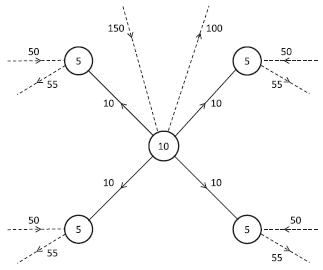
\includegraphics[width=10cm]{fig1_networkExample.png} %
%\end{center}
%\end{figure}

\begin{figure}
\par
\begin{center}
\begin{tikzpicture}[xscale=.5, yscale=.5]

\draw (5, 5) circle [radius=1];
\node at (5,5) {$10$};
\draw (10, 10) circle [radius=1];
\node at (10,10) {$5$};
\draw (10, 0) circle [radius=1];
\node at (10,0) {$5$};
\draw (0, 10) circle [radius=1];
\node at (0,10) {$5$};
\draw (0, 0) circle [radius=1];
\node at (0,0) {$5$};

\draw[dashed, -<-] (-1, 10) -- (-4, 10);
\draw[dashed, ->-] (-.7071, 9.2929) -- (-2.82843, 7.171573);
\node [below] at (-2.5, 10) {\footnotesize $50$};
\node [right] at (-1.76777, 8.232233) {\footnotesize $55$};

\draw[dashed, -<-] (-1, 0) -- (-4, 0);
\draw[dashed, ->-] (-.7071, -.7071) -- (-2.82843, -2.82843);
\node [below] at (-2.5, 0) {\footnotesize $50$};
\node [right] at (-1.76777, -1.76777) {\footnotesize $55$};

\draw[dashed, -<-] (11, 10) -- (14, 10);
\draw[dashed, ->-] (10.7071, 9.2929) -- (12.82843, 7.171573);
\node [below] at (12.5, 10) {\footnotesize $50$};
\node [left] at (11.76777, 8.232233) {\footnotesize $55$};

\draw[dashed, -<-] (11, 0) -- (14, 0);
\draw[dashed, ->-] (10.7071, -.7071) -- (12.82843, -2.82843);
\node [below] at (12.5, 0) {\footnotesize $50$};
\node [left] at (11.76777, -1.76777) {\footnotesize $55$};

\draw[dashed, -<-] (4.2929, 5.7071) -- (3.75, 12);
\draw[->-] (4.2929, 5.7071) -- (.7071, 9.2929);
\draw[dashed,  ->-] (5.7071, 5.7071) -- (6.5, 12);
\draw[->-] (5.7071, 5.7071) -- (9.2929, 9.2929);
\draw[->-] (4.2929, 4.2929) -- (.7071, .7071);
\draw[->-] (5.7071, 4.2929) -- (9.2929, .7071);
\node [left] at (4, 9) {\footnotesize $150$};
\node [left] at (6, 9) {\footnotesize $100$};
\node [left] at (3, 7) {\footnotesize $10$};
\node [right] at (7, 7) {\footnotesize $10$};
\node [left] at (3, 3) {\footnotesize $10$};
\node [right] at (7, 3) {\footnotesize $10$};
\end{tikzpicture}

\end{center}
\caption{\textbf{A simple network}. Nodes are financial institutions. There is a connection from node $i$ to node $j$ if $i$ is a net borrower from $j$. The dashed lines show connections to the outside sector.}
\label{fig:networkExample}\vspace{.3in}
\end{figure}


In addition to its claims inside the network, the central node has lent $150$ and has borrowed $100$ from the outside sector, depicted by the dashed lines with arrows going into and out of the central node. We refer to positive claims with respect to the outside sector as \textit{outside assets} and to negative claims as \textit{outside liabilities}. Outside assets typically consist of securities, loans to firms and households (including mortgages), and public debt. Outside liabilities mostly involve deposits and lines of credit.

The difference between all assets and all liabilities gives each node's net worth. The central node has a net worth of $10$, shown inside the circle that represents the node.  Each of the peripheral nodes has outside assets of $50$, outside liabilities of $55$ and an inside asset of $10$ with respect to the central node, for a net worth of $5$.

\subsection{Shocks and Propagation}

The shocks we consider are exogenous reductions in the value of outside assets. Therefore, all initial losses always originate outside the network. One example of such a shock is an increase in defaults for residential mortgages held by financial institutions.

For sufficiently high initial losses in outside assets, some nodes in the network will be unable to pay their creditors in full. When this happens, all debts for the defaulting node (including those outside the network) are written down pro rata and creditors receive only a fraction of their promised payments. Note that under a pro rata allocation, a node defaults on either all of its creditors or none of them. When creditors for some node are not paid in full, they may themselves be unable to pay their own creditors, and so on. Initial losses thus get transmitted inside the network through this ``domino'' effect. We do not include in our analysis any liquidity or equity injections, and only net claims between two nodes are assumed to be of relevance (as opposed to gross positions). In addition, nodes do not renegotiate claims, even if it may be mutually beneficial to do so.

As a numerical example, consider what happens when the outside assets of the central node in Figure \ref{fig:networkExample} receive a shock of size $80$. Outside assets for the central node decrease from $150$ to $70$. Total liabilities are initially $140$. After the shock, under a pro rata allocation, only $50$ percent of each liability is repaid as the central node only has $70$ remaining in assets. Each of the peripheral nodes receives $5$ from the central node, just enough to balance their assets and liabilities. A shock to the outside assets of the central node of magnitude greater than $80$ would reduce the value of assets for peripheral nodes below the value of their liabilities. In this case, the peripheral nodes would default on their creditors. In this case, the central node has created contagion to the peripheral nodes through network contagion. The peripheral nodes default even though none of their outside assets were affected by the initial shock.

\subsection{The Disconnected Network}

To quantify the amplification of losses stemming from the network structure --as opposed to the initial losses from exogenous shock to outside assets-- we compare expected losses for the system (the network plus the outside sector) to the losses in a hypothetical system in which all connections inside the network have been severed. Both networks are subject to the same distribution of exogenous shocks to outside assets, and to no other shocks. We create this hypothetical \textit{disconnected} system by removing all connections between nodes inside the original network but keeping the links with the outside sector intact. We also assume the net worth at each node remains unchanged by creating, for each node, a fictitious claim to the outside sector equal in value to the net value of all the connections that were removed. Depending on the sign of the net value of removed connections, the new fictitious claim can be an asset or a liability. If it is an asset, we assume it is not subject to the shocks to outside assets to keep the set of assets initially shocked identical to that of the original network. If the new fictitious claim is a liability, we assume it has the same priority as all other liabilities. In case of default, the new fictitious liability gets haircut pro rata just like all other non-fictitious liabilities, and any ``losses'' imposed on that obligation are counted towards the value of total system losses. Figure \ref{fig:disconnectedNetwork} shows the disconnected version of network displayed in Figure \ref{fig:networkExample}.

\begin{figure}
\par
\begin{center}
\begin{tikzpicture}[xscale=.5, yscale=.5]

\draw (5, 5) circle [radius=1];
\node at (5,5) {$10$};
\draw (10, 10) circle [radius=1];
\node at (10,10) {$5$};
\draw (10, 0) circle [radius=1];
\node at (10,0) {$5$};
\draw (0, 10) circle [radius=1];
\node at (0,10) {$5$};
\draw (0, 0) circle [radius=1];
\node at (0,0) {$5$};

\draw[dashed, -<-] (-1, 10) -- (-4, 10);
\draw[dotted, -<-] (-1, 10) -- (-4, 11.5);
\draw[dashed, ->-] (-.7071, 9.2929) -- (-2.82843, 7.171573);
\node [below] at (-2.5, 10) {\footnotesize $50$};
\node [right] at (-1.76777, 8.232233) {\footnotesize $55$};
\node [above] at (-2.5, 11) {\footnotesize $10$};

\draw[dashed, -<-] (-1, 0) -- (-4, 0);
\draw[dotted, -<-] (-1, 0) -- (-4, 1.5);
\draw[dashed, ->-] (-.7071, -.7071) -- (-2.82843, -2.82843);
\node [below] at (-2.5, 0) {\footnotesize $50$};
\node [right] at (-1.76777, -1.76777) {\footnotesize $55$};
\node [above] at (-2.5, 1) {\footnotesize $10$};

\draw[dashed, -<-] (11, 10) -- (14, 10);
\draw[dotted, -<-] (11, 10) -- (14, 11.5);
\draw[dashed, ->-] (10.7071, 9.2929) -- (12.82843, 7.171573);
\node [below] at (12.5, 10) {\footnotesize $50$};
\node [above] at (12.5, 11) {\footnotesize $10$};
\node [left] at (11.76777, 8.232233) {\footnotesize $55$};

\draw[dashed, -<-] (11, 0) -- (14, 0);
\draw[dotted, -<-] (11, 0) -- (14, 1.5);
\draw[dashed, ->-] (10.7071, -.7071) -- (12.82843, -2.82843);AH
\node [below] at (12.5, 0) {\footnotesize $50$};
\node [above] at (12.5, 1) {\footnotesize $10$};
\node [left] at (11.76777, -1.76777) {\footnotesize $55$};

\draw[dashed, -<-] (4.2929, 5.7071) -- (4, 12);
\draw[dashed, ->-] (5.7071, 5.7071) -- (6, 12);
\draw[dotted, ->-] (5.7071, 5.7071) -- (8, 12);
\node [left] at (4.25, 9) {\footnotesize $150$};
\node [left] at (6, 9) {\footnotesize $100$};
\node [right] at (6.5, 8) {\footnotesize $40$};

\end{tikzpicture}

\end{center}
\caption{\textbf{A Simple Disconnected Network}. The disconnected version of 
the networks in Figure \ref{fig:networkExample} are obtained by
removing all connections between nodes inside the original network but
keeping the links with the outside sector intact. Net
worth remains unchanged by creating fictitious outside assets or liabilities. Dashed lines indicate actual balance sheet assets and liabilities, and dotted lines indicate fictitious assets from or liabilities to the outside sector.}
\label{fig:disconnectedNetwork}\vspace{.3in}
\end{figure}

\subsection{An Upper Bound on Network Spillovers}

We are interested in whether the expected system losses in our real-world, interconnected system are substantially greater than those in the hypothetical \textit{disconnected} system, where node connections have been excised. We define $R$ to be the ratio of expected losses for the actual network to the expected losses in the disconnected network. That is, if $L$ denotes total system losses,

\begin{equation}
R=\frac{E(L_{\text{Actual}})}{E(L_\text{Disconnected})}
\end{equation}


The value of $R$ gives the relative magnitude of additional losses imposed on the system because of the interconnected structure of the network - to wit, network effect losses. With perfect information on the bilateral claims in the system, this ratio could be calculated exactly in response to a variety of shocks by using the \citet{eisenberg2001systemic} algorithm to compute the set of node payments that `clear' the system (i.e. follow the system's rules of limited liability and pro rata allocation). In the United States financial system, detailed and publicly-available data on bilateral obligations between financial firms does not exist. 

The main result in \citet{glasserman2015likely} is that a useful upper-bound on $R$ can be derived without any information on the makeup of each node's bilateral claims. We call this upper-bound $B$. If the tails of the distribution of exogenous shocks to outside assets are not too fat-tailed, then $B$ can be calculated using node-specific information only\footnote{More technically, we consider shocks that have an \textquotedblleft increasing failure rate" (IFR). A random variable with distribution function  $G\left( x\right) $ and density $g\left( x\right) $ is said to have an IFR if $g\left( x\right) /(1-G\left( x)\right) $ is an increasing function of $x$ . This family encompasses the normal, exponential, and uniform distributions. There are no restrictions on the correlation structure of shocks.  \par In addition, the joint distribution of potential shocks is assumed to be invariant to scale (homogeneous in assets). For example, if total assets of a node double, expected losses are assumed to also double.}. \citet{glasserman2015likely} show that $B$ depends only on each node's total outside assets $c$, each firm's probability of default due to direct shocks to outside assets $\delta$, and the maximum \textit{liability connectivity} among nodes in the system $\beta^+$. Each node's liability connectivity is defined as its ratio of inside liabilities to total liabilities.

\citet{glasserman2015likely} show that

\begin{equation} \label{eq:B}
B=1+\frac{1}{(1-\beta ^{+})}\frac{\sum_{i \in S} {\delta _{i}c_{i}}}{\sum_{i \in S}{c_{i}}},
\end{equation}

\begin{eqnarray*}
\delta _{i} &:&\text{probability of default from outside shocks for node }i, \\
c_{i} &:&\text{the dollar value of outside assets for node }i, \\
\beta ^{+} &:&\text{maximum liability connectivity, i.e., }\beta^{+}=\max_{i \in S}\beta _{i}\text{, with } \beta_i=\text{the fraction of } \\
&& \text{firm i's liabilities held by other nodes in the networks}, \\
S &:&\text{Set of financial institution nodes within the network.}
\end{eqnarray*}%

The upper bound $B$ for network spillovers is increasing in the maximum financial connectivity of the system, $\beta ^{+}$, and in the quantity $\sum {\delta _{i}c_{i}}/\sum {c_{i}}$, most-easily interpretable as a weighted average probability of default for the system (with each firm's weight given by its share of total outside assets). When $\beta ^{+}$ is close to $1$, aggregate financial connectivity is high and any initial shock to outside assets has the potential to be transmitted broadly across the network. In contrast, when $\beta ^{+}$ is close to zero, any initial shock dissipates quickly and expected losses should be similar to those in a truly disconnected network.

For most systems calibrated to real-world data, previous studies have found that the upper bound $B$ is small. For example, picking $\beta ^{+}=0.8$ and $\delta _{i}=1$ percent for all nodes $i$, we get $B=1+0.01/(1-0.8)=1.05$. This means that the connected system has expected losses that are at most $5$ percent larger than those in the system of isolated nodes. In their example exercise, \citet{glasserman2015likely} find an even smaller upper bound of $1.0175$ for European banks using data from the the 2011 European Banking Authority stress test.

\subsection{The Network Vulnerability Index}

We define the \emph{Network Vulnerability Index} (NVI) to be the upper bound on the magnitude of additional expected losses created in the system by network spillovers, expressed as a share of expected disconnected system:

\begin{equation} \label{eq:NVI}
NVI=\left( B-1\right) = \frac{1}{(1-\beta ^{+})}\frac{\sum {\delta _{i}c_{i}}}{\sum {c_{i}}}.
\end{equation}

Being an upper bound, the $NVI$ is most useful when its value is small, since the model then clearly indicates low vulnerability to potential network spillovers. When the index is large it is less informative. In this case, the true value of potential network spillovers could be as large as the upper bound or as low as zero, as dictated by the bilateral claims between nodes. The model does not produce any additional information that can help pinpoint the true value of network spillovers within that the range $\left[ 0,NVI\right] $. As an extreme, when the $NVI$ is equal to infinity, it provides no information\footnote{In this section, we have used the words ``small'' and ``large'' to characterize different levels of the $NVI$ without being explicit about their meaning. This was a deliberate choice, since the model provides no welfare analysis and no other indication on how to evaluate the overall magnitude of the $NVI$. In short, the burden of interpreting what constitutes small or large values for the $NVI$ is the policymaker's.}.

\subsection{A Firm-Specific Risk Measure: The `Contagion Index'}

\citet{glasserman2015likely} also presents a firm-specific measure of the potential to cause contagion, which they term a firm's `contagion index'. For a wide family of shocks, the index is defined as 

\[\text{contagion index} = w_i \beta_i \lambda_i\]

\noindent where $w_i$ is a firm's net worth, $\beta_i$ is liability connectivity as in equation \ref{eq:NVI}, and $\lambda_i=\frac{c_i}{w_i}$ is the leverage of firm $i$'s outside assets. 

Given that the magnitude of exogenous shocks to outside assets in the model is bounded by each firm's actul quantity of outside assets, the contagion index calculates the total payment shortfall that a firm could potentially pass on to other nodes following a shock to its own outside assets. \citet{glasserman2015likely} show that an outside asset shock to node $i$ cannot possibly cause default to node $j$ if node $j$'s net worth is greater than node $i$'s contagion index. They also show that the \textit{probability} of node $j$ defaulting solely because of a shock to node $i$'s assets \textit{must} be less than the probability of node $j$ defaulting from a shock to its own assets if $i$'s contagion index is less than $j$'s quantity of outside assets, $c_j$\footnote{The bounds derived by \citet{glasserman2015likely} are actually stronger than this - applying to the probability of node $i$ causing default through contagion to a given \textit{group} of firms.}.

\section{Data and Empirical Methodology}
\label{sec:data}

This paper combines a number of different data sources to estimate the fields in equation \ref{eq:NVI}. What follows is a description of those data sources and any decisions made in how to best utilize them. The resulting datasets yields a quarterly series for the NVI spanning 2002:Q1 to 2016:Q4.

\subsection{Assets and Liabilites of Bank Holding Companies}

Line-item balance sheet information for bank holding companies comes from quarterly filings of the Federal Reserve's FR-Y9C reporting form\footnote{An FR-Y9C filing is required by each domestic bank holding company (BHCs), savings and loan holding company, US intermediate holding company, and securities holding company with total assets exceeding one billion dollars}. The public nature of this data, as well as the level of granularity in reported asset and liability classes, make this form particularly well-suited to our analysis.

Our objective in using FR-Y9C data is to estimate the outside assets and liability connectivity of each firm in the FR-Y9C's sample. This involves classifying each of the form's asset and liability line items as \textit{inside} or \textit{outside} the financial system. We produce this classification for each of the line items in the current FR-Y9C balance sheet, and apply those classifications across each firm in the sample\footnote{The `current' iteration of the form used in this paper is that from December 2016. For brevity, we will continue to refer to this as the `current' form.}. In cases where this binary classification seems inappropriate, we split the value of the field, classifying fifty percent of its magnitude as inside the system and fifty percent as outside the system\footnote{Section \ref{sec:robustness} shows that our estimates are not very sensitive to alternative assumptions about the share of inside and outside assets and liabilities in these more ambiguous categories.}. The final two columns of Tables \ref{tab:assets_y9c} and \ref{tab:liabilities_y9c} provide these classification breakdowns for current variables (or groups of variables) in the form. 

In past versions of the form, line-items were often less granular. To apply our inside-vs-outside classifications (made based on the current form's line-items) backward to previous form versions, we find the variables in each past form that include the same assets or liabilities as a given group of variables in the current form (the latter group of variables is typically larger, reflecting a movement towards. increasing form granularity over time). We then compute a firm-specific percentage of the total value of the current-form variable group that is attributable to each individual variable in the group during the first year that the variable group was reported\footnote{To consider a simple but illustrative example - say we have determined that the asset categories contained in variables Y1 and Y2 of the current form are the same as those in variable X from some earlier version of the form. We then define $P_{Y1,i}$ and $P_{Y2, i}$ for firm i as the average of $\frac{Y1_i}{Y1_i+Y2_i}$ and $\frac{Y2_i}{Y1_i+Y2_i}$ in the first year that both Y1 and Y2 are reported. Firm i's imputed values for Y1 and Y2 in the early sample then becomes $P_{Y1,i}X$ and $P_{Y2, i}X$.}. By applying this estimated share back through time to 2002, we create a series for each FR-Y9C variable that is roughly consistent over time\footnote{In practice, these breakdowns are only important when the group of current-form variables includes two or more different in-vs-out classifications. Otherwise, the total sum of variables is directed into the same categorization, and any variable-by-variable divisions within the total sum become irrelevant.}. For a detailed view of the current-form variable groups identified, and the method used to extend them back to 2002, see Tables \ref{tab:assets_y9c} and \ref{tab:liabilities_y9c}.

\subsection{FDIC-Insured Deposits of BHCs}\label{subsec:Deposits}

We wish to avoid classifying any FDIC-insured deposits from the commercial bank subsidiaries of BHCs as inside the financial system, since those deposits are likely not held by financial firms and are ultimately government liabilities (which reside outside the network). To separate FDIC-insured deposits from a BHC's total deposits, we use quarterly data from the FFIEC 041 (also known as the Call Report), as collected by the Federal Financial Institutions Examination Council\footnote{More specifically, our primary variables of interest from the form are RCON2200 (total domestic deposits) and RCON5597 (estimate of uninsured domestic deposits). Our estimate of insured deposits becomes the difference between these two fields. It is worth noting that our final estimate of uninsured deposits (which is then used in our index) is the difference between this estimate of insured deposits and the FR-Y9C form's value for firm domestic deposits (\textit{not} the Call Report's domestic deposits variable). It is our understanding that the FR-Y9C form, as it pertains to entire BHCs instead of just commercial bank subsidiaries, includes a better estimate of total deposits for our purposes.}. After matching each commercial bank to its BHC parent, we subtract the estimated quantity of FDIC-insured deposits, as reported in the Call Report, from the BHC's total deposits. Only this final ``uninsured'' value of deposits is considered inside the financial system, for the purposes of further analysis\footnote{In our benchmark setup for the NVI, 100\% of uninsured domestic deposits are counted as \textit{inside} the system. While this is likely close to accurate for the custodian banks (banks whose deposits are primarily safeguards of the assets of other banks) in our sample -- namely State Street and Bank of New York Mellon -- this is certainly unrealistic for many of the other BHCs in our panel. Section \ref{sec:robustness} includes robustness exercises on different configurations, including one allowing for more firm-specific allocation percentages. In short, this decision makes little difference in our final NVI series.}.

The process of matching Call Report data to balance sheet data on its BHC parent can become complicated, particularly around BHC mergers, acquisitions, or legal classification changes. To find the final BHC parent of each commercial bank, we use a bank-parent matching hierarchy maintained by the Federal Reserve Bank of New York. We then match commercial banks to their parent BHCs based on the BHC's RSSID identifier code. When this process does not lead to any commercial bank matches for a given BHC, we then match that BHC to all the commercial banks owned by the BHC's parent organization. This can occassionally lead to overestimates of the FDIC-insured deposits of these BHCs, but we have found that this process almost always yields sensible-looking series for these BHCs' financial connectivities. The alternative approach, where we do not conduct the second matching procedure and list FDIC-insured deposits as `0' for these firms, often yields impractically-large financial connectivities.  

\subsection{Probabilities of Default}

The probabilities of default $\delta$ for each firm in equation \ref{eq:NVI} are the true - or physical - probabilities of default. As such, any risk-neutral estimate of a firm's default probability (such as those commonly extracted from credit default swaps or corporate bond spreads) would be inappropriate for calculating our NVI.

We consider Moody's Analytics' (formerly KMV's) Expected Default Frequency (EDF) series to be suitable for our analysis. The EDF measure uses typical lognormal assumptions and an options-pricing approach to equities to determine which variables should theoretically be important for determining a given firm's probability of default. They then use them to fit an empirical model of default probabilities using Moody's extensive database of historical defaults, as explained in \citet{kmv_methods}\footnote{Moody's historical defaults dataset considers government rescues as default events, if the rescue specifically saved the firm from default. So, in that sense, the EDF series can be considered as a probability of default without government intervention. As the model of \citet{glasserman2015likely} does not include the possibility of government rescue, this empirically estimated probability closely matches its model counterpart.}.

Equation \ref{eq:NVI} calls for the probability of default due to shocks to outside assets, although Moody's Analytics' EDF makes no distinction between the actual sources of default losses. Rather than attempt to back out the theoretically-appropriate default probability from these EDFs, we simply include the EDF value itself as $\delta_i$ for each firm in equation \ref{eq:NVI}, with the understanding that this probability is in fact an upper-bound on the direct default probability. Relying on the fact that the NVI is itself an upper-bound, the bounds obtained from an NVI calculated this way will still be valid. 

Moody's EDF model produces a daily series of physical expected default frequencies at one-year horizons. We define a firm's quarterly EDF measure to be the average of its daily measures over a given quarter.

\subsection{Non-BHC Financial Firms} \label{subsec:non_bhc}

For financial firm subsectors whose firms do not file FR-Y9C forms, we include nodes into the NVI using less granular firm-level balance sheet information and subsector-level data on assets and liabilities from the Financial Accounts of the United States, maintained by the Board of Governors of the Federal Reserve System.

To incorporate a new firm (or, in this case, group of firms) into our NVI measure requires us to know each firm's individual default probability $\delta_i$, its outside assets $c_i$, and that firm's liability connectivity $\beta$ \textit{if} that firm's $\beta$ becomes the new $\beta^+$ for the system. We first make the necessary simplifying assumption that the $\beta^+$ selected from the firms in our FR-Y9C sample correctly identifies the $\beta^+$ for the entire network\footnote{In fact, the $\beta^+$ we select from the FR-Y9C sample for the NVI is the highest financial connectivity found in the top 20 BHCs by assets. See \ref{sec:robustness} for a discussion of this decision, and an analysis of robustness to different selections.}.

Left to determine is how the inclusion of other financial subsectors affects the other component of the NVI, the weighted average default probability $\frac{\sum {\delta _{i}c_{i}}}{\sum {c_{i}}}$. We approximate the value of this componenet for the subsectors not covered by the FR-Y9C by first constructing an estimate of the total outside assets of each of those subsectors from the Financial Accounts of the United States and then computing an average default probability weighted by assets for each new subsector using total firm asset values and Moody's EDF measures. Total quarterly assets for each firm, compiled from that firm's financial releases and filings, are also available in the Moody's EDF dataset\footnote{This is done using a method similar to that for the FR-Y9C, categorizing different Financial Accounts asset classes as inside or outside the system. See Table \ref{tab:ffunds_inout} for the precise `inside' vs `outside' classification used for different variables in the release. Line-items from the Financial Accounts are much coarser than those in the FR-Y9C, making this an admittedly cruder method of classification. As Section \ref{sec:robustness} shows, however, this breakdown has very little effect on the final NVI measure.}.

More explicitly, let $Y$ denote the set of firms in our FR-Y9C sample, $S = \{S_1, S_2, \cdots\}$ denote a set of sets, with each individual element $S_j$ being the set of firms belonging to some new financial subsector, and let $A$ denote the entire financial network $Y \cup S$. Then, 
\begin{equation}\label{eq:approx}
\frac{\Sigma_{A} \delta_i c_i}{\Sigma_A c_i} = \frac{\Sigma_Y \delta_i c_i+ \Sigma_{S_j \in S}(\Sigma_{i \in S_j } \delta_ic_i)}{{\Sigma_Y c_i}  + \Sigma_{S_j \in S}(\Sigma_{i \in S_j}c_i)} \approx \frac{\Sigma_Y \delta_i c_i+ \Sigma_{S_j \in S}(\bar{\delta_{S_j}}\Sigma_{i \in S_j} c_i)}{{\Sigma_Y c_i} + \Sigma_{S_j \in S}(\Sigma_{i \in S_j}c_i)} 
\end{equation}
\begin{equation}
\text{where } \bar{\delta_{S_j}} = \frac{\Sigma_{i \in S_j} \delta_i a_i}{\Sigma_{i \in S_j}a_i}, \text{with } a = \text{total assets of firm i} \label{eq:avg_def}
\end{equation}
This computation is only an approximation of the true $\frac{\Sigma_{A} \delta_i c_i}{\Sigma_A c_i}$ for two reasons. First, the weighted average probability of default per sector $\bar{\delta_{S_j}}$ is weighted here by \textit{total assets} per firm, where a more precise measure for the NVI would be weighted by \textit{outside assets} per firm. Second, and more significantly, our sample of average default probability is limited to those firms for which we have a Moody's EDF measure - namely, to publicly-traded firms. Provided that our computed averages are good representations of the entire sector, then the NVI constructed using this approximation should remain a useful upper-bound on network spillovers that allows us to include a much larger portion of the US financial system than the FR-Y9C sample alone would allow.

\subsection{Subsector EDF Samples}

Per Section \ref{subsec:non_bhc}, we wish to include subsector-wide averages in our NVI for security broker dealers, insurance companies, real estate investment trusts, and an `other' category for several other types of financial firms. To determine which firms should comprise each subsector's sample in equation \ref{eq:avg_def}, we use Moody's Analytics' own internal sectoral classification system, pairing their categorizations with the subsector definitions given in the Financial Accounts of the United States. For the purposes of calculating outside assets $c$ for the `other' sector, we sum across the Financial Accounts subsectors for credit unions, finance companies, funding corporations, and issuers of asset-backed securities\footnote{The `other' category is the only one for which finding an appropriate subsample within the EDF dataset it not straightforward. We choose to include any firms with sectoral tags of `Finance Companies', `Investment Management', or `Finance Not Elsewhere Classified' in this node's average probability calculation.}.

To show the relative magnitude of assets assigned to these difference subsectors by the Financial Accounts of the United States, we plot the percentage of total network assets (defined as the sum of total financial assets in each subsector described above, plus the Financial Accounts' total financial assets for BHCs) attributable to each of these subsectors in Figure \ref{fig:ffunds_assets}. As Figure \ref{fig:ffunds_assets} shows, BHCs are by far the largest financial subsector by assets, meaning that the weights given to BHCs' default probabilitys will, in aggregate, be larger than the weights assigned to any of the included subsectors.  

\begin{figure}
\begin{center}
\includegraphics[width = \textwidth]{../output/ffunds_assets_area.pdf}
\end{center}
\caption[]{\textbf{Total Financial Assets for each Network Subsector, as a Percentage of Total Network Assets.} According to the Financial Accounts of the United States, BHCs comprise by far the largest percentage of network assets}\label{fig:ffunds_assets}
\end{figure}

%\begin{figure}
%\begin{center}
%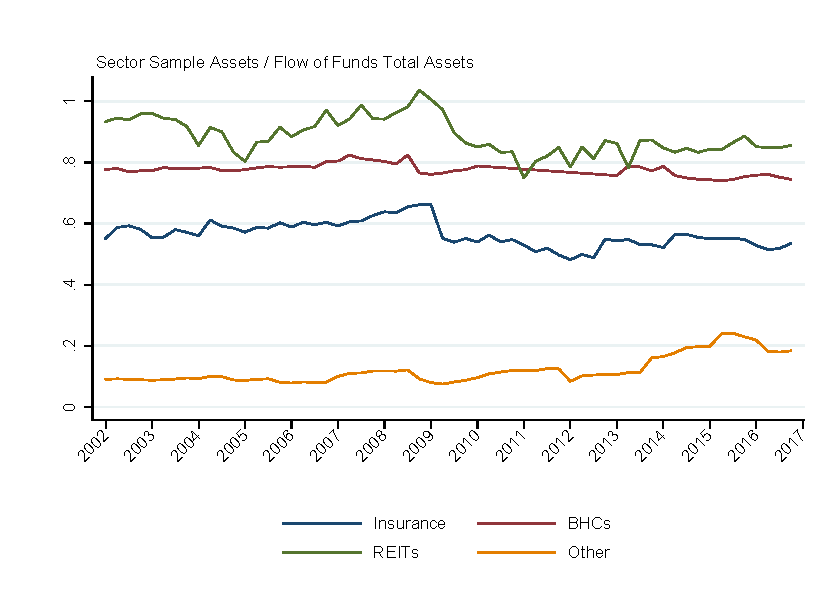
\includegraphics[width = \textwidth]{../output/coverage.pdf}
%end{center}
%\caption[]{\textbf{Data Coverage of Compustat Subsample.} Only a subsample of firms in each subsector are available to calculate a sector-wide probability of default, which is then used to approximate our network vulnerability measure for a network including these subsectors. The percent of sector assets covered for insurance companies and bank holding companies is relatively high and stable. Data coverage for broker-dealers is very high before the financial crisis, then drops. Real estate investment trusts are well-covered by the EDF dataset, while the umbrella category of `other' is not.}\label{fig:coverage}
%\end{figure}

\begin{figure}
\begin{center}
\includegraphics[width = \textwidth]{../output/coverage_broad.pdf}
\end{center}
\caption[]{\textbf{Data Coverage of EDF Sample for NVI, Against Total Network Assets.} Only a subsample of firms in each subsector have their default probabilities directly enter the NVI. The first line sums the total assets of firms whose EDF measures enter the NVI in some form - either individually if that firm filed an FR-Y9C, or as part of a subsector average default probability sample - divided by total network assets from the Financial Accounts of the United States. The second line plots the same, if we instead consider each approximated subsector node per equation \ref{eq:approx} to cover the entire sum of that subsector's assets.}\label{fig:coverage_broad}
\end{figure}

To assess whether the samples used to compute each of the default probabilities within equation \ref{eq:approx}, in Figure \ref{fig:coverage_broad} we plot the percentage of total network assets (with the `network' defined as the sum of total financial assets in the subsectors of Figure \ref{fig:ffunds_assets}) that are accounted for by the total assets of firms whose default probabilities directly enter into the NVI - either individually if that firm files an FR-Y9C, or as part of the sample for computed a subsector's average default probability. The red line in Figure \ref{fig:coverage_broad} plots the same value, if we consider each approximated node in equation \ref{eq:approx} to cover all of the assets from that subsector's Financial Accounts entries. The blue line shows that even the most conservative measure covers consistently more than 50\% of the assets of the entire U.S. financial system. If we consider our network to cover the sectors of each approximated subsector node, that coverage becomes even higher, as shown in the red line of Figure \ref{fig:coverage_broad}\footnote{Note that the actual assets attributed to each subsector for the purposes of calculating these coverage statistics are total subsector assets \text{after} any deductions from FR-Y9C sample overlap. This adjustment, as well as the fact that FR-Y9C coverage of BHC assets in the Financial Accounts is not 100\%, are why the second line in Figure \ref{fig:coverage_broad} is not mechanically 100\%.}.


%$\bar{\delta_{S_j}}$ cover a reasonably-wide array of each subsector's assets, we plot the share of total sector assets (computed from the Financial Accounts of the United States) that are accounted for by the subsample of firms used to calculate the average sector default probabilities. The results of this exercise are presented in Figure \ref{fig:coverage}\footnote{See \ref{sec:appendixb} for a discussion of why coverage for broker dealers is low, and why we do not believe this is cause for major concern in our estimate.}.

%The coverages of our insurance company subsample and our Y9C sample (the denominator for which is the sum of total assets in `private depository institutions' and `holding companies' from the Flow of Funds) are both relatively high and reasonably stable over our sample period. The coverage for security brokers and dealers is very high before the financial crisis, but then drops precipitously. To understand why this occurs, and why we do not believe it is cause for concern, we also show \Cref{fig:dealer_coverage_details}, which compares the timing of that drop with several large-scale acquisitions and firm classification changes around that time. The drops in dealer coverage exactly coincide with acquisitions of broker dealer firms by BHCs included in our FR-Y9C sample, as evidenced by the spikes in assets of JP Morgan and Bank of America at the same times as coverage drops. Low coverage is further exacerbated by the inclusion of Goldman Sachs and Morgan Stanley in the FR-Y9C sample at the same time. When a firm is included in the FR-Y9C sample, it is \textit{excluded} from the subsample of sector firms used to calculate that sector's average probability of default (and its assets are also excluded from that sector's estimate of total outside assets, also used in the NVI). Thus, the low `coverage' of broker-dealers later in the sample is not a result of assets being excluded from the sample - but rather a shift in categorization of certains firms from subsamples $B$ to $Y$, to use the nomenclature above.


\subsection{Defaulting firms}

The model of \citet{glasserman2015likely} includes an explicit assumption that no nodes included in the system are initially in default (defined as having book liabilities greater than book assets). To avoid including any such firms in our estimates of equation \ref{eq:approx}, we use Moody's Analytics' Default and Recovery Database to identify dates of bankruptcy filing. If a firm files for bankruptcy at any point during our sample period (2002-Q1 to 2016-Q4), then no expected default frequency data is used for that firm after the date of filing.

\section{Results}
\label{sec:results}

\subsection{Network Vulnerability Index Estimates}

Figure \ref{fig:NVI_benchmark} plots the NVI --- the upper bound on expected network default spillovers. The figure shows the main result of our paper: When estimated empirically, vulnerability to network spillovers can range from negligible to large. 

\begin{figure}[h!]
\begin{center}
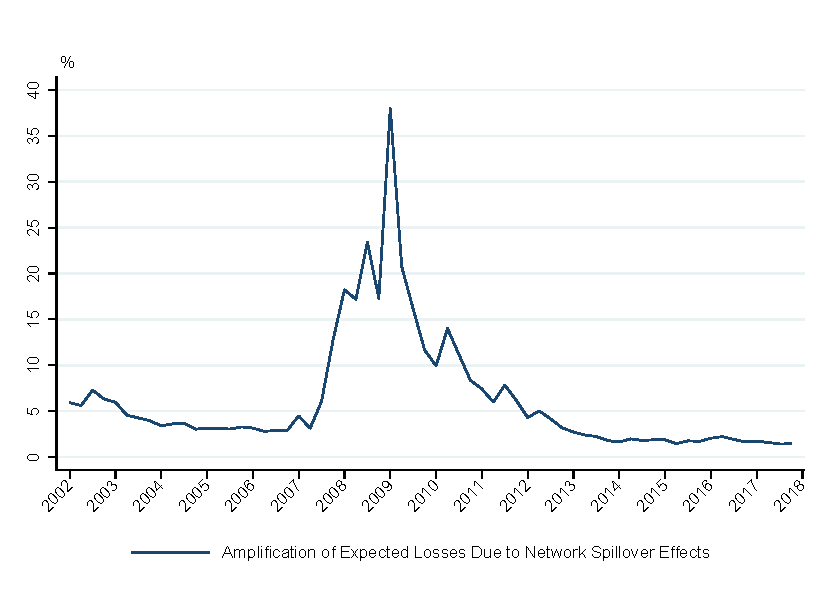
\includegraphics[width = \textwidth]{../output/NVI_benchmark.pdf}
\end{center}
\caption[]{\textbf{Network Vulnerability Index (NVI).} The NVI is an upper bound on expected losses due to default network spillovers in the U.S. financial system, expressed as a share of initial (exogenous) losses to assets outside the network. Between 2008 and 2012, network default network spillovers amplified expected losses by between 5 and 25 percent.} \label{fig:NVI_benchmark}
\end{figure}

The NVI was essentially zero from 2002-Q1 to 2007-Q4, with only a slight increase in 2007-Q3 and 2007-Q4, which immediately implies that expected vulnerability to network default spillovers were negligible for this period. Contrary to some narratives of the crisis, we do not observe any substantial buildup of network fragility of the kind we study in the years leading up to the crisis. To understand this result, we decompose our spillover measure into two factors: the weighted average of probabilities of default ($\frac{\Sigma \delta_i c_i}{\Sigma c_i}$) and a `connectivity multiplier' ($\frac{1}{1-\beta^+}$) that captures the magnitude with which initial losses in outside assets can be transmitted and amplified through network connections. The final NVI measure is the product of these two components. 

As Figure \ref{fig:NVI_components} shows, both factors contribute to the low spillover measure in the period 2002-Q1 to 2007-Q4. Because probabilities of default were miniscule in this period, the weighted average default probabilities were close to zero. Since Moody's EDF  probabilities are physical, they are adjusted for risk and thus unlikely to arise because of any low risk premium observed during this period\footnote{In addition, version 9 of KMV generally adjusts probabilities of default (upwards) for this period taking into account the ex-post defaults observed during the crisis that were not expected before it, minimizing the concern that our results are driven by any potential underestimation of default probabilities before the crisis.}. Over the same period, the connectivity multiplier declined by 10 percent. Thus, neither the vulernability of firms to default nor the inner topology of the financial network signaled any increased vulnerability.

\begin{figure}[h!]
\begin{center}
\includegraphics[width = \textwidth]{../output/NVI_components.pdf}
\end{center}
\caption[]{\textbf{NVI Decomposition.} The NVI is the product of the asset-weighted probability of default of firms inside the network and a ``connectivity multiplier'' that captures the degree of amplification and transmission created by defaults inside the network..} \label{fig:NVI_components}
\end{figure}

During the height of the crisis, between 2008-Q1 and 2008-Q4, outside assets (especially real estate) experienced sharp declines in realized and future expected values, pushing up our measure of spillovers. The connectivity multiplier, in contrast, was a mitigating factor, as it noticeably declined, reflecting financial institutions’ desire to reduce their counterparty exposure to each other in times of stress. In fact, the decline in the connectivity multiplier over 2008 was as large as the decline observed over the six preceding years 2002-2007. Figure \ref{fig:betas} shows $\beta^+$, the maximum liability connectivity selected at each point of the sample, which drives this dynamic. Overall, in late 2008 the increase in default probabilities outweighed any mitigation from lower connectivity. Our estimates indicate that expected network default spillovers over this period could amplify total initial losses by at most 11.4 percent. Whether 11.4 percent should be considered a small or large number is in the eye of the beholder.

\begin{figure}[h!]
\begin{center}
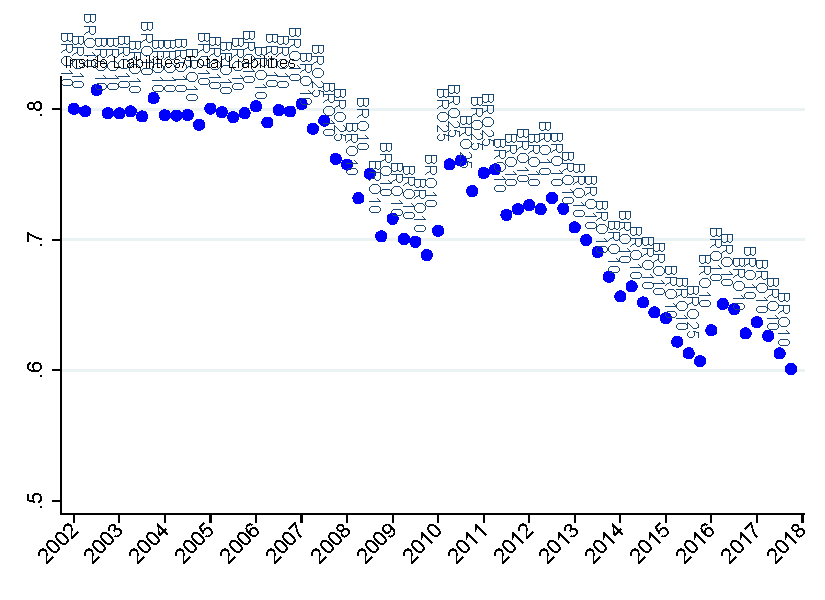
\includegraphics[width = \textwidth]{../output/connectivities_1.pdf}
\end{center}
\caption[]{\textbf{Maximum Liability Connectivity Among Large BHCs ($\beta^+$)}. The most interconnected BHC before the financial crisis was JP Morgan \& Chase. After Goldman Sachs and Morgan Stanley join the BHC sample in 2009, they become the most interconnected firms for the remainder of the sample.} \label{fig:betas}
\end{figure}

In 2009-Q1, after the failure of several financial institutions and with the crisis now global in scope, the spillover measure jumped markedly, with our estimates indicating that expected network default spillovers over this period could amplify total initial losses by up to 25 percent, the largest value observed in our sample. The large increase from 2008-Q4 to 2009-Q1 was driven by both default probabilites and financial connectivity. Expected losses increased not only because real estate kept deteriorating, but also because the slowdown in real economic activity induced an increase in expected losses for almost all categories of outside assets, including commercial, industrial and consumer loans. Financial connectivity also increased, driven by the failure of some network nodes and the merger and consolidation of various other nodes. Keeping in mind that our estimates are always upper bounds and not point forecasts, to the best of our knowledge, a 25 percent amplification is the largest empirical estimate for network spillovers in the literature. Estimates that exceed 25 percent in the literature usually rely on additional amplification mechanisms (like bankruptcy costs -- see Section \ref{sec:robustness} -- or the interaction of default cascades with other phenomena, such as runs and fire-sales. The NVI remains highly elevated in 2009-Q2 at 23 percent before dropping to 18.6 percent and 12.5 percent in 2009-Q3 and 2009-Q4, respectively.

After 2009, our spillover measure hovered between 5 and 10 percent until 2012, when the European crisis started to recede. From 2013 onward, the measure steadily decreased and reached pre-crisis levels by 2015. The most important contributor to this decrease was the reduction in the probability of default of financial institutions, particularly bank holding companies that strengthened their equity capital positions substantially over this period. Financial connectivity remained elevated until 2014 and has been declining ever since. Starting in 2015, average default probabilities have slightly increased. However, because financial connectivity has continued to decline between 2015 and 2017, our overall measure of spillovers is little changed.

\subsection{Results of FR-Y9C Asset and Liability Line-Item Classifications}

Tables \ref{tab:perc_assets} and \ref{tab:perc_liabs} show what percentage of BHC inside and outside assets and liabilities are attributable to each of several broad categories of balance sheet items, based on our classifications in Tables \ref{tab:assets_y9c} and \ref{tab:liabilities_y9c}.

These being BHCs, it is unsurprising that deposits comprise a large portion of both inside and outside liabilities. Inside assets are mostly comprised of repurchase agreements, federal funds, and deposits, while outside assets are mostly loans and mortgage-backed securities.

\newpage

\begin{table} [H]\centering
\def\sym#1{\ifmmode^{#1}\else\(^{#1}\)\fi}
\begin{minipage}{.48\textwidth}
\input{../output/asset_in_formatted}
\end{minipage}%
\begin{minipage}{.48\textwidth}
\input{../output/asset_out_formatted}
\end{minipage}
\centering
\caption[]{\textbf{Shares of BHC Assets Inside and Outside the Financial System By Category, 2016-Q4.}} \label{tab:perc_assets}
\end{table}

\newpage

\begin{table} [H]\centering
\def\sym#1{\ifmmode^{#1}\else\(^{#1}\)\fi}
\begin{minipage}{.48\textwidth}
\input{../output/liab_in_formatted}
\end{minipage}%
\begin{minipage}{.48\textwidth}
\input{../output/liab_out_formatted}
\end{minipage}
\caption[]{\textbf{Shares of BHC Liabilities Inside and Outside Financial System by Category, 2016-Q4.}} \label{tab:perc_liabs}
\end{table}

\subsection{Sector-Specific Average Default Probabilities}

As we discuss in Section \ref{subsec:non_bhc}, we calculate an asset-weighted average default probability for several different groupings of firms as proxies for the actual average EDF measure of their entire respective financial subsectors, so that the assets of firms in those subsectors can be incorporated into the final NVI. Figure \ref{fig:delta_externals} shows the final series for these average default frequencies at each point in our quarterly sample. For ease of comparison, we also plot an analagous average default probability (again asset-weighted) for the portion of our sample included in the FR-Y9C report. Figure \ref{fig:delta_externals} shows that the default probabilities for each subsector exhibit similar movements. All sectors show greatly heightened default probabilities during the financial crisis, with the average default probabilities of broker dealers and the `other' category elevating earliest in the crisis and remaining heightened for the longest. The largest default probability magnitudes come from the `other' category, and from real estate investment trusts, which experienced a number of defaults around this time\footnote{To see the firms whose default probabilities are included in each sector subsample at a snapshot of our data sample (2016-Q4), as well as the asset-weights assigned to them, see Tables \ref{tab:sample_dealers}, \ref{tab:sample_insurance}, \ref{tab:sample_reit}, and \ref{tab:sample_other}.}. 

\begin{figure}[h!]
\begin{center}
\includegraphics[width = \textwidth]{../output/delta_externals.pdf} 
\end{center}
\caption[]{\textbf{Sector-Wide Asset-Weighted Average Probabilities of Default.} Using firm-specific EDF measures and total firm assets, we calculate asset-weighted average expected default frequencies for each financial subsector in the estimated network at each quarter in our sample. These probabilities are used in our final network vulnerability measure to fill in portions of the financial sector not covered by the FR-Y9C. All sectors show greatly heightened default probabilities during the financial crisis.} \label{fig:delta_externals}
\end{figure}


\subsection{Firm-Specific Contagion Indices}

A useful understanding of our NVI measure can come from investigating the NVI's variables of interest for some of the largest firms in our sample. Figure \ref{fig:info_large_contagions} plots several important firm-specific variables that contribute to the NVI for four large BHCs - JP Morgan \& Chase, Wells Fargo, Bank of America, and Citigroup. Measures that feed directly into the NVI - outside assets $c$ and connectivity $\beta$ - are plotted alongside the contagion index measure defined in \Cref{sec:model}. 

\begin{figure}[h!]
\begin{center}
\includegraphics[width = \textwidth]{../output/info_large_contagions.pdf}
\end{center}
\caption[]{\textbf{Firm-Specific Variables for Select Large BHCs.} The figures show the net worth (the difference between total liabilities and total assets), total assets outside the financial system, the ratio of inside liabilities to total liabilites (connectivity), and the contagion index for several large BHCs.} \label{fig:info_large_contagions}
\end{figure}

Figure \ref{fig:info_large_contagions} shows how the general, system-wide dynamics described above play out for a few important financial institutions. The path of financial connectivity for these firms differs from 2002-2008, but falls or remains steady for each of them either during the financial crisis or soon thereafter. Financial connectivity for each of these large firms had risen back to pre-crisis levels by the end of 2016.

Three of these four firms were parties to large-scale acquisitions of other financial firms at the time of the crisis (Bear Stears for JPM, Merrill Lynch for BAC, and Wachovia for WFC), which caused their outside assets (and assets generally) to increase around that time. Naturally, this causes increases in the `contagion index', which is linked to the probability of a failure by that firm causing subsequent contagion defaults. As the smallest of these four firms' contagion index is larger than any one of their net worths, we cannot rule out the possbility that a large exogenous shock to one firms' assets could cause a contagion failure in another of these four firms. However, given the large size of each of these firms' outside assets compared to each other's contagion indices, we know that the probability of a shock to one firm's assets causing default in any other of these firms must be lower than the probability of that firm defaulting because of its own exogenous shock (see 
\citet{glasserman2015likely}. Table \ref{tab:large_instit} shows the same field values for 19 of the largest BHCs in the sample for the final period of our data, 2016-Q4.

\newpage

\begin{landscape}
\begin{table}[htbp]\centering
\def\sym#1{\ifmmode^{#1}\else\(^{#1}\)\fi}
\input{../output/large_instit_breakdowns_clean}
\caption[]{\textbf{Select Firm-Specific Variables for Large BHCs, 2016-Q4}. The table shows the net worth (the difference between total liabilities and total assets), total assets outside the financial system, the ratio of inside liabilities to total liabilites (connectivity), and the contagion index for BHCs in the last period of our sample.}\label{tab:large_instit}
\end{table}
\end{landscape}
\newpage

\begin{figure}[h!]
\begin{center}
\includegraphics[width = \textwidth]{../output/NVI_contributions.pdf}
\end{center}
\caption[]{\textbf{Additive Contributions to NVI by Sector.} The contribution of each sector to the NVI is that sector's average default probability, weighted by the portion of system-wide outside assets belonging to the individual sector, and multiplied by the connectivity component of Figure \ref{fig:NVI_components}. The `Other' category consistently contributes the largest magnitude of any sector, followed by bank holding companies. Real estate investment trusts, due to their relatively low quantity of outside assets, contribute the least. The final NVI measure is the sum of each sector's contribution.} \label{fig:NVI_contributions}
\end{figure}

\begin{figure}[h!]
\begin{center}
\includegraphics[width = \textwidth]{../output/beta_dist.pdf}
\end{center}
\caption[]{\textbf{Distribution of Liability Connectivities.} The figure shows distribution statistics for $\beta$, the balance sheet estimated portion of firm liabilities held by other financial firms, for bank holding companies in each quarter of our sample. The value $\beta^+$ refers to the high $\beta$ chosen for ther purposes of calculating the financial connectivity multiplier in the benchmark NVI.} \label{fig:beta_dist}
\end{figure}

\section{Robustness}
\label{sec:robustness}

We next test the robustness of our results to changes in a number of data treatment procedures and model assumptions.

\subsection{Bankruptcy Costs}

A common choice in the financial contagion literature is to impose additional costs of bankruptcy on firms that default. These additional costs are frequently cited as a potential factor for contagion risk. A necessarily incomplete list of the reasons for such costs includes: Delay of payments, inefficient liquidations, penalties, funding shortages, downgrades on debt instruments, runs, legal fees, administrative expenses and, more generally, disruptions to the provision of financial intermediation services necessary to the real economy\footnote{For a good example on these and other costs of failure, see the study of Lehman Brothers' case by \citet{fleming2014failure}.}. The \citet{eisenberg2001systemic} framework can be easily modified to include these sorts of costs, and \citet{glasserman2015likely} find a new upper bound on relative network spillovers in their presence. This new upper bound is
\begin{equation}
B=1+\frac{1}{(1-\left( 1+\gamma \right) \beta ^{+})}\frac{\sum {\delta
_{i}c_{i}}}{\sum {c_{i}}},
\end{equation}

\noindent where $\gamma \in [0, 1]$ are imposed when a firm defaults by reducing asset values by a share $\gamma$ of payment shortfalls.. 

As \citet{glassermanSurvey2016} note, estimating $\gamma$ empirically can be quite challenging. To test whether different bankruptcy costs change the central story of our NVI, Figure \ref{fig:robustness_gamma} plots the new upper bound in the presence bankruptcy costs of different magnitudes.

The dynamics of the NVI are the same under reasonable levels of bankruptcy costs. The level of the NVI under different $\gamma$ specifications also remains similar for every $\gamma$ except for the largest bankruptcy cost we consider, $\gamma=30\%$. Even in the case of $\gamma=30\%$, the conclusions to be drawn from the measure are much the same as those from our benchmark setting. That is, when the upper-bound is small enough to draw meaningful conclusions, it is small in both setups. In times when the benchmark NVI is too large to make definitive statements about the relative magnitude of contagion losses, it is similarly too-large in both configurations. 

\begin{figure}[h!]
\begin{center}
\includegraphics[width = \textwidth]{../output/robustness_gamma.pdf}
\end{center}
\caption[]{\textbf{Network Vulnerability with Additional Costs of Bankruptcy.} Adding bankruptcy costs to the model increases the vulnerability of the system to network spillovers, but does not change the qualitative nature of our results.} \label{fig:robustness_gamma}
\end{figure}

\subsection{FR-Y9C Balance Sheet Classifications}

Whenever a more absolute classification seemed inappropriate for a particular line item, we allocated 50\% of the line item as inside and 50\% as outside the financial system. Figure \ref{fig:robustness_allocations} shows how different allocations of these more uncertain balance sheet items as inside or outside the financial system change the NVI. The allocation of these fields can have a material effect on the magnitude of the series, particularly around the financial crisis. However, much as before, the conclusions to be drawn from the NVI, considering its nature as an upper-bound, are qualitatively the same across different allocation schemes of these assets and liabilities.  

\begin{figure}[h!]
\begin{center}
\includegraphics[width = \textwidth]{../output/robustness_perc_unc.pdf}
\end{center}
\caption[]{\textbf{Network Vulnerability Under Different Classifications of Hard-To-Classify and Liabilities.} The lines of this figure show the upper bound on expected network spillovers when we make different classification decisions for balance sheet items that are neither clearly inside nor outside the network. While different schemes can alter the magnitude of the measure, especially in the financial crisis, the measure remains qualitatively similar.} \label{fig:robustness_allocations}
\end{figure}

\subsection{$\beta^+$ Selection Sample}

We are also interested in learning how sensitive our NVI measure is to different selections of firm liability connectivity $\beta$ to use as the maximum connectivity $\beta^+$ in the NVI. In the benchmark setup, $\beta^+$ is chosen as the largest $\beta^+$ among the top 20 BHCs by assets at any point in the sample.

Figure \ref{fig:NVI_robust_betanum} assesses the importance of this selection by applying different criteria for choosing a specific firm's $\beta$ as $\beta^+$ for the quarter. Panel (a) shows the NVI under these different criteria and Panel (b) shows the maximum liability connectivity $\beta^+$ chosen under each scheme.

In two of the test cases, we simply select $\beta^+$ as the second or third highest connectvitiy among large BHCs, instead of the highest. This can have a large impact on the size of the connectivity value $\beta^+$ in the measure, but ultimately any magnitude shifts are insufficient to cause any notable differences in the NVI itself. 

Another potential selection method would be to select $\beta^+$ as the largest financial connectivity among all firms in a given quarter, regardless of the size of that firm. This setup could lend the measure more theoretical validity, as $\beta^+$ in the model of \citet{glasserman2015likely} is in fact the largest of \textit{any} node in the system. Figure \ref{fig:NVI_robust_betanum} shows that this can have a dramatic impact on both $\beta^+$ and the NVI. Panel (b) of Figure \ref{fig:NVI_robust_betanum} shows why this is the case. Early in the sample, the Investors Financial Services Corporation (ticker IFIN) has a very high $\beta$, consistently higher than 0.95. Following IFIN's acquisition by State Street in 2007, the full-sample $\beta^+$ drops substantially, coming much close to that chosen from the largest BHCs. Panel (a) of Figure \ref{fig:NVI_robust_betanum} shows that, at this same time, the NVI calculated from this unrestricted $\beta^+$ becomes more similar in magnitude to that from the benchmark setup. Even though it is more theoretically appealing to use the largest $\beta$ across all firms in our sample, we judge the NVI to be more useful as an empirical gauge of network spillovers when it is not driven by the balance sheet composition of a single small firm\footnote{However, the fact that IFIN has the largest $\beta$ in the sample is unsurprising, and serves as a reassuring check on the validity of our inside/outside liability classifications. IFIN specifically provided asset management services to US financial services industry, making it the perfect candidate for large financial connectivity.}.

\begin{figure}[h!]
\begin{center}
\includegraphics[width = \textwidth]{../output/robustness_beta_selection.pdf} 
\end{center}
\caption[]{\textbf{Network Vulnerability and Maximum Connectivity, Different Selection Criteria.} Panel (a) shows the upper bound on network spillover effects when we make different selection decisions for which BHC to have its liabilitity connectivity counted as the largest liability connectivity for the system. When we limit ourselves to the top BHCs by assets, it does not materially affect the NVI if we select the highest connectivity, second highest, or third highest. If we relax our restriction of high-asset BHCs, however, and allow any firm in the FR-Y9C to have the highest connectivity, then the movements of the NVI become unpredictable. Panel (b) shows the level of connectivity chosen as the highest under each of those four selection criteria. Selecting the highest connectivity from any FR-Y9C firm allows several small, highly connected firms to have an undue influence on this value.} \label{fig:NVI_robust_betanum}
\end{figure}

\subsection{Comparison with FR Y-15 Data}

Beginning in 2012, the Board of Governors of the Federal Reserve System began requiring large US BHCs to file an FR-Y15 Systemic Risk Report, which reports (among other indicators) certain variables relating to total intrafinancial assets and liabilities\footnote{Available at time of publication at https://www.ffiec.gov/nicpubweb/nicweb/Y15SnapShot.aspx.}. The low yearly frequency, short sample, and narrower panel of firms available with this data make this form less appealing as a main source of data. However, information from the form is still useful as a cross-check, especially given that the form line items more closely correlate to the model's variables. The following figures incorporate these fields into our NVI measure in a variety of different ways. 

First, Figure \ref{fig:nvi_y15} uses FR-Y15 data by the most direct method, substituting applicable FR-Y15 fields into the NVI equation \ref{eq:NVI}. One setup in Figure \ref{fig:nvi_y15} uses the FR-Y15 value for intrafinancial liabilities to construct liability connectivity $\beta$ for firms who file an FR-Y15, then subsequently chooses the maximum of those newly-generated $\beta$ values as the maximum connectivity $\beta^+$ for the NVI. Another of Figure \ref{fig:nvi_y15}'s configurations directly uses FR-Y15 data for all balance-sheet items in the NVI's computation. To do this, we first limit our sample to those firms who have filed an FR-Y15 at some point from 2012-2016 (this limits our BHC sample, and completely removes our non-BHC appromixated subsector nodes). With our panel reduced in this way, we are able to both use the FR-Y15 for maximum connectivity $\beta^+$ as before, and use intrafinancial assets to calculate $c_i$ for each firm in the sample. To differentiate the effects of the FR-Y15 data from those of a panel size reduction, we also plot a version of the NVI computed with our standard data sources, but that limits its sample to those same firms.

While these new data sources cause changes that are moderately-sized in relative terms, they only serve to shift downward our upper bound measure, in a period when that upper bound was already quite low. To that extent, the FR-Y15 data does not change the conclusions of the NVI as an upper bound in these periods - namely, that the potential for network spillover losses from direct counterparty exposures is very small from 2013-2016. 

\begin{figure}[H]
\begin{center}
\includegraphics[width = \textwidth]{../output/robustness_nvi_y15.pdf}
\end{center}
\caption[]{\textbf{Network Vulnerability Calculated with FR-Y15 Data.} The green line uses FR-Y15 data, when available, to calculate the maximum liability connectivity $\beta^+$ that enters the NVI. The red line limits the panel of firms in the NVI to the FR-Y15 sample, then uses the FR-Y15 for all relevant balance sheet fields. Finally, the orange line calculates the NVI using our standard data sources, but only for the panel or firms with FR-Y15 data. This different data source yields fairly different NVI results in magnitude, but the conclusions to be drawn from that measure in this period remain unchanged.}\label{fig:nvi_y15}
\end{figure}

A second way to use FR-Y15 data is to use the reported fields for intrafinancial deposit liabilities to help inform our classification of deposit liabilities. Figure \ref{fig:nvi_custodian} shows the NVI with this change. Specifically, we find a firm-specific average percentage of non-insured deposits inside the financial system from the FR-Y15 sample, then assume that that same percentage of non-insured deposits are inside the system for the entire sample. This allows us to recalculate $\beta$ for firms that filed an FR-Y15 from 2013-2016 (which roughly includes the same firms from which we select $\beta^+$ in the benchmark setup), and select a new $\beta^+$ for the NVI. Figure \ref{fig:nvi_custodian} also includes a much-coarser robustness check that changes the quantity of non-insured domestic deposits classified as inside the system, from 100\% in the benchmark, to 20\%.

While these adjustments have some impact on the measure - particularly in mid-to-late 2008 - they certainly do not change the nature of any of our conclusions. We view this as reassuring that our 100\% inside-system assignment for non-insured deposits, while unrealistic for most firms, has little impact on our actual upper-bound.

\begin{figure}[H]
\begin{center}
\includegraphics[width = \textwidth]{../output/robustness_y15_depos.pdf}
\end{center}
\caption[]{\textbf{Network Vulnerability with Alternate Percentages of Uninsured Deposits Inside the Network.} The red line above shows the NVI when onyl 20\% of uninsured domestic deposits are classified as `inside' the financial system, for the purpose of calculating liability connectivity (as opposed to 100\% in the Benchmark setup). The green line uses FR-Y15 data to construct an average percentage of non-insured deposits inside the system for those firms who file the FR-Y15. That average percentage from the FR-Y15 sample period is then applied for that firm uniformly across each quarter. Neither of these configurations alter the NVI in any substantial way.}\label{fig:nvi_custodian}
\end{figure}

Lastly, we wish to see whether any of the off-balance sheet fields on the FR-Y15 can, when combined with our FR-Y9C classifications, alter our NVI in any way. Particularly, the fields allowing firms to record the magnitudes of any undrawn lines of credit with financial institutions and the magnitude of any potential future exposure on over-the-counter derivatives are potentially practically-meaningful assets or liabilities for a firm, but would not appear on the FR-Y9C balance sheet. Figure \ref{fig:nvi_offbalance} incorporates information from the FR-Y15 on these quantities into the measure in a similar way to Figure \ref{fig:nvi_custodian}. We limit our NVI sample to FR-Y15 filing firms, then estimate a firm-specific average percentage of total firm assets or liabilities added by including these fields on the balance sheet. Finally, we add extra inside assets or liabilities to that firm in each quarter using those percentages and the firm's total assets or liabilities at the time. Figure \ref{fig:nvi_offbalance} shows that, while these values can change the NVI (primarily by increasing liability connectivity) the connectivity increases implied by their magnitudes in 2013-2016 are not sufficient to impact the NVI in any meaningful way.

\begin{figure}[H]
\begin{center}
\includegraphics[width = \textwidth]{../output/robustness_offbalance.pdf}
\end{center}
\caption[]{\textbf{Network Vulnerability with Extrapolated Quantities for FR-Y15 Off-Balance Sheet Items.} The green line shows the value of the NVI when limited to FR-Y15 filing firms, and when certain off-balance sheet items from the FR-Y15 are applied to earlier quarters in the sample. This is done by constructing an average percentage of total firm assets or liabilities attributable to those fields, and assuming that same percentage of assets or liabilities should be added as `inside' the financial system throughout the sample. The NVI constructed only from FR-Y15 filing firms (i.e. removing all approximated subsector firms) is included in the red line, for reference. These changes have no discernible impact on the NVI, when compared to the benchmark setup over the same panel of firms.}\label{fig:nvi_offbalance}
\end{figure}

\section{Conclusion}

By using detailed data on balance sheet exposures for US financial firms, we have constructed a measure of network spillovers that arise through default cascades in the period 2002-2016. We find that default spillovers, on their own, can amplify expected losses by up to $25\%$ during the financial crisis, but are close to zero before 2008 and after 2012. Default spillovers can be large when nodes inside the network are more exposed to losses outside the network or when the topology of the network implies a higher degree of connectivity among nodes. We find that both elements are important contributors to the time-series dynamics of spillovers and that they can move together or in opposite directions depending the time period examined. In contrast to some narratives of the crisis, we find that neither the exposure to the outside sector nor the connectivity of the financial network increased before the financial crisis. Instead, we find that the events \textit{during} the crisis made the network fragile. After the crisis, our measure of spillovers returned to its low pre-crisis levels, although in the last two years of our sample (2015 and 2016) it has shown a slight increase that may provide a useful signal for policymakers. Considering further amplification mechanisms, such as bankruptcy costs, exacerbates the magnitude of default spillover losses but does not change the conclusion that spillovers were important in 2008-2012 and negligible in the rest of our sample. 

\bigskip \bigskip \bigskip \singlespacing 
\vspace{-.3in} {\footnotesize 
\bibliographystyle{econometrica}
\bibliography{SectionReferences}
}

\section{Appendix A: Additional Robustness Exercises} \label{sec:appendixa}
What follows is a continuation of the robustness exercises in Section \ref{sec:robustness}, showing how our central Network Vulnerability Index (NVI) measure changes with different empirical decisions. 

\subsection*{Financial Subsectors Included}

Figure \ref{fig:NVI_subsectors} shows how the NVI changes with the addition of each new financial subsector using the approximation procedure outlined in Section \ref{subsec:non_bhc}. The mostbasic version of our measure, which only uses data from the FR-Y9C form (that is, only large Bank Holding Companies) serves as a base sample, to which other subsectors are individually added through the equation \ref{eq:approx} approximation. As FR-Y9C data is used for us to find the maximum liability connectivity $\beta^+$ for the sample, those firms must be included in each of the configurations. Our `other' category is the only sector whose addition into the NVI alters the measure in any substantial way.

\begin{figure}[H] 
\begin{center}
\includegraphics[width = \textwidth]{../output/nvi_sample_inclusions.pdf}
\end{center}
\caption[]{\textbf{Network Vulnerability Index in Different Subsamples.} This figure shows the NVI where only FR-Y9C firms are included in the network, and then a series of other configurations with other financial subsectors added to the network. The addition of the `other' category, with its moderately large quantity of assets and very high probabilities of default, has the most impact on the NVI.} \label{fig:NVI_subsectors}
\end{figure}

\subsection*{Moody's EDF Version}

As \citet{kmv_methods} describe in some detail, there were several notable changes made to the Moody's EDF methodology between versions 8 and 9 of the data. A non-exhaustive list include changes to: the maxmium allowable EDF for financial firms, the assumed informational value of financial firms' balance sheets, and a large increase in financial firm defaults with which to inform estimation of the final empirical fitting of the model. While we are convinced that these changes improve the EDF measure's applicability for our purposes, they do mean that the EDFs can look notably different depending on which version is being used. 

Figure \ref{fig:NVI_edf8v9} shows the benchmark NVI (using EDF version 9), as well as an NVI series computed identically save for a switch from EDF version 9 to EDF version 8. When compared to an NVI calculated with version 8, the benchmark NVI increases earlier and more dramatically in the crisis, peaks somewhat higher in 2009, but then is lower from the end of the financial crisis until 2014. Figure \ref{fig:default_prob_edf8v9} shows a subsector breakdown of how  average default probabilities change between the new and old data versions. BHCs, in particular, have very different EDF magnitudes in the peak of the crisis, and most other subsectors show some differences in the timing and duration of crisis EDFs.  

\begin{figure}[H]
\begin{center}
\includegraphics[width = \textwidth]{../output/robustness_edf8vs9.pdf} 
\end{center}
\caption[]{\textbf{Network Vulnerability Index with Different Versions of Moody's Expected Default Frequency.} The changes that Moody's Analytics implemented to their Expected Default Frequency (EDF) series between versions 8 and 9 have a material effect on our spillover measure. Particularly, under version 9 the measure rises earlier leading to the 2008 financial crisis, reaches higher magnitudes, then drops more rapidly after the most-severe parts of the crisis have passed.} \label{fig:NVI_edf8v9}
\end{figure}


\begin{figure}[H]
\begin{center}
\includegraphics[width = \textwidth]{../output/edf8vs9_probs.pdf} 
\end{center}
\caption[]{\textbf{Sector-Wide Asset-Weighted Default Probabilities with Different Versions of Moody's Expected Default Frequency.} Different versions of Moody's Analytics' Expected Default Frequency series suggest somewhat different default probability dynamics around the Financial Crisis. For certain types of firms, the new version gives much higher probabilities in the peak of the crisis. For other firm types, general magnitudes remain similar, but the timing and duration of high EDF spells change.} \label{fig:default_prob_edf8v9}
\end{figure}

\subsection*{Balanced vs Unbalanced FR-Y9C Panel}

Throughout 2002-2016, a number of firms enter and exit our FR-Y9C sample. Notable changes include the additions of Morgan Stanley and Goldman Sachs during the financial crisis, the departure of Metlife from the sample in 2012, and the temporary inclusion of American International Group in 2013 and 2014. We check whether the path or magnitudes of our NVI change when we restrict ourselves to a balanced panel of firms for the portions of our measure relying on the FR-Y9C data. 

As Figure \ref{fig:NVI_robust_full} illustrates, different balanced panel treatments have noticeable but relatively modest effects on the measure. In one Figure \ref{fig:NVI_robust_full} configuration, we entirely drop any FR-Y9C balance sheet information unless the firm has filed the FR-Y9C for the entirety of our sample period. In the second alternate setup, we use all available FR-Y9C balance sheet information (as in the benchmark case), but we restrict our selection of maximum connectivity $\beta^+$ to those BHCs whose data is available for the entire time series. As Goldman Sachs or Morgan Stanley occupy the position of most-connected firm in the benchmark case after their inclusion in the FR-Y9C sample in 2008, this second change does have a noticeable effect\footnote{Although this configuration is identical to the benchmark setup before 2008, as JP Morgan (which has FR-Y9C data in each quarter) is selected as the most-connected firm in those quarters.}.

Figure \ref{fig:default_prob_full} shows how subsector average default probabilities (which, aside from the maximum connectivity changes described above, are the primary way that a balanced panel can change our measure) change when a balance panel restriction is imposed. Most subsectors show very similar average default probabilities under the benchmark setup and a balanced panel treatment. The major exceptions are securities brokers and dealers, whose average default probability decreases much quicker after the height of the 2008 financial crisis. This shows the the effect outlined above - in a balanced panel setup, the default probabilities and assets of Morgan Stanley and Goldman Sachs are permitted to factor into the subsector average, which has a stabilizing effect on its magnitude. 

\begin{figure}[H]
\begin{center}
\includegraphics[width = \textwidth]{../output/robustness_fullsample.pdf} 
\end{center}
\caption[]{\textbf{Network Vulnerability Index with Balanced FR-Y9C Panels.} The red line of the figure shows our network spillover measure when we restrict our FR-Y9C sample to only those firms where data is available for our entire sample period, 2002-Q1 to 2016-Q4. The green line shows the spillover measure when we restrict the firms eligible to have their connectivity chosen as the maximum connectivity for the measure in equation \ref{eq:NVI} to the same balanced panel. Both treatments have noticeable, but relatively modest effects.} \label{fig:NVI_robust_full}
\end{figure}

\begin{figure}[H]
\begin{center}
\includegraphics[width = \textwidth]{../output/full_vs_benchmark_probs.pdf}
\end{center}
\caption[]{\textbf{Sector-Wide Asset-Weighted Default Probabilities with Balanced FR-Y9C Panels.} The subsector with the largest default probability change under a balanced panel treatment are security brokers and dealers. This happens because a balanced panel allows several large broker dealers who became BHCs during the Financial Crisis to remain in the subsector sample after 2008.} \label{fig:default_prob_full}
\end{figure}

\subsection*{High, Fixed Default Probability}

Next we show the behavior of our NVI when we assume crisis-like default conditions in every quarter of the sample - fixing default probabilities for all firms (in the FR-Y9C and in approximated subsector nodes) at 6\% - which is close to the maximum average default probability in the BHC subsample. Figure \ref{fig:nvi_delta_fix} shows that the NVI remains relatively high throughout the entirety of the sample when this restriciton is imposed. This shows that, while some variation in the NVI comes from connectivity dynamics reflected through $\beta^+$, that majority of variation over time comes from the credit risk of firms. 

\begin{figure}[H]
\begin{center}
\includegraphics[width = \textwidth]{../output/nvi_deltafixed.pdf}
\end{center}
\caption[]{\textbf{Network Vulernability Index Under a Fixed and High Default Probability of 6\%.} The red line above shows the NVI when we assume that all firms in the network have a constant default probability of 6\%. This shows that most time variation in the measure is driven by firm credit risk dynamics. As the NVI becomes linear in default probabilities when they are uniform across firms, the second line can be scaled to represent the NVI at any possible fixed default probability.}\label{fig:nvi_delta_fix}
\end{figure}

\section{Appendix B: Subsector Firm Sample} \label{sec:appendixb}

As Section \ref{subsec:non_bhc} describes, we use our Expected Default Frequency database from Moody's Analytics to compute an asset-weighted average probability of default for those firms where firm-level balance sheet data is less readily-accessible. \Cref{tab:sample_dealers,tab:sample_other,tab:sample_insurance,tab:sample_reit} show the asset weightings assigned to firms in each included subsector for 2016-Q4, that last period in our sample. For display purposes, any firms assigned less than a 1\% weighting are not included in the table, although each table's final line shows what portion of total weights are assigned to all such firms. Note that these samples exclude any firms whose data is already included in our FR-Y9C sample (note the absence of Goldman Sachs or Morgan Stanley in the sample for security brokers and dealers, for instance).

\begin{table} [H]\centering
\def\sym#1{\ifmmode^{#1}\else\(^{#1}\)\fi}
\input{../output/dealers}
\caption[]{\textbf{Asset Weighting in Average Default Probabilities for Securities Brokers and Dealers, 2016-Q4.} Note that any firms with less than a 1\% weighting are not displayed.}\label{tab:sample_dealers}
\end{table}

%As \Cref{fig:coverage} showed, the coverage of the broker dealer sample represented in \Cref{tab:sample_dealers} drops precipitously in 2009, at the height of the financial crisis. \Cref{fig:dealer_coverage_details} below provides additional information on the causes of this coverage drop. Specifically, the entrance of Goldman Sachs and Morgan Stanley into the FR-Y9C sample and the acquisition of Merrill Lynch by Bank of America both combine to severely reduce the quantity of broker dealer assets that are not already include in the FR-Y9C. Accordingly, the quantity of assets assigned to the approximated brokder dealer subsector node in the NVI (shown in the series labeled `Dealer Assets, Outside FR-Y9C' series in \Cref{fig:dealer_coverage_details}) decreases at this time as well, which corresponds to a sharp decrease in the weight given to these firms in the final NVI. 

%We do not believe that this drop in coverage for broker dealers is cause for concern in the final NVI. The shift of firms from the approximated subsector node sample to the FR-Y9C sample, which \Cref{fig:dealer_coverage_details} shows explains the drop, represents an increase in the data availability for firms in this sector, not a decrease. Additionally, any reduction in the accuracy of our the average subsector default frequency with the departure of these firms should become unimportant in the final NVI with the simultaneous decrease in sector weight (arising from a decrease in total assets assigned to the approximated node).

%\begin{figure}[H]
%\begin{center}
%\includegraphics[width = \textwidth]{../output/dealer_coverage_details.pdf}
%\end{center}
%\caption[]{\textbf{Reasons for Dealer Coverage Drop During and After Financial Crisis.} The drop in dealer coverage during and after the crisis is due to the acquisition of several broker-dealer firms by bank holdings companies or, in the case of Goldman Sachs and Morgan Stanley, a transition into our FR-Y9C sample (which assets in the Financial Accounts of the United States do not reflect). The low `coverage' of broker-dealers later in the sample is not a result of assets being excluded from a sample - but rather a shift in data sources.}\label{fig:dealer_coverage_details}
%\end{figure}

\begin{table} [H]\centering
\def\sym#1{\ifmmode^{#1}\else\(^{#1}\)\fi}
\input{../output/insurance}
\caption[]{\textbf{Asset Weighting in Average Default Probabilities for Insurance Companies, 2016-Q4.} Note that any firms with less than a 1\% weighting are not displayed.}\label{tab:sample_insurance}
\end{table}

\begin{table} [H]\centering
\def\sym#1{\ifmmode^{#1}\else\(^{#1}\)\fi}
\input{../output/reit}
\caption[]{\textbf{Asset Weighting in Average Default Probabilities for Real Estate Investment Trusts, 2016-Q4.} Note that any firms with less than a 1\% weighting are not displayed.}\label{tab:sample_reit}
\end{table}

\begin{table} [H]\centering
\def\sym#1{\ifmmode^{#1}\else\(^{#1}\)\fi}
\input{../output/other}
\caption[]{\textbf{Asset Weighting in Average Default Probabilities for Other Financial Firms, 2016-Q4.} Note that any firms with less than a 1\% weighting are not displayed.}\label{tab:sample_other}
\end{table}

\begin{table} [H]\centering
\def\sym#1{\ifmmode^{#1}\else\(^{#1}\)\fi}
\input{../output/dealers_top10}
\caption[]{\textbf{Asset Weighting in Average Default Probabilities for Top 10 Securities Brokers and Dealers, 2016-Q4.}}\label{tab:sample_dealers}
\end{table}

\begin{table} [H]\centering
\def\sym#1{\ifmmode^{#1}\else\(^{#1}\)\fi}
\input{../output/dealers_top25}
\caption[]{\textbf{Asset Weighting in Average Default Probabilities for Top 11-25 Securities Brokers and Dealers, 2016-Q4.}}\label{tab:sample_dealers}
\end{table}

\section{Appendix C: Balance Sheet Asset and Liability Classifications} \label{sec:appendixc}

\input{../output/master_table_assets_wffunds_inserts}
\end{document}
